\input{"preamble.tex"}

\addbibresource{/home/zack/Notes/library.bib}

\let\Begin\begin
\let\End\end
\newcommand\wrapenv[1]{#1}

\makeatletter
\def\ScaleWidthIfNeeded{%
 \ifdim\Gin@nat@width>\linewidth
    \linewidth
  \else
    \Gin@nat@width
  \fi
}
\def\ScaleHeightIfNeeded{%
  \ifdim\Gin@nat@height>0.9\textheight
    0.9\textheight
  \else
    \Gin@nat@width
  \fi
}
\makeatother

\setkeys{Gin}{width=\ScaleWidthIfNeeded,height=\ScaleHeightIfNeeded,keepaspectratio}%

\title{
\textbf{
    Preview
  }
    \\ {\normalsize University of Georgia} \\
  }







\begin{document}

\date{}
\author{D. Zack Garza}
\maketitle
\begin{flushleft}
\textit{D. Zack Garza} \\
\textit{University of Georgia} \\
  \textit{\href{mailto: dzackgarza@gmail.com}{dzackgarza@gmail.com}} \\
{\tiny \textit{Last updated:} 2021-01-02 }
\end{flushleft}


\newpage

% Note: addsec only in KomaScript
\addsec{Table of Contents}
\tableofcontents
\newpage

\hypertarget{lecture-1}{%
\section{Lecture 1}\label{lecture-1}}

\hypertarget{references}{%
\subsection{References}\label{references}}

\begin{itemize}
\tightlist
\item
  \url{https://www.daniellitt.com/tale-cohomology}
\item
  \autocite{milneLEC}, \autocite{milne_2017},
  \autocite{freitag_kiehl_2013}, \autocite{katz}
\end{itemize}

\hypertarget{intro}{%
\subsection{Intro}\label{intro}}

Prerequisites:

\begin{itemize}
\tightlist
\item
  Homological Algebra

  \begin{itemize}
  \tightlist
  \item
    Abelian Categories
  \item
    Derived Functors
  \item
    Spectral Sequences (just exposure!)
  \end{itemize}
\item
  Sheaf theory and sheaf cohomology
\item
  Schemes (Hartshorne II and III)
\end{itemize}

Outline/Goals:

\begin{itemize}
\tightlist
\item
  Basics of etale cohomology

  \begin{itemize}
  \tightlist
  \item
    Etale morphism
  \item
    Grothendieck topologies
  \item
    The etale topology
  \item
    Etale cohomology and the basis theorems
  \item
    Etale cohomology of curves
  \item
    Comparison theorems to singular cohomology
  \item
    Focused on the case where coefficients are a constructible sheaf.
  \end{itemize}
\item
  Prove the Weil Conjectures (more than one proof)

  \begin{itemize}
  \tightlist
  \item
    Proving the Riemann Hypothesis for varieties over finite fields
  \end{itemize}

  \begin{quote}
  One of the greatest pieces of 20th century mathematics!
  \end{quote}
\item
  Topics

  \begin{itemize}
  \tightlist
  \item
    Weil 2 (Strengthening of RH, used in practice)
  \item
    Formality of algebraic varieties (topological features unique to
    varieties)
  \item
    Other things (monodromy, refer to Katz' AWS notes)
  \end{itemize}
\end{itemize}

\hypertarget{what-is-etale-cohomology}{%
\subsection{What is Etale Cohomology?}\label{what-is-etale-cohomology}}

Suppose \(X/{\mathbb{C}}\) is a quasiprojective variety: a finite type
separated integral \({\mathbb{C}}{\hbox{-}}\)scheme. If you take the
complex points, it naturally has the structure of a complex analytic
space \(X({\mathbb{C}})^{\text{an}}\): you can give it the Euclidean
topology, which is much finer than the Zariski topology. For a nice
topological space, we can associate the singular cohomology
\(H^i(X({\mathbb{C}})^{\text{an}}, {\mathbb{Z}})\), which satisfies
several nice properties:

\begin{itemize}
\tightlist
\item
  Finitely generated \({\mathbb{Z}}{\hbox{-}}\)modules
\item
  Extra Hodge structure when tensored up to \({\mathbb{C}}\) (same as
  \({\mathbb{C}}\) coefficients)
\item
  Cycle classes (i.e.~associate to a subvariety a class in cohomology)
\end{itemize}

Goal of etale cohomology: do something similar for much more general
``nice'' schemes. Note that some of these properties are special to
complex varieties. (E.g. finitely generated: not true for a random
topological space.)

We'll associate \(X\) a ``nice scheme''
\(\rightsquigarrow H^i(X_{\text{et}}, {\mathbb{Z}}/\ell^n{\mathbb{Z}})\).
Take the inverse limit over all \(n\) to obtain the
\(\ell{\hbox{-}}\)adic cohomology
\(H^i(X_{\text{et}}, {\mathbb{Z}}_\ell)\). You can tensor with
\({\mathbb{Q}}\) to get something with \({\mathbb{Q}}_\ell\)
coefficients. And as in singular cohomology, you can a ``twisted
coefficient system''.

\begin{example}[?]

What are some nice schemes?

\begin{itemize}
\tightlist
\item
  \(X = \operatorname{Spec}{\mathcal{O}}_k\), the ring of integers over
  a number field.
\item
  \(X\) a variety over an algebraically closed field

  \begin{itemize}
  \tightlist
  \item
    Typical, most analogous to taking a variety over \({\mathbb{C}}\).
  \end{itemize}
\item
  \(X\) a variety over a non-algebraically closed field
\end{itemize}

\end{example}

Some comparisons between the last two cases:

\begin{itemize}
\tightlist
\item
  For \({\mathbb{C}}{\hbox{-}}\) variety, \(H^i_{\text{sing}}\) will
  vanish above \(i=2d\).
\item
  Over a finite field, \(H^i\) will vanish for \(i>2d+1\) but generally
  not vanish for \(i=2d+1\).
\end{itemize}

In good situations, these are finitely generated
\({\mathbb{Z}}/\ell^n{\mathbb{Z}}{\hbox{-}}\)modules, have
Mayer-Vietoris and excision sequences, spectral sequences, etc. Related
invariants: for a scheme with a geometric\footnote{A \textbf{geometric
  point} is a map from \(\operatorname{Spec}X\) to an algebraically
  closed field.} point:
\((X, \mkern 1.5mu\overline{\mkern-1.5mux\mkern-1.5mu}\mkern 1.5mu) \rightsquigarrow \pi_1^{\text{étale}}(X, \mkern 1.5mu\overline{\mkern-1.5mux\mkern-1.5mu}\mkern 1.5mu)\),
which is a profinite topological group.

\begin{remark}

More invariants beyond the scope of this course:

\begin{itemize}
\tightlist
\item
  Higher homotopy groups
\item
  Homotopy type (equivalence class of spaces)
\end{itemize}

So we want homotopy-theoretic invariants for varieties.

\end{remark}

\begin{remark}

This cohomology theory is necessarily weird! The following theorem
explains why. The slogan: there is no cohomology theory with
\({\mathbb{Q}}\) coefficients.

\end{remark}

\begin{theorem}[Serre]

There does not exists a cohomology theory for schemes over
\(\mkern 1.5mu\overline{\mkern-1.5mu{\mathbb{F}}\mkern-1.5mu}\mkern 1.5mu_q\)
with the following properties:

\begin{enumerate}
\def\labelenumi{\arabic{enumi}.}
\tightlist
\item
  Functorial
\item
  Satisfies the Kunneth formula
\item
  For \(E\) an elliptic curve, \(H^1(E) = {\mathbb{Q}}^2\).
\end{enumerate}

\end{theorem}

\begin{proof}

Take \(E\) to be a supersingular elliptic curve. Then
\(\operatorname{End}(E) \otimes{\mathbb{Q}}\) is a quaternion algebra,
and use the fact that there are no algebra morphisms
\(R\to \operatorname{Mat}_{2\times 2}({\mathbb{Q}})\).

\end{proof}

\begin{exercise}

Functoriality and Kunneth implies that
\(\operatorname{End}(E)\curvearrowright E\) yields an action on
\(H^1(E)\), which is precisely an algebra morphism
\(\operatorname{End}(E) \to \operatorname{Mat}_{2\times 2}({\mathbb{Q}})\),
a contradiction.

The content here: the sum of two endomorphisms act via their sum on
\(H^1\).

\end{exercise}

\begin{exercise}

Prove the same thing for \({\mathbb{Q}}_p\) coefficients, where \(p\)
divides the characteristic of the ground field. Proof the same, just
need to know what quaternion algebras show up.

\end{exercise}

This forces using some funky type of coefficients.

\hypertarget{what-are-the-weil-conjectures}{%
\subsection{What are the Weil
Conjectures?}\label{what-are-the-weil-conjectures}}

Suppose \(X/{\mathbb{F}}_q\) is a variety, then
\begin{align*}  
\zeta_X(t) = \exp{\sum_{n>0} { {{\left\lvert {X({\mathbb{F}}_{q^n})} \right\rvert} \over n} t^n } }
.\end{align*}

\begin{remark}

\envlist

\begin{itemize}
\item
  \({\frac{\partial }{\partial t}\,} \log \zeta_X(t)\) is an ordinary
  generating function for the number of rational points.
\item
  Slogan: locations of zeros and poles of a meromorphic function control
  the growth rate of the coefficients of the Taylor series of the
  logarithmic derivative.
\end{itemize}

\end{remark}

\begin{exercise}

Make this slogan precise for rational functions, i.e.~ratios of two
polynomials.

\end{exercise}

\begin{theorem}[The Weil Conjectures]

\envlist

\begin{enumerate}
\def\labelenumi{\arabic{enumi}.}
\item
  \(\zeta_x(t)\) is a rational function.
\item
  (Functional equation) For \(X\) smooth and proper
  \begin{align*}  
  \zeta_X(q^{-n} t^{-1}) = \pm q^{nE \over 2} t^E \zeta_X(t)
  .\end{align*}
\item
  (RH) All roots and poles of \(\zeta_X(t)\) have absolute value
  \(q^{i\over 2}\) with \(i\in {\mathbb{Z}}\), and these are equal to
  the \(i\)th Betti numbers if \(X\) lifts to characteristic
  zero.\footnote{Note that we'll generalize Betti numbers so this makes
    sense in general.}
\end{enumerate}

\end{theorem}

\begin{remark}

These are all theorems! The proofs:

\begin{enumerate}
\def\labelenumi{\arabic{enumi}.}
\item
  Dwork, using \(p{\hbox{-}}\)adic methods. Proof here will follow from
  the fact that \(H^i_{\text{étale} }\) are finite-dimensional. Related
  to the \textbf{Lefschetz Trace Formula}, and is how Grothendieck
  thought about it.
\item
  Grothendieck, follows from some version of Poincaré duality.
\item
  (and 4) Deligne.
\end{enumerate}

\end{remark}

\hypertarget{euler-product}{%
\subsubsection{Euler Product}\label{euler-product}}

Let \({\left\lvert {X} \right\rvert}\) denote the closed points of
\(X\), then there is an Euler product:
\begin{align*}  
\zeta_X(q^{-n} t^{-1}) = \pm q^{nE \over 2} t^E \zeta_X(t)
&= \prod_{x\in {\left\lvert {X} \right\rvert}} \exp{t^{\deg (x)} + {t^{2\deg (x)} \over 2} + \cdots} \\
&= \prod_{x\in {\left\lvert {X} \right\rvert}} \exp{-\log(1-t^{\deg(x)})} \\
&= \prod_{x\in {\left\lvert {X} \right\rvert}} {1 \over 1 - t^{\deg(x)}}
.\end{align*}

\begin{exercise}

Check the first equality. If you have a point of \(\deg(x) = n\), how
many \({\mathbb{F}}_{q^n}\) points does this contribute? I.e., how many
maps are there
\(\operatorname{Spec}({\mathbb{F}}_{q^n}) \to \operatorname{Spec}({\mathbb{F}}_{q^n})\)
over \({\mathbb{F}}_q\)?

There are exactly \(n\): it's
\(\operatorname{Gal}({\mathbb{F}}_{q^n} / {\mathbb{F}}_q)\). But then
division by \(n\) drops this contribution to one.

\end{exercise}

We can keep going by expanding and multiplying out the product:
\begin{align*}  
\prod_{x\in {\left\lvert {X} \right\rvert}} {1 \over 1 - t^{\deg(x)}}
&= \prod_{x\in {\left\lvert {X} \right\rvert}} (1 + t^{\deg(x)} + t^{2 \deg(x)}) \\
&= \sum_{n\geq 0} \qty{\text{\# of Galois-stable subset of $X(\mkern 1.5mu\overline{\mkern-1.5mu{\mathbb{F}}\mkern-1.5mu}\mkern 1.5mu_{q^n})$ of size $n$}}t^n
.\end{align*}

Why? If you have a degree \(x\) point, it contributes a stable subset of
size \(x\): namely the \({\mathbb{F}}_{q^n}\) points of
\({\mathbb{F}}_{q^n}\). Taking Galois orbits like that correspond to
multiplying this product. But these are the points of some algebraic
variety:
\begin{align*}  
\cdots 
= \sum_{n\geq 0} {\left\lvert {\operatorname{Sym}^n(X)({\mathbb{F}}_q)} \right\rvert} t^n
,\end{align*}
where \(\operatorname{Sym}^n(X) \coloneqq X^n/\Sigma_n\), the action of
the symmetric group. Why is that? A
\(\mkern 1.5mu\overline{\mkern-1.5mu{\mathbb{F}}\mkern-1.5mu}\mkern 1.5mu_q\)
point of \(\operatorname{Sym}^n(X)\) is an unordered
\(n{\hbox{-}}\)tuple of
\(\mkern 1.5mu\overline{\mkern-1.5mu{\mathbb{F}}\mkern-1.5mu}\mkern 1.5mu_q\)
points without an ordering, and asking them to be Galois stable is the
same as saying that they are an \({\mathbb{F}}_q\) point.

\begin{theorem}[First Weil Conjecture for Curves]

For \(X\) a smooth proper curve over \({\mathbb{F}}_q\), \(\zeta_X(t)\)
is rational.

\end{theorem}

\begin{proof}

\begin{claim}

There is a set map
\begin{align*}  
\operatorname{Sym}^n X &\to {\operatorname{Pic}}^n X \\
D &\mapsto {\mathcal{O}}(D)
,\end{align*}
where here the divisor is an \(n{\hbox{-}}\)tuple of points.

\end{claim}

What are the fibers over a line bundle \({\mathcal{O}}(D)\)? A linear
system, i.e.~the projectivization of global sections
\({\mathbb{P}}\Gamma(X, {\mathcal{O}}(D))\). What is the expected
dimension? To compute the dimension of the space of line bundles on a
curve, use Riemann-Roch:
\begin{align*}  
\dim {\mathbb{P}}\Gamma(X, {\mathcal{O}}(D)) = \deg(D) + 1 - g + \dim H^1(X, {\mathcal{O}}(D)) - 1
.\end{align*}
where the last \(-1\) comes from the fact that this is a projective
space.

\begin{claim}

If \(\deg(D) = 2g-2\), then \(H^1(X, {\mathcal{O}}(D)) = 0\).

\end{claim}

This is because it's dual to \(H^0(X, {\mathcal{O}}(K-D))^\vee\), but
this has negative degree and a line bundle of negative degree can never
have sections.\footnote{You should check to make sure you know why this
  is true!} Thus the fibers are isomorphic to \({\mathbb{P}}^{n-g}\) for
\(n>2g-2\). Now make a reduction\footnote{Exercise: justify why the
  reduction is valid.} and without loss of generality, assume
\(X({\mathbb{F}}_q) \neq \emptyset\). In this case,
\({\operatorname{Pic}}^n(X) \cong {\operatorname{Pic}}^{n+1}(X)\) for
all \(n\), since you can take \({\mathcal{O}}(P)\) for \(P\) a point, a
degree 1 line bundle, and tensor with it. It's an isomorphism because
you can tensor with the dual bundle to go back. Thus for all \(n>2g-2\),
\begin{align*}  
{\left\lvert {\operatorname{Sym}^n(X)({\mathbb{F}}_q)} \right\rvert} 
= {\left\lvert {{\mathbb{P}}^{n-g}({\mathbb{F}}_q)} \right\rvert} \cdot {\left\lvert {{\operatorname{Pic}}^n(X)({\mathbb{F}}_q)} \right\rvert}
= {\left\lvert {{\mathbb{P}}^{n-g}({\mathbb{F}}_q)} \right\rvert} \cdot {\left\lvert {{\operatorname{Pic}}^0(X)({\mathbb{F}}_q)} \right\rvert}
.\end{align*}

Thus \(\zeta_X(t)\) is a polynomial plus
\(\sum_{n>2g-2} {\left\lvert {{\operatorname{Pic}}^n(X)({\mathbb{F}}_q)} \right\rvert}\qty{1+q+q^2+\cdots+q^{n-g}}t^n\).

\begin{exercise}

Show that this is a rational function using the formula for a geometric
series.

\end{exercise}

\end{proof}

\begin{theorem}[Functional Equation]

The functional equation in the case of curves:
\begin{align*}  
\zeta_X(q^{-1} t^{-1} ) = \pm q^{2-2g \over 2} t^{2-2g} \zeta_X(t)
.\end{align*}

\end{theorem}

\begin{exercise}[Important]

Where it comes from in terms of \(\operatorname{Sym}^n\): Serre duality.

\end{exercise}

We'll show the RH later.

\begin{theorem}[Dwork]

Suppose \(X/{\mathbb{F}}_q\) is any variety, then \(\zeta_X(t)\) is
rational function.

\end{theorem}

This was roughly known to Weil, hinted at in original paper

\begin{proof}[Grothendieck]

Idea: take Frobenius (intentionally vague, arithmetic vs geometric vs
\ldots) \(F:X\to X\), then \(X({\mathbb{F}}_q)\) are the fixed points of
\(F\) acting on
\(X_{\mkern 1.5mu\overline{\mkern-1.5mu{\mathbb{F}}\mkern-1.5mu}\mkern 1.5mu_q}\),
and the \({\mathbb{F}}_{q^n}\) points are the fixed points of \(F^n\).
Uses the Lefschetz fixed point formula, which will say for
\(\ell\neq \operatorname{ch}({\mathbb{F}}_q)\),\footnote{Here \(H^i_c\)
  is compactly supported cohomology, we'll define this later in the
  course.}

\begin{align*}  
{\left\lvert {X({\mathbb{F}}_{q^n})} \right\rvert} = \sum_{i=0}^{2\dim(X)} (-1)^i \operatorname{Tr}(F^n) H^i_c(X_{{\mathbb{F}}_q}, {\mathbb{Q}}_\ell)
.\end{align*}

\begin{lemma}

\begin{align*}  
\exp{\sum {\operatorname{Tr}(F^n) \over n}t^n  }\quad\text{is rational}
.\end{align*}

\end{lemma}

This lemma implies the result, because if you plug the trace formula
into the zeta function, you'll get an alternating product
\(f \cdots {1\over g} \cdot h \cdot {1\over j} \cdots\) of functions of
the form in the lemma, which is still rational.

\end{proof}

\begin{proof}[Of Lemma]

It suffices to treat the case \(\dim(V) = 1\), because otherwise you can
just write this as a sum of powers of eigenvalues. Then you have a
scalar matrix, so you obtain
\begin{align*}  
\exp{ \sum {\alpha^n \over n} t^n} = \exp{ -\log(1 - \alpha t)} = {1 \over 1-\alpha t}
,\end{align*}
which is rational.

\end{proof}

This proves rationality, contingent on

\begin{enumerate}
\def\labelenumi{\arabic{enumi}.}
\tightlist
\item
  The Lefschetz fixed point formula
\item
  The finite dimensionality of etale cohomology
\end{enumerate}

\begin{exercise}

Try to figure out how Poincaré duality should give the functional
equation.

\emph{(Hint: try the lemma on a vector space where \(F\) scales a
bilinear form.)}

\end{exercise}

\begin{theorem}[Serre, Kahler Analog]

Suppose \(X/{\mathbb{C}}\) is a smooth projective variety and
\([H] \in H^2(X({\mathbb{C}}), {\mathbb{C}})\) is a hyperplane class
(corresponds to intersection of generic hyperplane or the first Chern
class of an ample line bundle). Suppose \(F:X\to X\) is an endomorphism
such that \(f^*[H] = q[H]\) for some \(q\in {\mathbb{Z}}_{\geq 1}\).

Define
\begin{align*}  
L(F^n) \coloneqq
\sum_{i=0}^{2\dim(X)} (-1)^i \operatorname{Tr}\qty{ F^n {~\mathrel{\Big|}~}H^i(X_{{\mathbb{F}}_q}, {\mathbb{Q}}_\ell)}
.\end{align*}
and
\begin{align*}  
\zeta_{X, F}(t) \coloneqq
\exp{\sum_{n=1}^\infty {L(F^n) \over n}t^n }
.\end{align*}

Then \(\zeta_{X, F}(t)\) satisfies the RH: the zeros and poles are of
absolute value \(q^{i\over 2}\). Equivalently, the eigenvalues
\(\lambda\) of \(F^n\) acting on \(H^i(X, {\mathbb{C}})\) all satisfy
\({\left\lvert {\lambda} \right\rvert} = q^{i\over 2}\).

\end{theorem}

Next time, to review

\begin{itemize}
\tightlist
\item
  Étale morphisms
\item
  Definition of a site
\end{itemize}

asdsadsadsa dasdsadsa dasdsda

\hypertarget{lecture-2}{%
\section{Lecture 2}\label{lecture-2}}

\hypertarget{review}{%
\subsection{Review}\label{review}}

From last time: we want to prove the following theorem of Serre, a
complex analog of the Weil conjectures. After this, we'll talk about
étale morphisms, the étale topology, and possibly the definition of
étale cohomology.

\begin{theorem}[Serre]

Let \(X_{/{\mathbb{C}}}\) be a smooth projective variety and
\([H]\in H^2(X; {\mathbb{Z}})\) be a hyperplane class\footnote{Intersection
  with a hyperplane in projective space.} and an endomorphism
\(F:X\to X\) a map satisfying \(F^*[H] = q[H]\) for some
\(q\in {\mathbb{Z}}_{\geq 1}\). Then the eigenvalues of \(F^*\) on
\(H^i(X;{\mathbb{C}})\) all have absolute value \(q^{i\over 2}\).

\end{theorem}

Note that the same \(q\) is appearing in both parts of the theorem. Why
prove this theorem? Later on, to prove the Riemann hypothesis for
varieties over finite fields, we'll prove that the Frobenius acts in
this way on the étale cohomology. There is in fact a \emph{reason} this
is true, coming from some special properties of the behaviors of the
cohomology of varieties which aren't manifested in random topological
spaces.

\begin{warnings}

The proof here will not look at all like Deligne's proof of the Riemann
hypothesis for varieties over finite fields. We'll see shadows of it,
but use a lot of things that are true for complex varieties that are
still not known for varieties over finite fields.

\end{warnings}

\begin{fact}

There is a cup product map
\begin{align*}  
L: H^i(X; {\mathbb{C}}) &\to H^{i+2}(X; {\mathbb{C}}) \\
\alpha &\mapsto \alpha \smile [H]
.\end{align*}
Thus taking the direct sum \(\bigoplus_i H^i(X; {\mathbb{C}})\) yields
an algebra.

\end{fact}

\begin{theorem}[Hard Lefschetz]

Each
\(H^i(X; {\mathbb{C}}) \cong \operatorname{im}(L) \oplus H^i_{\text{prim}}\),
which is an isomorphism that depends on a choice of hyperplane class
\([H]\) but is then canonically defined. Moreover, there is a Hodge
decomposition
\(H^i_{\text{prim}} = \bigoplus_{p+q=i}H^{p, q}_{\text{prim}}\).

\end{theorem}

\begin{theorem}[Hodge Index Theorem]

If \(\alpha, \beta \in H^k(X)_{\text{prim}}\), then there is a natural
pairing
\begin{align*}  
{\left\langle {a},~{b} \right\rangle} = i^* \int_X a\wedge \mkern 1.5mu\overline{\mkern-1.5mu\beta\mkern-1.5mu}\mkern 1.5mu \wedge [H]^{n-k}
,\end{align*}
where we've used the fact that the integrand is a top form and can thus
be integrated. Moreover, this is a \emph{definite} bilinear form on
\(H^{p, q}_{\text{prim}}\), i.e.~a nonzero element paired with itself is
again nonzero.

\end{theorem}

The moral of the story here is that cohomology breaks up into pieces,
where \(\operatorname{im}L\) comes from lower degrees and can perhaps be
controlled inductively, and the higher dimensional pieces carry a
canonical definite bilinear form.

\hypertarget{sketch-proof-of-serres-analog-of-the-riemann-hypothesis}{%
\subsection{Sketch proof of Serre's analog of the Riemann
hypothesis}\label{sketch-proof-of-serres-analog-of-the-riemann-hypothesis}}

As a reminder, we want to show that the eigenvalues of \(F^*\) acting on
\(H^k(X; {\mathbb{C}})\) have absolute value \(q^{k\over 2}\) where
\(q\) is the scalar associated to \(F\) acting on \([H]\).

\begin{claim}

It suffices to do this for \(H^k_{\text{prim}}\).

\end{claim}

Why is this true? If we have an eigenvector
\(\alpha\in H^{k-2}(X; {\mathbb{C}})\), then by induction on \(k\) we
can assume the eigenvalue has absolute value \(q^{k-2 \over 2}\). Then
\(F^*(\alpha \smile [H]) = F^* \alpha \smile F^*[H] = \lambda \alpha \smile q[H] = q\lambda (\alpha \smile [H])\),
so this is an eigenvector of absolute values
\(q q^{k-2\over 2} = q^{k\over 2}\).

Now for the primitive part, let
\(\alpha\in H^k_{{\operatorname{prim}}}\) be an \(F^*\) eigenvector.
Since \(F^*\) preserves \(H^{p, q}\), we can assume
\(\alpha \in H^{p, q}_{{\operatorname{prim}}}\) for some \(p+q=k\).
Consider
\begin{align*}  
{\left\langle {F^* \alpha},~{F^*\alpha} \right\rangle}
.\end{align*}
On one hand, this is equal to
\({\left\lvert {\lambda} \right\rvert}^2 {\left\langle {\alpha},~{\alpha} \right\rangle}\)
by sesquilinearity, pulling out a \(\lambda\) and a
\(\mkern 1.5mu\overline{\mkern-1.5mu\lambda\mkern-1.5mu}\mkern 1.5mu\).
On the other hand, it is equal to
\begin{align*}  
\cdots 
&= i^* \int F^* \alpha \wedge F^* \mkern 1.5mu\overline{\mkern-1.5mu\alpha \mkern-1.5mu}\mkern 1.5mu\wedge [H]^{n-k} \\
&= {i^k \over q^{n-k}} \int F^*\qty{\alpha \wedge \mkern 1.5mu\overline{\mkern-1.5mu\alpha \mkern-1.5mu}\mkern 1.5mu\wedge [H]^{n-k} } \\
&= {q^n i^k \over q^{n-k}} \int \alpha \wedge \mkern 1.5mu\overline{\mkern-1.5mu\alpha \mkern-1.5mu}\mkern 1.5mu\wedge H^{n-k} \\
&= q^k {\left\langle {\alpha},~{\alpha} \right\rangle}
.\end{align*}

\begin{exercise}[?]

Using the Lefschetz hyperplane theorem or Poincaré duality, \(F^*\) acts
on \(H^{2n}(X; {\mathbb{C}})\) via \(q^n\).

\end{exercise}

So we're done if
\({\left\langle {\alpha},~{\alpha} \right\rangle} \neq 0\), since this
implies \({\left\lvert {\lambda} \right\rvert}^2 = q^k\) and thus
\({\left\lvert {\lambda } \right\rvert}= q^{k\over 2}\). Why is this
true? This is the statement of the Hodge index theorem.

\begin{remark}[Slogan]

The structures on cohomology imply this complex analog of the Riemann
hypothesis, and we'll want to use something similar for varieties over a
finite field. This will be hard! Deligne doesn't quite accomplish this:
there's no analog of the Hodge decomposition and we don't know the Hodge
index theorem.

\end{remark}

This is the proof that will motivate much of the rest of what we'll do
in the course.

\hypertarget{uxe9tale-morphisms}{%
\subsection{Étale Morphisms}\label{uxe9tale-morphisms}}

This is a property of morphism of schemes, see Hartshorne.

\begin{definition}[Étale Morphism]

Suppose \(f:X\to Y\) is a morphism of schemes. Then \(f\) is
\textbf{étale} is it is locally of finite presentation, flat, and
unramified.

\end{definition}

\begin{definition}[Unramified]

\(f\) is \textbf{unramified} if \(\Omega_{X/Y}^1 = 0\) (the relative
Kahler differentials). Equivalently, all residue field extensions are
separable, i.e.~given a point in \(Y\) with a point in \(X\) above it,
the residue fields of these points gives a field extension, and we
require it to be separable.

\end{definition}

\begin{definition}[Formally Etale]

Suppose we have a nilpotent ideal \(I\), so \(I^n = 0\) for some \(n\),
then \(f:X\to Y\) is \textbf{formally étale} if there is a unique lift
in the following diagram:

\end{definition}

\begin{remark}

This is supposed to resemble a covering space map: We have
\(\operatorname{Spec}(A) \in Y\) with a nilpotent thickening and a map
from \(A/I\), which you may think of as a reduced subscheme. This thus
says that tangent vectors downstairs can be lifted in a unique way to
tangent vectors upstairs:

\begin{figure}
\centering
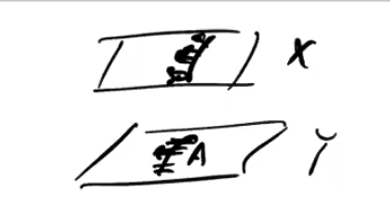
\includegraphics[width=3.64583in,height=\textheight]{figures/image_2020-11-15-01-41-25.png}
\caption{Image}
\end{figure}

\end{remark}

\begin{remark}

There are some equivalent definitions of a morphism being étale:

\begin{itemize}
\item
  Smooth of relative dimension zero
\item
  Locally finite presentation and \emph{formally étale}
\item
  Locally \emph{standard étale}, i.e.~for each \(x\in X\) with
  \(y\coloneqq f(x)\), there exists a \(U\ni x, V\ni y\) such that
  \(f(U) \subseteq V\) and
  \(V=\operatorname{Spec}(R), U = \operatorname{Spec}\qty{R[x]_h / g}\)
  (where we localize at \(h\)) such that the derivative \(g'\) is a unit
  in \(R[x]_h\) and \(g\) is monic.
\end{itemize}

For this last definition, thinking of \(\operatorname{Spec}(R[x])\) as
\(R\times {\mathbb{A}}^n\), what happens when modding out by a
polynomial \(g\)? This yields a curve cutting out the roots of \(g\).
Inverting \(h\) deletes the locus where \(h\) vanishes, and \(g'\) being
a unit means that the \(g\) has no double roots in the fibers. In other
word, the deleted locus passes through all double roots:

\begin{figure}
\centering
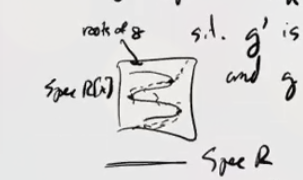
\includegraphics[width=3.64583in,height=\textheight]{figures/image_2020-11-15-01-47-05.png}
\caption{Image}
\end{figure}

\end{remark}

\begin{exercise}[?]

Check that standard étale morphisms are étale, and try to understand the
proof that all étale morphisms are locally standard étale.

\end{exercise}

\begin{example}[Example of an étale morphism]

\envlist

\begin{itemize}
\item
  Multiplication by \([n]\) on an elliptic curve if
  \(n \in {\mathbb{Z}}\) is invertiable in the base field.
\item
  Take \({\mathbb{G}}_m = \operatorname{Spec}k[t, t^{-1}]\), and the map
  \begin{align*}  
  {\mathbb{G}}_m &\to {\mathbb{G}}_m \\
   t^m &\mapsfrom t
  ,\end{align*}
  where \(n\) is prime to \(\operatorname{ch}(k)\).\footnote{Here we use
    the convention that everything is prime to zero. Also note that this
    map is in fact finite étale.}
\end{itemize}

\end{example}

\begin{exercise}[?]

Show that the last map above is étale.

\emph{(Hint: use the fact that
\({\frac{\partial }{\partial t}\,} (t^n) = nt^{n-1}\), which is a
unit.)}

\end{exercise}

\begin{example}[?]

Consider the map
\begin{align*}  
{\mathbb{G}}_m &\hookrightarrow{\mathbb{A}}^1 \\
k[t, t^{-1}] &\mapsfrom k[t]
.\end{align*}
We need to check 3 things:

\begin{itemize}
\tightlist
\item
  Locally finite presentation,

  \begin{itemize}
  \tightlist
  \item
    This is a finitely presented ring map, since you just need to adjoin
    an inverse of \(t\), one element and one relation.
  \end{itemize}
\item
  Flat,

  \begin{itemize}
  \tightlist
  \item
    Since open embeddings are flat,
  \end{itemize}
\item
  \(\Omega^1_{{\mathbb{G}}_m / {\mathbb{A}}^1} = 0\),

  \begin{itemize}
  \tightlist
  \item
    True for a Zariski open embedding.
  \end{itemize}
\end{itemize}

Note that this is finite onto its image.

\end{example}

\begin{proposition}[?]

Any open immersion is étale.

\end{proposition}

Note that we actually already checked this!

\begin{example}[An étale morphism that is not finite onto its image]

Use the fact that \({\mathbb{G}}_m\) is
\({\mathbb{A}}^1\setminus\left\{{\mathbf{0}}\right\}\), so take
\({\mathbb{G}}_m \setminus\left\{{1}\right\}\) and the map
\begin{align*}  
{\mathbb{G}}_m\setminus\left\{{1}\right\} &\to {\mathbb{G}}_m \\
t^2 &\mapsfrom t
.\end{align*}

What's the picture? For the squaring map, there are two square roots:

\begin{figure}
\centering
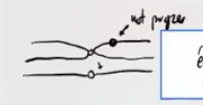
\includegraphics{figures/image_2020-11-15-02-01-04.png}
\caption{Image}
\end{figure}

This is an étale surjection but not finite étale, since it is not
proper. This also gives a counterexample to étale morphisms always
looking like covering spaces, since here that may be true locally but
doesn't hold globally.

\end{example}

\begin{warnings}

This is an important example to keep in mind, because you'll often see
arguments that treat étale maps as though they were finite onto their
image.

\end{warnings}

\begin{example}[?]

Take a finite separable field extension, taking \(\operatorname{Spec}\)
of it yields an étale map.

\end{example}

Now for some non-examples:

\begin{example}[A finite map which is not etale]

Take \(X = \operatorname{Spec}k[x, y] / xy\), which looks like the
following:

\begin{figure}
\centering
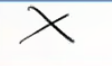
\includegraphics[width=3.64583in,height=\textheight]{figures/image_2020-11-15-02-04-46.png}
\caption{\(X\)}
\end{figure}

Then the normalization \(\tilde X\to X\) is not étale, since it is not
flat.

\end{example}

\begin{example}[A finite flat map which is not etale]

Take the map
\begin{align*}  
{\mathbb{A}}^1 &\to {\mathbb{A}}^1 \\
t^2 &\mapsfrom t
.\end{align*}

The picture is the following:

\begin{figure}
\centering
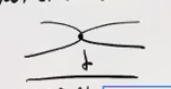
\includegraphics{figures/image_2020-11-15-02-07-04.png}
\caption{Image}
\end{figure}

This is note étale since it is ramified at zero. We can compute
\begin{align*}  
\Omega_f^1 = k[t]\, dt / d(t^2) = k[t] dt/ 2t\, dt
,\end{align*}
where \(2t\,dt\) does not generate this module. This is supported at
\(t=0\) if \(\operatorname{ch}\neq 2\).

\end{example}

\begin{example}[?]

A finite flat morphism such that \(\Omega_{X/Y}^1\) is not torsion: a
hint is that the previous example almost works, with a slight
modification. Let \(\operatorname{ch}k = p\), and take
\begin{align*}  
{\mathbb{A}}^1 &\xrightarrow{F} {\mathbb{A}}^1 \\
t^p &\mapsfrom t
.\end{align*}
Then \(\Omega_f^1 = k[t]\, dt / d(t^p) = k[t]\,dt\) since \(d(t^p) = 0\)
in characteristic \(p\). This yields line bundles (?), so it is not
torsion.

\end{example}

\begin{remark}

This map has a name: \textbf{the relative Frobenius}. In general,
looking at Frobenii, the Kahler differentials will be very big. You
might not be used to this: in characteristic zero, a map of relative
dimension zero is generically étale. In this case, the Kahler
differentials will always be torsion.

\end{remark}

\begin{example}[?]

Consider a map
\begin{align*}  
{\mathbb{A}}^m &\xrightarrow{f_1, \cdots, f_m} {\mathbb{A}}^m
,\end{align*}
since such a map is given by a system of \(m\) polynomials in \(m\)
variables. Then \(f\) is étale is a neighborhood of \(\mathbf{a}\) if
\(\det \qty{{\frac{\partial f_i}{\partial x_j}\,} \Big|_{\mathbf{a}} }\)
is a unit.

\end{example}

\hypertarget{properties-of-uxe9tale-morphisms}{%
\subsubsection{Properties of Étale
Morphisms}\label{properties-of-uxe9tale-morphisms}}

\begin{proposition}[Some properties of étale morphisms]

\envlist

\begin{enumerate}
\def\labelenumi{\arabic{enumi}.}
\tightlist
\item
  Open immersions are étale
\item
  Compositions of étale morphisms are étale\footnote{What do you have to
    check? Locally finite presentation, flat, and unramified are all
    preserved. The one that may be tricky is remaining unramified, a
    hint is to use the cotangent exact sequence for \(\Omega^1_{X/Y}\).}
\item
  Base change of étale morphisms are étale, i.e.~
\end{enumerate}

\begin{enumerate}
\def\labelenumi{\arabic{enumi}.}
\setcounter{enumi}{3}
\tightlist
\item
  There is a 2 out of 3 property: If \(\phi \circ \psi\) and \(\phi\)
  are étale, then \(\psi\) is étale.
\end{enumerate}

\end{proposition}

\begin{exercise}[?]

Show property 4 above.

\end{exercise}

\begin{proposition}[?]

Étale morphisms on varieties over an algebraically closed field induce
isomorphisms on complete local rings at closed points.

\end{proposition}

\begin{exercise}[?]

Prove this! Hint: use the criterion for formal étaleness. There's an
evident map one way on local rings coming from your étale morphism, and
you need to produce the inverse map.

\end{exercise}

\begin{exercise}[?]

\(\danger\) If \(\psi\) is étale and \(\phi\circ\psi\) is étale, it is
not necessarily the case that \(\phi\) is étale. Come up with an
example!

\end{exercise}

\begin{corollary}[An informal statement]

Any property that can be checked at the level of complete local rings is
true for the source of an étale morphism if it is true for the target.

\end{corollary}

Why? If you want to check a property for complete local rings on the
source, note that the map induces an isomorphism of complete local
rings.

\hypertarget{generalizing-topologies}{%
\subsection{Generalizing Topologies}\label{generalizing-topologies}}

\hypertarget{sites}{%
\subsubsection{Sites}\label{sites}}

The notion of a \emph{site} will be a generalization of topological
spaces and sheaves. The idea is we'll generalize sheaf cohomology to
this setting. On a nice space like a manifold, singular cohomology is
isomorphic to the sheaf cohomology of the constant sheaf
\(\underline{{\mathbb{Z}}}\). Here we'll find some version of a sheaf
where étale cohomology with \({\mathbb{Z}}/\ell^n{\mathbb{Z}}\)
coefficients will be the sheaf cohomology with the constant sheaf
\(\underline{{\mathbb{Z}}/\ell^n{\mathbb{Z}}}\).

\begin{question}

What parts of the definition of a topological space are needed to define
the notion of a sheaf?

\end{question}

\begin{remark}

Recall that the \emph{sheaf condition} is given in two parts:

\begin{enumerate}
\def\labelenumi{\arabic{enumi}.}
\item
  A section is determined by its value on a cover, and
\item
  Sections can be glued when they agree on intersections.
\end{enumerate}

\end{remark}

\begin{answer}

\envlist

\begin{enumerate}
\def\labelenumi{\arabic{enumi}.}
\tightlist
\item
  As in presheaves, a notion of open sets and inclusions. (I.e., a
  category of open sets.)\footnote{Recall that a presheaf on \(X\) is a
    contravariant functor out of the category of open sets of \(X\).}\footnote{The
    notion of a presheaf on \(X\) doesn't know much about the actual
    topology of \(X\). If two spaces have the coarsest topology, so the
    only opens are \(X, \emptyset\), then the categories of open sets
    are equivalent, and every presheaf on them will be the same.}
\end{enumerate}

We'd also like to make sense of the sheaf condition:

\begin{enumerate}
\def\labelenumi{\arabic{enumi}.}
\setcounter{enumi}{1}
\item
  Collections of morphisms which are ``covers'', remembering which
  collections of opens cover a space, and
\item
  The existence of certain fiber products (intersections).
\end{enumerate}

\end{answer}

\begin{remark}

The motivation for (3) above is that for \(U, V \subseteq X\), we can
form \(U\times V = U\cap V\).

\end{remark}

We will make the following preliminary definition:

\begin{definition}[Sites/Grothendieck Topologies]\label{def:site}

A category \(\mathcal{C}\) with a collection of \emph{covering
families}\footnote{How to think of this: elements in this collection
  cover \(X\).}
\begin{align*}
\left\{{X_\alpha \xrightarrow{f_\alpha} X {~\mathrel{\Big|}~}\alpha\in A}\right\}
\end{align*}
such that several axioms are satisfied.

\end{definition}

We'll discuss the axioms next time, they just capture the notion of what
a cover of a topological space should look like.

\begin{warnings}

There are at least three different notions of this definition! The one
above is perhaps the least general but the easiest to work with.

\end{warnings}

\begin{example}[?]

For \(X\) a topological space, \(\mathcal{C}\) the category of open sets
in \(X\), then \(\left\{{U_\alpha\to U}\right\}\) is a covering family
if the \(U_\alpha\) cover \(U\), i.e.~\(U = \cup_\alpha U_\alpha\).

\end{example}

\begin{example}[More exotic]

Let \(M\) be a manifold and \(\mathcal{C}\) be the category of manifolds
over \(M\), so all \(M' \xrightarrow{f} M\) such that \(f\) is locally
an isomorphism. Note that these are smooth local homeomorphisms. Let
\begin{align*}
\left\{{M_\alpha \xrightarrow{f_\alpha} M}\right\} \text{ if } \bigcup_\alpha \operatorname{im}(f_\alpha) = M
\end{align*}

\end{example}

\begin{example}[Another exotic example]

Let \(X\) be a scheme and consider \(X_{\text{et}}\) the category of all
étale \(Y/X\): so the objects are schemes \(Y\) admitting an étale
morphism \(Y\to X\). Then \(\left\{{X_\alpha\to X}\right\}\) is a
covering family if \(\cup\operatorname{im}(f_\alpha) = X\).

\end{example}

This will be the fundamental object, and we'll define étale cohomology
by defining sheaves on this category, taking a constant sheaf
\(\underline{{\mathbb{Z}}/\ell^n{\mathbb{Z}}}\), and we'll take sheaf
cohomology.

\hypertarget{lecture-3}{%
\section{Lecture 3}\label{lecture-3}}

\hypertarget{defining-sites}{%
\subsection{Defining Sites}\label{defining-sites}}

Today: we'll discuss sites, which generalizes the category of open sets
over a topological space. The goal is to generalize spaces and sheaves
to categories, and to define a sheaf we need

\begin{enumerate}
\def\labelenumi{\arabic{enumi}.}
\item
  A notion of a \emph{cover}, and
\item
  A notion of intersections/fiber products of open sets.
\end{enumerate}

\begin{definition}[Grothendieck Topology / Sites]

A \textbf{Grothendieck topology} on \(\mathcal{C}\) or a \textbf{site}
on \(\mathcal{C}\) is the data of for each
\(X\in \mathrm{Ob}(\mathcal{C})\) a collection of sets of morphism
\(\left\{{X_\alpha \to X}\right\}\) (\emph{covering families})
satisfying

\begin{itemize}
\item
  Intersections exist: If \(X_\alpha\to X\) appears in a covering family
  and \(Y\to X\) is arbitrary, the fiber product \(X_\alpha\times_X Y\)
  exists.
\item
  Intersecting with a cover again yields a cover: If
  \(\left\{{X_\alpha\to X}\right\}\) is a covering family and \(Y\to X\)
  is arbitrary, then the covering family can be pulled back:
  \(\left\{{Y\times_X X_\alpha\to Y}\right\}\) is again a covering
  family.\footnote{When \(\mathcal{C}\) was the category of open sets of
    a space \(X\), the existence of this morphism \(Y\to X\) says
    \(Y \subseteq X\) is an open subset, and thus intersecting \(Y\)
    with any open cover of \(X\) yields an open cover of \(Y\).}
\item
  Compositions of coverings are again coverings: If
  \(\left\{{X_\alpha\to X}\right\}_{\alpha}\) and
  \(\left\{{X_{\alpha\beta} \to X_\alpha}\right\}_{\alpha,\beta}\) are
  covering families, then you can compose, i.e.~taking the set of all
  possible ways of composing
  \(\left\{{X_{\alpha\beta} \to X_\alpha \to X}\right\}\) is again a
  covering family.\footnote{For spaces, this says if you have a cover of
    an open set by subsets and a cover of each of those subsets, the
    entire set has been covered.}
\item
  Isomorphisms are covers: If \(X\xrightarrow{\sim_f} Y\) is an
  isomorphism, then the singleton family
  \(\left\{{X\xrightarrow{f} Y}\right\}\) is a covering family.
\end{itemize}

\end{definition}

\hypertarget{examples-of-sites}{%
\subsubsection{Examples of Sites}\label{examples-of-sites}}

\begin{example}[The motivating example]

If \(X\) is a topological space, define \(\mathcal{C}\) whose objects
are open subsets of \(X\) where there is a unique morphism \(U\to V\)
iff \(U\subseteq V\). Then \(\left\{{U_\alpha \to U}\right\}\) is a
covering family if \(\bigcup_\alpha U_\alpha = U\).

\end{example}

\begin{example}[The small étale site]

Let \(X\) be a scheme, and define the small étale site
\(X_{\text{ét}}\): the category whose objects are étale morphisms
\(Y\xrightarrow{f} X\) where morphisms are maps over \(X\):

Note that \(g\) is étale by the 2 out of 3 property.

Then \(\left\{{X_\alpha\to X}\right\}\) is a covering family if the set
theoretic images satisfy
\(\bigcup_\alpha \operatorname{im}(f_\alpha) = X\).

\end{example}

\begin{example}[The big étale site]

Again let \(X\) be a scheme, and define \(X_{\mathrm{Et}}\) the category
whose objects are all \(X{\hbox{-}}\)schemes (where we no longer require
the maps to be étale). In other words, this is the overcategory of
\(X\): the category of schemes over \(X\). Then
\(\left\{{U_\alpha\xrightarrow{f_\alpha}U}\right\}\) is a covering
family if all of the \(f_\alpha\) are étale and
\(\bigcup_\alpha \operatorname{im}(f_\alpha) = U\).

\end{example}

Note the difference: in the small site, we included only étale
\(X{\hbox{-}}\)schemes, vs all \(X{\hbox{-}}\)schemes in the big site.
In both cases, the notion of covering families are the same.

\begin{example}[?]

Let \(X\) be a complex analytic space (e.g.~a complex manifold), then
there is an analytic étale site whose objects are complex analytic
spaces \(Y\xrightarrow{f} X\) such that locally on \(Y\), \(f\) is an
analytic isomorphism. Note that this includes covering spaces. The
morphisms will be morphisms over \(X\) creating commuting triangles, and
the covers are the usual covers.

\end{example}

\begin{remark}

This category is part of what motivates the definition of the étale
topology. This is what we're trying to imitate. E.g. if you have a
complex algebraic variety, taking its analytification will be one of
these. This site will show up later when we compare étale cohomology to
singular cohomology.

\end{remark}

\begin{remark}

We haven't said what it means to be a sheaf yet, but Grothendieck
topologies behave in somewhat unexpected ways. The category of sheaves
of the analytic étale cohomology,
\({\operatorname{Sh}}(X_{\mathrm{an{\hbox{-}}et}})\), is canonically
equivalent to \({\operatorname{Sh}}(X^{\mathrm{top}})\). Thus sometimes
the category of sheaves over a site doesn't remember the site, i.e.~two
different sites can have the same category of sheaves. On the RHS we had
a category of open subsets, whereas on the LHS we included things like
covering spaces. We'll see later that there is a notion of morphisms of
sites, and there is a morphism inducing this equivalence.

Proving this isomorphism will be an exercise, here's an outline of why
it's true: suppose you have a cover of \(X\) in this category, i.e.~a
family of local analytic isomorphisms. Given any of these, you can cover
by subsets for which these are isomorphisms onto their images.

\end{remark}

\begin{definition}[fppf]

The letter \textbf{fppf} stand for \textbf{faithfully flat and finite
presentation}. \footnote{The letters don't precisely match up here
  because this comes from a French acronym.}

\end{definition}

\begin{example}[The fppf topology]

There are small and big sites here: we define
\(X_{\mathrm{\operatorname{fppf}}}\) whose objects are fppf morphism
\(Y\to X\), with morphisms as triangular diagrams of morphisms over
\(X\), and covers are the usual covers. Note that replacing fppf
morphisms with flat morphisms would yield an equivalent definition here.

\end{example}

\begin{example}[?]

If \(X\) is a scheme, then the small Zariski topology is
\(X_{\mathrm{zar}}\) whose objects are
\({\operatorname{Op}}(X^{\mathrm{top}})\), the Grothendieck topology of
the corresponding topological space, and we take the usual notion of
covers. There is a big Zariski topology \(X_{\mathrm{Zar}}\) whose
category is all \(X{\hbox{-}}\)schemes
\(\left\{{U_\alpha\xrightarrow{f_\alpha} U}\right\}\) with \(f_\alpha\)
open embeddings and \(\bigcup_\alpha \operatorname{im}(f_\alpha) = U\).

\end{example}

\begin{example}[?]

Some other examples:

\begin{itemize}
\item
  The \textbf{Nisnevich} topology, which lives between the Zariski and
  the étale topology,
\item
  The \textbf{crystalline} site, used to define crystalline cohomology,
\item
  The \textbf{infinitesimal} site,
\item
  The \textbf{cdh} topology, the \textbf{arc} topology, the \textbf{rh}
  topology, and many more.
\end{itemize}

\end{example}

\hypertarget{toward-sheaves-of-sites}{%
\subsection{Toward Sheaves of Sites}\label{toward-sheaves-of-sites}}

\begin{definition}[Presheaf]

For \(\mathcal{D}\) a category, a \(\mathcal{D}{\hbox{-}}\)valued
\textbf{presheaf} is a contravariant function
\(F:\mathcal{C}\to \mathcal{D}\).

\end{definition}

\begin{remark}

This makes no reference to any Grothendieck topology.

\end{remark}

\begin{example}[?]

If \(X\) is a topological space, a \(\mathcal{D}{\hbox{-}}\)valued
presheaf of \(X\) is equivalent to a presheaf on
\({\operatorname{Op}}(X)\).

\end{example}

We can now define a sheaf. What's the motivation? For \(X\) a
topological space, it's a sheaf satisfying some conditions: its sections
are determined by an open cover, and given sections agreeing on overlaps
allows gluing. This can be captured by a specific diagram, which is what
we will use here.

Recall the definition of a \textbf{site} (\cref{def:site}): in short, a
category equipped with the Grothendieck topology.

\begin{definition}[Sheaf]

A \textbf{sheaf} \(F\) is presheaf such that

is an \emph{equalizer} diagram for all covering families
\(\left\{{U_\alpha \to U}\right\}\).

\end{definition}

\begin{remark}

The diagram arises due to the fact that if we have a bunch of maps
coming from a cover, since we have a contravariant functor, we get a map
into the product. We then look at the intersections of all
\(U_{\alpha}, U_{\alpha'}\).

The two arrows occurring come from the projections:

where we use the fact that since \(F\) is a contravariant functor, it
induces maps going the other way.

What does being an equalizer mean, say if \(F\) is set-valued?
``Exactness'' at the middle term is the gluing condition, and exactness
at the first term is injectivity, i.e.~a section (the values of \(F\) on
\(U\)) are determined by its values on a cover (by \(F(U_\alpha)\)).
Note that in fact \(F(U)\) is the limit of this diagram. The gluing
condition is more precisely that if we're given
\((s_\alpha) \in \prod_\alpha F(U_\alpha)\) such that
\(F(\pi_1)(s_\alpha) = F(\pi_2)(s_\alpha)\), then \((s_\alpha)\) comes
from \(F(U)\).

\end{remark}

\begin{definition}[Morphisms of sheaves and presheaves]

A \textbf{morphism} \(F_1\to F_2\) of either presheaves or sheaves is a
natural transformation of functors.

\end{definition}

\hypertarget{examples-of-sheaves-of-sites}{%
\subsubsection{Examples of Sheaves of
Sites}\label{examples-of-sheaves-of-sites}}

\begin{theorem}[?]

Any representable functor is a sheaf on the étale site
\(X_{\text{Ét}}\). In fact, any such functor is a sheaf on the big fppf
site \(X_{\mathrm{\operatorname{Fppf}}}\): the category of all
\(X{\hbox{-}}\)schemes with covers as fppf covers, which are maps that
are flat and jointly surjective.

\end{theorem}

\begin{example}[Examples of sheaves on the étale site]

Take \(\mu_n\) the functor represented by
\(\mu_n \coloneqq\operatorname{Spec}k[t] / t^{n-1}\). For \(U\) an
\(X{\hbox{-}}\)scheme, we can evaluate in the following way:
\begin{align*}  
\mu_n(U) = \left\{{f\in {\mathcal{O}}_U(U) {~\mathrel{\Big|}~}f^n = 1}\right\}
.\end{align*}

\end{example}

\begin{example}[?]

We define a sheaf of the étale site as
\({\mathcal{O}}^{\text{ét}}_X(U) = {\mathcal{O}}_U(U)\) where we've said
what the values are. This is a sheaf that is represented by
\({\mathbb{A}}^1_{/X}\).

\end{example}

\begin{example}[?]

The constant sheaf \(\underline{\mathbb{Z}/\ell^n\mathbb{Z}}\). How can
we prove it is a sheaf, given the theorem, and determine what its values
are? This is represented by
\(\qty{\mathbb{Z}/\ell^n\mathbb{Z}} \times X\), i.e.~taking the disjoint
union of \(\ell^n\) copies of \(X\). The values are given by
\begin{align*}  
\underline{\mathbb{Z}/\ell^n\mathbb{Z}}(U) =  \hom_{{\operatorname{Top}}}(U^{{\operatorname{Top}}}, \mathbb{Z}/\ell^n\mathbb{Z})
,\end{align*}
where we give the set \(\mathbb{Z}/\ell^n\mathbb{Z}\) the discrete
topology and take morphisms to be continuous maps.

\end{example}

\begin{warnings}

The constant sheaf \(\underline{S}\) doesn't associate \(S\) to every
open set: it instead associates \(S^d\) where \(d\) is the number of
components. The former would only be a presheaf, and not a sheaf.

\end{warnings}

\begin{example}[?]

We can take the sheaf
\({\mathbb{G}}_m(U) \coloneqq{\mathcal{O}}_U(U)^{\times}\), whose values
are obtained by taking the global sections of the structure sheaf and
only keeping the units. This is represented by
\begin{align*}
{\mathbb{G}}_{m, X} = \operatorname{Spec}{\mathbb{Z}}[t, t^{-1}] \underset{\scriptscriptstyle {\operatorname{Spec}{\mathbb{Z}}} }{\times} X
\end{align*}
Why does this represent this functor? Mapping into this requires that
\(t\) goes to an invertible function, which yields the isomorphism.

\end{example}

\begin{remark}

Note that all of these functors take values in abelian groups, which is
a consequence of the fact that the representing objects are group
schemes. In fact, one definition of a group scheme is that the functor
it represents factors through groups.

\end{remark}

\begin{example}[?]

Take the functor \({\mathbb{P}}^n(U) \coloneqq\hom(U, {\mathbb{P}}^n)\).
This functor can be written down as a line bundle on \(U\) with a
surjective map from \({\mathcal{O}}_U \to {\mathcal{O}}_U^n\) (?), the
functor represented by projective space, and that's also a sheaf that is
necessarily representable but not an abelian one.

\end{example}

Some things we still need to get to:

\begin{itemize}
\tightlist
\item
  A proof that \(\underline{\mathbb{Z}/\ell^n\mathbb{Z}}\) is actually a
  sheaf,
\item
  A proof that the category of sheaves on the big étale site
  \(X_\text{Ét}\)\footnote{Note that a sheaf on the big étale site
    necessarily restricts to a sheaf on the small étale site, since
    covers in the small site are also covers in the big site.} with
  values in \(\mathbf{Ab}\) is abelian and has enough injectives.
\end{itemize}

\hypertarget{uxe9tale-cohomology-a-preliminary-definition}{%
\subsection{Étale Cohomology: A Preliminary
Definition}\label{uxe9tale-cohomology-a-preliminary-definition}}

\begin{definition}[Imprecise: étale cohomology]

Let \(\mathcal{F}\) be a sheaf and define a functor
\(\Gamma_X: \mathcal{F}\to \mathcal{F}(X)\) sending it to its values on
\(X\). Then the \textbf{étale cohomology} of \(X\) is defined by
\begin{align*}  
H^i(X_\text{ét}, \underline{\mathbb{Z}/\ell^n\mathbb{Z}}) \coloneqq R^i \Gamma_X(\underline{\mathbb{Z}/\ell^n\mathbb{Z}})
,\end{align*}
the right-derived functors of \(\Gamma_X\).

\end{definition}

\begin{remark}

This definition is incomplete, and in particular, it's highly
non-obvious that this category of abelian sheaves is abelian. E.g.
usually when proving that the category of abelian sheaves on a
topological space has cokernels, you use sheafification: you take the
cokernel of a map of presheaves, which is a presheaf, and sheafify it.
Here, we don't know how to sheafify a presheaf on a site. The usual
construction involves forming the \emph{espace étalé} and taking
sections does not work for a site, you need a genuinely different
argument.

\end{remark}

\begin{warnings}

Even showing cokernels exist in the category of abelian sheaves on a
site is nontrivial. Try as an exercise!

\end{warnings}

\begin{remark}

What will be true in general is that this category will be an \(AB5\)
abelian category, and having enough injectives is all that's
additionally needed. This comes from machinery developed in
Grothendieck's Tohoku paper, and we'll sketch part of the proof.

\end{remark}

Properties of these sheaves are not so obvious, and depend on the site
you're working over:

\begin{example}[?]

Consider the map
\begin{align*}  
{\mathbb{G}}_m &\to {\mathbb{G}}_m \\
t^m &\mapsfrom t
,\end{align*}
where \(n\) is invertible over the base, e.g.~if we're over a field of
characteristic coprime to \(n\). This yields a map of sheaves in two
different settings. In \(X_{\mathrm{Zar}}\) we have
\begin{align*}  
{\mathcal{O}}^{\times}&\to {\mathcal{O}}^{\times}\\
f &\mapsto f^n
.\end{align*}

We can look at this in \(X_{\text{ét}}\), yielding
\begin{align*}  
{\mathcal{O}}_\text{ét}^{\times}&\to {\mathcal{O}}_\text{ét}^{\times}\\
f &\mapsto f^m
.\end{align*}

\begin{claim}

This map is not an epimorphism on \(X_{\mathrm{Zar}}\) but is on
\(X_{\text{ét}}\)

\end{claim}

\begin{proof}[?]

It suffices to give one example: take
\(X = \operatorname{Spec}{\mathbb{R}}\) and \(n=2\), and since this is
just a point, the sheaf is determined by its values. So is the map
\begin{align*}  
{\mathbb{R}}^{\times}&\to {\mathbb{R}}^{\times}\\
t &\mapsto t^2
\end{align*}
surjective? The answer is no, of course, since its image is
\({\mathbb{R}}_{\geq 0}\).

This will be surjective on \(X_{\text{ét}}\) if \(n\) is invertible on
\(X\). If we were in usual topological spaces, we would want to show
that given any section of the sheaf on an open set, it can be refined.
Here we want to pass to an étale cover so that section has an \(n\)th
root. So given \(f\in {\mathbb{G}}_m(U)\), we want an étale cover of
\(U\) so that \(f\) obtains an \(n\)th root. An invertible function is a
map \(U\to {\mathbb{G}}_m\), and we can form the square

The RHS map is étale since \(n\) is invertible, and the fiber product is
étale since étale morphisms are preserved by base change.

\begin{claim}

\(f\) has an \(n\)th root upstairs. (Verify!)

\end{claim}

There's a more concrete way of writing this: note that
\({\mathbb{A}}^1_{U, z} = \operatorname{Spec}k[t]\), so take the
subscheme cut out by \(V(z^n - f)\). This will be an étale cover of
\(U\) (the same one in fact) and \(z\) is now an \(n\)th root.

\end{proof}

\end{example}

\begin{exercise}[?]

Check the details! Namely that this argument implies that this map of
sheaves is an epimorphism.

\end{exercise}

\begin{remark}

This map of sheaves
\({\mathbb{G}}_m \xrightarrow{z^m \mapsfrom z} {\mathbb{G}}_m\), noting
that if \(n\) is not invertible this will not be an epimorphism, will
always be an epimorphism in
\({\operatorname{Sh}}(X_\mathrm{\operatorname{fppf}})\) since this map
is flat and finitely presented.

\end{remark}

\hypertarget{preview-morphisms-of-sites}{%
\subsection{Preview: Morphisms of
Sites}\label{preview-morphisms-of-sites}}

\begin{definition}[Morphisms of Sites]

Suppose \(T_1, T_2\) are sites (categories with covering families), then
a \textbf{continuous map of sites} \(f:T_1 \to T_2\) is a functor
\(T_2 \to T_1\)\footnote{Note that this functor goes in the opposite
  direction of the original map.} that preserves fiber products and
sends covering families to covering families.

\end{definition}

\begin{example}[?]

A continuous map
\(f\in {\operatorname{Hom}}_{\operatorname{Top}}(X, Y)\) induces a map
\begin{align*}  
{\operatorname{Op}}(Y) &\to {\operatorname{Op}}(X) \\
U &\mapsto f^{-1}(U)
.\end{align*}

\end{example}

\begin{exercise}[?]

Check that this is a continuous map of sites.

\end{exercise}

Next time: a bunch of examples.

\hypertarget{lecture-4-descent}{%
\section{Lecture 4: Descent}\label{lecture-4-descent}}

Last time: sites, sheaves, and morphisms of sites. Today: descent, which
is how we'll see that many familiar objects are sheaves on the étale
site, such as representable functors or quasicoherent sheaves.

\hypertarget{reminder}{%
\subsection{Reminder}\label{reminder}}

\begin{definition}[A continuous map of sites]

Given two sites \((C, T_1)\) and \((D, T_2)\) where \(C, D\) are
categories and the \(T_i\) are collections of covering families, a
\textbf{morphism} is a functor \(f^{-1} :D\to C\) such that

\begin{enumerate}
\def\labelenumi{\arabic{enumi}.}
\tightlist
\item
  \(f^{-1}\) preserves fiber products.
\item
  \(f^{-1}\) sends covering families to covering families.
\end{enumerate}

\end{definition}

\begin{example}[?]

The main example: for \(f:X\to Y\) a map of topological spaces, the
functor \(F: {\operatorname{Op}}(Y) \to {\operatorname{Op}}(X)\) given
by \(F(U) \coloneqq f^{-1}(U)\) sending an open set to its preimage.

\end{example}

\begin{exercise}[Check!]

Check that this is a continuous map of sites.

\end{exercise}

\begin{example}[?]

Suppose \(X\) is a scheme, then there is a natural map of sites from
\(X_{\mathrm{\operatorname{Fppf}}}\) (all \(X{\hbox{-}}\)schemes where
covers are collections of jointly surjective flat morphism) to
\(X_{\text{Ét}}\) (all \(X{\hbox{-}}\)schemes where covers are jointly
surjective étale morphisms) to \(X_{\text{ét}}\) (étale
\(X{\hbox{-}}\)schemes with morphisms over \(X\)) to
\(X_{{\mathrm{zar}}}\) (the open subsets of \(X\) with morphisms given
by inclusions and covers the usual covers). The maps here are inclusions
going the other way.

\end{example}

\begin{exercise}[Check!]

Check that these are continuous maps of sites.

\end{exercise}

\begin{remark}

\envlist

On terminology:

\begin{itemize}
\item
  What we've been calling a site or a Grothendieck topology is sometimes
  called a \emph{Grothendieck pretopology}. The major difference is that
  you don't have to assume the existence of fiber products.
\item
  You may also see the notion of a \textbf{topos}, which is the category
  of sheaves on a site.
\end{itemize}

\end{remark}

\hypertarget{setting-up-descent}{%
\subsection{Setting up Descent}\label{setting-up-descent}}

\begin{question}

\envlist

\begin{enumerate}
\def\labelenumi{\arabic{enumi}.}
\item
  We've said what it means to be a sheaf on a site, how do we check that
  a given functor is a sheaf on \(X_{\text{ét}}\) or
  \(X_{\mathrm{\operatorname{fppf}}}\)?
\item
  How do we construct such sheaves?
\end{enumerate}

\end{question}

\begin{theorem}[Ways of constructing sheaves]

\envlist

\begin{enumerate}
\def\labelenumi{\arabic{enumi}.}
\item
  If \(Y\) is an \(X{\hbox{-}}\)scheme (i.e.~a scheme equipped with a
  map to \(X\)) then the functor \(Z \to \hom_X(Z, Y)\) is a sheaf on
  \(X_{\mathrm{\operatorname{Fppf}}}, X_{\text{Ét}}, X_{\text{ét}}\),
  etc.
\item
  Suppose \(\mathcal{F}\) is a quasicoherent sheaf on \(X\), so
  \(\mathcal{F}\in {\mathrm{QCoh}}(X)\), the functor of taking global
  sections:
\end{enumerate}

is a sheaf on
\(X_{\mathrm{\operatorname{Fppf}}}, X_{\text{Ét}}, X_{\text{ét}}\), etc.

\end{theorem}

\begin{definition}[$\mathcal{F}^\text{étale}$]

The sheaf associated to the above functor on \(X_{\text{ét}}\) will be
denoted \(\mathcal{F}^\text{étale}\).

\end{definition}

\begin{proof}[of 2]

Suppose we have an fppf cover of \(X\)

\end{proof}

\begin{question}

Suppose \(\mathfrak{F}\in {\mathrm{QCoh}}(X)\). When does it come from a
quasicoherent sheaf on \(X\)? I.e., when is there a quasicoherent sheaf
\(\mathcal{F}'\) on \(X\) and an isomorphism between its pullback to
\(U\) and \(\mathcal{F}\)? What extra structure do you need to
``descend'' to \({\mathrm{QCoh}}(X)\), i.e.~to pick such an isomorphism?

\end{question}

\begin{question}

Given \(\mathcal{F}_1, \mathcal{F}_2 \in {\mathrm{QCoh}}(U)\) and a
morphism
\(f: { \left.{{\mathcal{F}_1}} \right|_{{U}} } \to { \left.{{\mathcal{F}_2}} \right|_{{U}} }\),
when does \(f\) come from \(X\)?

\end{question}

\begin{remark}

If \(X = \operatorname{Spec}k\) and \(U\) is a finite separable
extension, then this question is exactly what Galois descent is about!

\end{remark}

\begin{example}[(a motivating one)]

\(U = {\coprod}U_i \to X\) is a Zariski cover. If we have a sheaf on
\(U\), what extra data do we need to get a sheaf on \(X\)? We need
isomorphisms
\({ \left.{{\mathcal{F}_i }} \right|_{{U_i\cap U_j}} } \xrightarrow{\sim} { \left.{{\mathcal{F}_j}} \right|_{{U_i\cap U_j}} }\)
(gluing data) where each \(\mathfrak{F}_i\) is the sheaf given on
\(U_i\). We also need a cocycle condition on triple intersections. Given
this data, gluing yields a sheaf on \(X\). This may be familiar from
vector bundles. Thus to give a sheaf, it suffices to specify gluing
data.

Morphisms \(\mathcal{F}\to \mathcal{G}\) is the same as morphisms
\({ \left.{{\mathcal{F}}} \right|_{{U_i}} } \to { \left.{{\mathcal{G}}} \right|_{{U_i}} }\)
which commute with the gluing data. We'd like to generalize this notion
of commuting with gluing data to more general types of covers.

\end{example}

\begin{definition}[Descent data for quasicoherent sheaves]

Suppose \(U\xrightarrow{f}X\) is a morphisms, then \textbf{descent data}
for a quasicoherent sheaf on \(U/X\) is the following:

\begin{enumerate}
\def\labelenumi{\arabic{enumi}.}
\tightlist
\item
  A sheaf \(\mathcal{F}\in {\mathrm{QCoh}}(U)\).
\item
  Gluing data: If we take the fiber product of \(U\) with itself,
  mapping to \(U\) under 2 different projections\footnote{If \(U\) was
    an open cover, this would correspond to intersections of elements in
    the cover.},
\end{enumerate}

there are isomorphisms
\begin{align*}  
  \phi: \pi_1^* \mathcal{F} \xrightarrow{\sim} \pi_2^* \mathcal{F}
  .\end{align*}

\begin{enumerate}
\def\labelenumi{\arabic{enumi}.}
\setcounter{enumi}{2}
\tightlist
\item
  Cocycle condition: in the following fiber product
\end{enumerate}

we have \(\pi_{23}^* \phi \circ \pi_{12}^* \phi = \pi_{13}\phi\).

\end{definition}

\begin{exercise}[?]

Check that this agrees with the previous notions when \(U\to X\) is a
Zariski cover.

\end{exercise}

\begin{definition}[Morphisms of descent data]

Given descent data \((\mathcal{F}, \phi)\) and \((\mathcal{G}, \psi)\),
a \textbf{morphism} is a morphism \(h: \mathcal{F} \to \mathcal{G}\) of
quasicoherent sheaves on \(U\) such that the following diagram commutes:

\end{definition}

\hypertarget{descent-data-is-equivalent-to-quasicoherent-sheaves}{%
\subsection{Descent Data is Equivalent to Quasicoherent
Sheaves}\label{descent-data-is-equivalent-to-quasicoherent-sheaves}}

\begin{theorem}[Descent for quasicoherent sheaves]

Suppose \(f: U\to X\) is fppf. Then \(f^*\) induced an equivalence of
categories between \({\mathrm{QCoh}}(X)\) and descent data on \(U/X\).

\end{theorem}

\begin{remark}

This doesn't quite make sense, since we haven't covered how to get
descent data from a given sheaf. Explicitly, given
\(\mathcal{F}\in {\mathrm{QCoh}}(X)\), we can pullback to obtain
\(f^* \mathcal{F}\in {\mathrm{QCoh}}(U)\). We now want an isomorphism
\begin{align*}  
\qty{f\circ \pi_1}^* \mathcal{F} \xrightarrow{\sim} \qty{f\circ \pi_2}^* \mathcal{F}
\end{align*}
on \(U\times_X U\). We have a situation like the following:

Since \(f\circ \pi_1 = f\circ \pi_2\) in this case, pulling back the
identity yields the desired isomorphism.

\end{remark}

\begin{example}[?]

Let \(U = {\coprod}U_i\) be a Zariski cover of \(X\), then vector bundle
can be obtained from
\({\mathcal{O}}_{U_i}^{\oplus n}\in {\mathrm{QCoh}}(U_i)\). To glue this
to a vector bundle on \(X\), we need isomorphism
\(\phi_{ij} {\mathcal{O}}_{U_i\cap U_j}^{\oplus n} \xrightarrow{\sim } {\mathcal{O}}_{U_i\cap U_j}^{\oplus n}\)
such that
\({ \left.{{\phi_{jk}}} \right|_{{U_i \cap U_j \cap U_k}} } \circ { \left.{{\phi_{ij}}} \right|_{{U_i \cap U_i \cap U_k}} } = { \left.{{\phi_{ik}}} \right|_{{U_i\cap U_j \cap U_k}} }\).
For \(n=1\), this is gluing data for a line bundle.

\end{example}

\begin{example}[?]

Suppose \(L/k\) is a Galois extension with Galois group \(G\), then
\(\operatorname{Spec}L \to \operatorname{Spec}k\) is an étale cover.
Descent data on this map is a quasicoherent sheaf on
\(\operatorname{Spec}L\), i.e.~an \(L{\hbox{-}}\)vector space \(V\),
with an isomorphism \(\pi_1^* V \xrightarrow{\phi \sim}\pi_2^* V\)
satisfying the cocycle condition. We can compute
\begin{align*}
\operatorname{Spec}L \times_{\operatorname{Spec}k} \operatorname{Spec}L = \operatorname{Spec}L\otimes_k L = {\coprod}_{L\xrightarrow{\sim} L} \operatorname{Spec}L
,\end{align*}
which is a torsor for the Galois group, and in fact is equal to
\({\coprod}_{\operatorname{Gal}(L/k)} \operatorname{Spec}L\).

\end{example}

\begin{exercise}[?]

Convince yourself that descent data here is the same as Galois descent,
i.e.~a semilinear action.

\emph{(Hint: you will need to use \(\phi\).)}

\end{exercise}

Explicitly, the theorem says

\begin{itemize}
\item
  Given a morphisms of descent data, we get a unique morphism of sheaves
  (fully faithful)
\item
  If you have descent data, it comes from a sheaf (essentially
  surjective)
\end{itemize}

So we need to prove

\begin{enumerate}
\def\labelenumi{\arabic{enumi}.}
\item
  \(f^*\) is fully faithful, inducing an isomorphism on hom sets, and
\item
  \(f^*\) is essentially surjective.
\end{enumerate}

\begin{quote}
Reference: Neron modules by BLR.
\end{quote}

\hypertarget{proof-of-theorem}{%
\subsubsection{Proof of Theorem}\label{proof-of-theorem}}

Given \(\mathcal{F}_1, \mathcal{F}_2 \in {\mathrm{QCoh}}(X)\), then we
have a functor and thus a map
\begin{align*}
\hom_X(\mathcal{F}_1, \mathcal{F}_2) \xrightarrow{f^*} \hom_U(f^*\mathcal{F}_1, f^*\mathcal{F}_2)
\end{align*}
We're not trying to show this map is a bijection, since we need more
than that: the morphism should commute with the descent data. We can
produce two maps to fill in the following diagram:

where these hom sets are equal since \(f\circ \pi_1 = f\circ \pi_2\).

\begin{claim}

Given
\(g\in {\operatorname{Hom}}_U(f^* \mathcal{F}_1, f^* \mathcal{F}_2)\),
this is a morphism of descent data if maps to the same element under
\(\pi_1^*\) and \(\pi_2^*\) using the above identification of hom sets.

\end{claim}

\begin{exercise}[?]

This follows from definitions, check that it holds.

\end{exercise}

Being fully faithful is the same as the above diagram being a equalizer.
I.e., the first map \(f^*\) is injective, yielding faithfulness, and
fullness means that any map in the middle that has the same image under
the two arrows \(\pi_1^*, \pi_2^*\) comes from an element in
\(\hom_X(\mathcal{F}_1, \mathcal{F}_2)\).

Assuming that this is fully faithful, why do quasicoherent sheaves give
sheaves on \(X_{\text{ét}}\) or \(X_{\mathrm{\operatorname{fppf}}}\)?
Being a sheaf was characterized by an equalizer diagram gotten by
replacing the first hom with taking global sections of \(\mathcal{F}\)
on \(X, U, U\times_X U\).

\begin{remark}

Taking \(\mathcal{F}_1 = {\mathcal{O}}\) and
\(\mathcal{F}_2 = \mathcal{F}\), this shows that
\(\mathcal{F}^{\text{ét}}\) (resp.
\(\mathcal{F}^{\mathrm{\operatorname{fppf}}}\)) is a sheaf. In this
case, the first hom is global sections of \(\mathcal{F}\) on \(X\), the
middle are global sections of \(\mathcal{F}\) on \(U\), and the two maps
are to the double intersections.

\end{remark}

To prove this is an equalizer diagram, we'll need a lemma:

\begin{lemma}[?]

Suppose \(R\to S\) is a faithfully flat ring morphism (flat and
morphisms on spec are surjective) and suppose
\(N\in {R{\hbox{-}}\operatorname{mod}}\). Then there is an equalizer
diagram

\end{lemma}

This is the case where \(\mathcal{F}_1 = {\mathcal{O}}\) and
\(\mathcal{F}_2 = \tilde N\) the quasicoherent sheaf associated to
\(N\), \(U = \operatorname{Spec}S \to X = \operatorname{Spec}R\).

\begin{proof}[of lemma]

\textbf{Step 1}: (Amazing trick) WLOG \(R\to S\) splits, so there's a
map \(S\to R\) such that \(R\to S\to R\) is the identity. We can tensor
with \(S\), i.e.~push out this map along itself to obtain

where \(m\) is a section given by multiplication.

\begin{claim}

The claim is that we can replace \(R\) with \(S\) and \(S\) with
\(S\otimes_R S\).

\end{claim}

\begin{proof}[of claim]

Checking the equalizer diagram is the same as showing that the following
sequence is exact:
\begin{align*}  
0 \to N \to N\otimes_R S \xrightarrow{f-g} N\otimes_R S\otimes_R S
,\end{align*}
where \(f, g\) are the maps given in the equalizer. It suffices to do
this after tensoring with \(S\), since a sequence of \(R\) modules is
exact iff it is exact after tensoring with \(S\). One direction is easy,
since \(S\) is flat, and the other direction follows from the fact that
you can check on each stalk, and after tensoring the stalks are the
same. This requires checking for each point on \(\operatorname{Spec}R\)
that the map on stalks is exact, but that's true because we have a
surjective map and this can be checked upstairs.

\end{proof}

\textbf{Step 2}: Suppose \(R\xrightarrow{f} S\) splits via a map
\(S\xrightarrow{r} S\). The geometric picture is that we're supposing we
have a section to \(U\to X\), and descending amounts to pulling back
along the splitting. We first want to check that \(N\to N\otimes_R S\)
is injective, which is true since we can use the map
\(\operatorname{id}_N \otimes r\) to produce a splitting. Why is this
true? Supposing \(n\in N\) maps to zero, then noting that
\(N\to N\otimes_R S \to N\) is the identity and thus maps
\(f(n)\xrightarrow{\operatorname{id}} 0\), forcing \(n=0\).

We now want to show exactness in the middle. Define
\begin{align*}
\tilde r: S\otimes_R S &\to S \\
s_1 \otimes s_2 &\mapsto s_1 \cdot f(r(s_2))
\end{align*}
Suppose we have something in the image of the differential. This yields
\begin{align*}  
\operatorname{id}_N \otimes\tilde r \qty{n\otimes s\otimes 1 - n\otimes 1 \otimes s}
= n\otimes s - n\otimes f(r(s))
= n\otimes s - nr(s) \otimes 1
.\end{align*}

Thus \(n\otimes s\otimes 1 - n\otimes 1\otimes s = 0\), putting this in
the kernel of the differential, making the last term above equal to
zero, and thus \(n\otimes s = n r(s) \otimes 1\), which is in the image
of the differential. So anything in the kernel is in the image, where
we've proved it for pure tensors, and it's an exercise to do it in
general.

\end{proof}

\begin{remark}

Given \(R\to S\) faithfully flat, you can define the \textbf{Amitsur
complex}:
\begin{align*}  
N \to N\otimes S \to N\otimes S^{\otimes 2} \to \cdots \to N\otimes S^{\otimes r}
,\end{align*}
where the maps are given by alternating sums of identities with a 1 in
the \(i\)th spot. There is a theorem that this is always exact,
essentially by the same proof as above: reduce to the case where you
have a section by tensoring with \(S\), then use the section to build a
nullhomotopy.

\end{remark}

\begin{quote}
Next time: we'll complete the proof of fppf descent.
\end{quote}

\hypertarget{lecture-5}{%
\section{Lecture 5}\label{lecture-5}}

Last time: we started fppf descent, and wanted to show the quasicoherent
sheaves and representable functors give sheaves on \(X_{\text{ét}}\) and
\(X_{\mathrm{\operatorname{fppf}}}\). Given a quasicoherent sheaf, we
take the associated presheaf on the étale site given by taking the
values of its pullback to any object on the étale site. This yields a
sheaf on the étale site, and we'll also conclude that representable
functors yield such sheaves as well.

\hypertarget{continuation-of-proof}{%
\subsection{Continuation of Proof}\label{continuation-of-proof}}

Reminder of the theorem (fppf descent for quasicoherent sheaves): If
\(f:U\to X\) is an fppf cover, so finitely presented and faithfully
flat, then the pullback \(f^*\) induces an equivalence of categories
\({\mathrm{QCoh}}(X)\) to descent data for quasicoherent sheaves
relative to \(U/X\). This descent data is a quasicoherent sheaf on
\(U\), so you can take its 2 pullbacks to \(U\times_X U\) (thinking of
these as the double intersections of objects in the cover) which admit
an isomorphism between them which needs to satisfy a cocycle condition
on \(U\times_X U \times_X U\). For Zariski covers, this reduces to
having a cover by opens, a sheaf on each objects, and gluing data that
satisfies the usual cocycle condition.

The goal was to prove (1) this functor is fully faithful, so the map on
hom sets is a bijection. Given
\(\mathcal{F}_1, \mathcal{F}_2 \in {\mathrm{QCoh}}(X)\), we wanted a
certain diagram to be an equalizer. Faithfulness is the injectivity of
the first map \(f^*\), and fullness is showing that elements go to the
same place in the next two maps.

We proved a lemma: if \(R\to S\) is a faithfully flat ring map and
\(M\in {R{\hbox{-}}\operatorname{mod}}\) then

is an equalizer diagram. We used one of Daniel's favorite tricks in fppf
descent: producing a section by base-changing to \(S\).

\hypertarget{proof-of-full-faithfulness}{%
\subsubsection{Proof of Full
Faithfulness}\label{proof-of-full-faithfulness}}

\begin{exercise}[Step 1, Important]

\textbf{Step 1}: Reduce to the case where \(U\to X\) is affine.

\emph{(Hint: See chapter 6 of Neron models. This will use that the map
has finite presentation, and in fact even less, that the map is
quasicompact.)}

\end{exercise}

\textbf{Step 2}: We now have \(R\to S\) faithfully flat, where we're
thinking of \(U = \operatorname{Spec}S, X = \operatorname{Spec}R\).
Since \(N, M \in {R{\hbox{-}}\operatorname{mod}}\), after replacing
symbols, we want the following diagram to be an equalizer:

where all tensors are over \(R\). The first map takes a map \(f:M\to N\)
and composes with the map \(N\to N\otimes S\) from the lemma to get a
map \(M\to N\otimes S\), which automatically extends to a map
\(M\otimes S \to N\otimes S\). Exactness in the middle also comes from
the lemma. Alternatively, injectivity of the first map follows from
injectivity of \(N\to N\otimes S\) and left-exactness of
\(\hom(M, {\,\cdot\,})\), as does exactness everywhere else.

A short diversion:

\begin{corollary}[of proof]

For \(\mathcal{F}\in {\mathrm{QCoh}}(X)\), we defined
\(\mathcal{F}^{\text{ét}} \in {\operatorname{Presh}}(X_{\text{ét}})\)
where
\(\mathcal{F}^{\text{ét}}(U\xrightarrow{\pi }X) \coloneqq\pi^* \mathcal{F}(U)\)
is a sheaf on \(X_{\text{ét}}\) and \(X_{\mathrm{\operatorname{fppf}}}\)

\end{corollary}

\begin{proof}[?]

We want to show that if \(U\to V\) is an étale cover, we want

to be an equalizer diagram -- but this is exactly the previous diagram
where \(\mathcal{F}\coloneqq{\mathcal{O}}\) and
\(\mathcal{F}_2 \coloneqq\mathcal{F}\).

\end{proof}

\begin{example}[?]

We have an étale sheaf
\({\mathcal{O}}_{X}^{\text{ét}}: (U\to X) \mapsto \Gamma(U, {\mathcal{O}}_U)\).

\end{example}

\hypertarget{proof-of-essential-surjectivity}{%
\subsubsection{Proof of Essential
Surjectivity}\label{proof-of-essential-surjectivity}}

We have \(U\xrightarrow{f} X\) an fppf cover and descent data
\((\mathcal{F}, \phi)\) on \(U/X\) where \(\mathcal{F}\) is a
quasicoherent sheaf on \(U\) and \(\phi\) is an isomorphism between its
two pullbacks to \(U\times_X U\) satisfying the cocycle condition on
\(U\times_X U \times_X U\). We want some
\(\mathcal{G} \in {\mathrm{QCoh}}(X)\) such that the pullback admits an
isomorphism \(f^* \mathcal{G} \xrightarrow{\sim}\mathcal{F}\) for which
the canonical descent data on the pullback agrees.

We'll use a similar trick to construct \(\mathcal{G}\).

\begin{exercise}[Important]

\textbf{Step 1}: We'll reduce to the case of an affine morphism.

\end{exercise}

\textbf{Step 2}:

Let \(R\xrightarrow{f} S\) and
\(M\in {{S}{\hbox{-}}\operatorname{mod}}\). We'll want an isomorphism
\(\phi: M\otimes_R S\to S\otimes_R M\) of \(S\otimes_R S\) modules
satisfying the cocycle condition. We make the following construction:

Suppose that \(M\) is of the form \(N\otimes S\) for
\(N\in {R{\hbox{-}}\operatorname{mod}}\), how would the descent of \(M\)
fit into this diagram and relate to these two maps? Just set \(K\) to be
the equalizer of this diagram, i.e.~the subset of \(M\) that go to the
same thing under both maps.

\begin{claim}

There is obvious map \(K\otimes_R S\to M\) since \(K \subseteq M\) and
\(M\in {{S}{\hbox{-}}\operatorname{mod}}\), so you can include
\(K\hookrightarrow M\) and multiply by elements of \(S\). Moreover, this
map is an isomorphism. Given this isomorphism, one obtains compatible
descent data on \(M\).

\end{claim}

From the lemma, we have an equalizer

to which we can apply \({\,\cdot\,}\otimes_S M\) to obtain

where \(K\) is by definition the above kernel. We want to check that the
map \(K\to M\) appearing here induces an isomorphism
\(K\otimes S \to M\).

\begin{exercise}[Important]

This is true if \(R\to S\) has a section, show this. Given
\(U\xrightarrow{f} X\) with a section \(s\) and
\(\mathcal{F}\in {\mathrm{QCoh}}(U)\) with descent data, we want
\(\mathcal{G}\) such that \(f^* \mathcal{G} = \mathcal{F}\). You can
take \(\mathcal{G}\coloneqq s^* \mathcal{F}\); check that this works.

\end{exercise}

In general, we want to show \(K\otimes S \to M\) is an isomorphism, and
we want to reduce to the case where we have a section. After applying
\({\,\cdot\,}\otimes S\), \(R\to S\) acquires a section. Why? We get a
map \(S\to S\otimes_R S\), and there's a reverse map
\(S\otimes_R S\to S\) given by multiplication. So
\(K\otimes S \otimes S \to M\otimes S\) is an isomorphism, which implies
\(K\otimes S\to M\) is an isomorphism due to the fact that \(S\) is
faithfully flat over \(R\) which allows us to check exactness before or
after tensoring with \(S\).

\begin{quote}
The exercises here are among the most important in the course! Totally
necessary to do them.
\end{quote}

\hypertarget{representable-functors}{%
\subsection{Representable Functors}\label{representable-functors}}

\begin{theorem}[?]

Suppose \(p:U\to X\) is an fppf cover. Then the functor
\(p^*: {\operatorname{Sch}}/X \to\) descent data for schemes on \(U/X\)
is fully faithful (but not an equivalence of categories).

\end{theorem}

\hypertarget{proof-of-theorem-1}{%
\subsubsection{Proof of Theorem}\label{proof-of-theorem-1}}

\begin{exercise}[Step 1]

Reduce to the case where \emph{everything} is affine, including
\(U, X\), and the scheme over \(X\). However, it's enough to reduce to
the case of affine schemes over \(X\), and \(U, X\) are not necessarily
affine.

\end{exercise}

\textbf{Step 2}: If \(Y,Z\) are schemes over \(X\), we want to show the
following is an equalizer diagram:

Here we've suppressed the indices on the \(\pi_i\) since their images
are canonically identified. Injectivity is obvious, using that \(U\) is
surjective, two different morphisms of schemes pulled back along a
faithfully flat morphisms are distinct, although we'll prove this. The
real content is that any morphism on \(U\) that maps to the same thing
on \(U\times_X U\) comes from \(X\), so we can descend morphisms and the
morphisms form a sheaf (which is what we're trying to prove).

We'll deduce this from what we proved about quasicoherent sheaves. By
the first reduction, we can assume
\(Y = \underline{\operatorname{Spec}}_X {\mathcal{O}}_Y\) is a relative
spec, as is \(Z = \underline{\operatorname{Spec}}_X {\mathcal{O}}_Z\)
where the \({\mathcal{O}}\) here are quasicoherent sheaves of algebras.
These are obtained by taking the pushforward of the structure sheaf
along \(Y\to X, Z\to X\). Rewriting the diagram, the homs are now in the
category of quasicoherent algebras and we have

where we want this to be an equalizer. This is true because the first
map is injective even when ignoring the algebra structure, just looking
at a map of quasicoherent sheaves, we know this is injective. If we have
an element in the middle that is a morphism of algebras mapping to the
same thing, it comes from a quasicoherent sheaf in the first slot. That
this is also a map of quasicoherent algebras follows from the fact that
descent is functorial. A map of algebras is commuting with a bunch of
maps of quasicoherent sheaves, which we know is true on the RHS and is
thus true on the LHS since pullback yields an equivalence of categories.

\hypertarget{consequences}{%
\subsubsection{Consequences}\label{consequences}}

\begin{corollary}[?]

If \(Z \in {\operatorname{Sch}}/X\), the \(\hom({\,\cdot\,}, Z)\) is a
sheaf on
\(X_{\mathrm{\operatorname{fppf}}}, X_{\text{ét}}, X_{\text{Ét}}\), etc.

\end{corollary}

\begin{remark}

\(p^*\) is not essentially surjective in general for schemes. Descent
data for schemes relative to an étale cover \(U/X\) is called an
\textbf{algebraic space}. Note that some definitions may also required
separatedness. When pullback does yield an equivalence of categories,
this is referred to as \textbf{effective descent}.

It \emph{is} essentially surjective for affine schemes and polarized
schemes: if you have descent data for a scheme on \(U/X\) with an ample
line bundle (which also has descent data) then you can descend the
scheme. Thus projective varieties can be descended, provided you also
descend them with an ample line bundle. Replacing
\(\operatorname{Spec}\) with \(\operatorname{Proj}\) is one way to show
this.

\end{remark}

\begin{example}[of sheaves]

\envlist

\begin{itemize}
\tightlist
\item
  \({\mathbb{G}}_m: U \to {\mathcal{O}}_U(U)^{\times}\)
\item
  \(\mu_\ell: U\to \left\{{f\in {\mathcal{O}}_U(U) {~\mathrel{\Big|}~}f^\ell = 1}\right\}\).
\item
  \(\underline{\mathbb{Z}/\ell\mathbb{Z}}: U\to \hom_{{\operatorname{Top}}}(U, \mathbb{Z}/\ell\mathbb{Z})\)
  sending \(U\) to continuous maps from \(U\) to the constant scheme
  \(\mathbb{Z}/\ell\mathbb{Z}\), i.e.~the \(\ell{\hbox{-}}\)points.
\item
  \(\operatorname{Hilb}^{p(t)}({\mathbb{P}}^n)\) Hilbert schemes of
  projective space. We know this is a scheme, so the functor it
  represents is a sheaf.
\item
  \({\mathbb{P}}^n\), which represents a line bundle with a surjective
  map from the trivial bundle of rank \(n+1\)
\end{itemize}

\end{example}

\begin{exercise}[?]

Work out Galois descent from this point of view.

\end{exercise}

\hypertarget{uxe9tale-cohomology}{%
\subsection{Étale Cohomology}\label{uxe9tale-cohomology}}

What missing ingredients do we need to define cohomology for these
abelian sheaves?

\begin{enumerate}
\def\labelenumi{\arabic{enumi}.}
\tightlist
\item
  We want to show that the category of abelian sheaves on
  \(X_{\text{ét}}\) is abelian.
\item
  We need enough injectives.
\end{enumerate}

\begin{remark}

Both of these facts are true for the category of abelian sheaves on
\emph{any} site, i.e.~any category with a Grothendieck topology.

\end{remark}

The proof of (2) will be relatively easy, but the crucial ingredient for
(1) will be the following:

\begin{theorem}[?]

Let \(\tau\) be a site. Then the forgetful functor
\({\operatorname{Sh}}(\tau) \to {\operatorname{Presh}}(\tau)\) has a
left adjoint which we'll call \textbf{sheafification}.

\end{theorem}

We'll just prove this for \(\tau = X_{\text{ét}}\). The general theorem
is much longer!

\hypertarget{preliminaries}{%
\subsubsection{Preliminaries}\label{preliminaries}}

Some operations we can do with sheaves:

\hypertarget{pushforward-and-pullback}{%
\paragraph{Pushforward and pullback}\label{pushforward-and-pullback}}

Suppose \(f:\tau_1 \to \tau_2\) to be a continuous morphism of sites,
i.e.~a functor \(f^{-1} : \tau_2 \to \tau_1\) which preserves fiber
products (preserving intersections and covering families).

\begin{definition}[Pushforwards]

Given \(\mathcal{G}\in {\operatorname{Sh}}(\tau_1)\), define
\(f_* \mathcal{G}\in {\operatorname{Sh}}(\tau_2)\) by
\begin{align*}  
\qty{f_* \mathcal{G}}(U) \coloneqq\mathcal{G}( f^{-1}(U))
.\end{align*}

\end{definition}

Note that this is the usual formula for pushforwards.

\begin{exercise}[Important, must do]

Show that \(f_* \mathcal{G}\) is a sheaf.

\end{exercise}

\hypertarget{lecture-6-filling-in-gaps-uxe9tale-cohomology}{%
\section{Lecture 6: Filling in Gaps, Étale
Cohomology}\label{lecture-6-filling-in-gaps-uxe9tale-cohomology}}

\begin{remark}[A technical point]

Last time a theorem was stated that pullback induced an equivalence of
categories
\({\mathrm{QCoh}}(X_{{\mathrm{zar}}}) \xrightarrow{\sim} {\mathrm{QCoh}}(X_{\text{ét}}) \xrightarrow{\sim} {\mathrm{QCoh}}(X)(X_{\mathrm{\operatorname{fppf}}})\);
note that these are the little sites. What about the big sites? There
are similar equivalences between the three corresponding big sites, but
in general,
\({\mathrm{QCoh}}(X_{{\mathrm{Zar}}}) \neq {\mathrm{QCoh}}(X_{{\mathrm{zar}}})\).

For example, a quasicoherent sheaf on the big Zariski site is a
quasicoherent sheaf on every \(X{\hbox{-}}\)scheme and morphisms between
various pullbacks. This isn't as affected by what sheaf you have on
\(X\) itself.

\end{remark}

\begin{remark}

Étale descent data for schemes is not quite the same as an algebraic
space: it yields an algebraic space, but the data is not literally the
same.

\end{remark}

\hypertarget{gaps}{%
\subsection{Gaps}\label{gaps}}

\begin{claim}

The category of abelian sheaves on the \(X_{\text{ét}}\) is an abelian
category with enough injectives.

\end{claim}

With this in hand, we can use the formalism of derived functors to
define étale cohomology:

\begin{definition}[Étale Cohomology]\label{def:etale_cohomology}

\begin{align*}  
H^i(X_\text{ét}, \mathbb{Z}/\ell\mathbb{Z}) \coloneqq R^i \Gamma(X_\text{ét}, \underline{ \mathbb{Z}/\ell\mathbb{Z}} )
.\end{align*}

\end{definition}

The crucial ingredient (mentioned last time) is the following:

\begin{theorem}[Sheafification for Sites]

For \(\tau\) a site, the forgetful functor
\({\operatorname{Sh}}(\tau) \to {\operatorname{Presh}}(\tau)\) has a
left adjoint (\textbf{sheafification}).

\end{theorem}

We'll prove this for the étale site, just Google ``sheafification for
sites'' to find more general proofs. Note that this is actually the
inclusion of a full subcategory. Before the proof, we'll need a few
operations in order to imitate the usual proof that sheafification
exists for usual sheaves. This is done by constructing the \emph{espace
étalé} out of the stalks and define the sheafification to be sections.
The operations we'll need are:

\hypertarget{pushforwards}{%
\subsubsection{Pushforwards}\label{pushforwards}}

For \(f: \tau_1 \to \tau_2\) a continuous map of sites, this was a
reversed functor preserving fibers products and covering families. For
\(\mathcal{G}\in {\operatorname{Sh}}(\tau_1)\) we constructed
\(f_* \mathcal{G}\), and the exercise was to show that this is a sheaf.

\begin{example}[?]

Let \(f:X\to Y\) be a map of schemes, this induces a map
\(f: X_\text{ét}\to Y_\text{ét}\) where each \(U/Y\) comes from
\(U\times_Y X\) over \(X\).

\end{example}

\begin{example}[?]

Suppose
\(k=\mkern 1.5mu\overline{\mkern-1.5muk\mkern-1.5mu}\mkern 1.5mu\) is a
field and we have
\(\iota_{\mkern 1.5mu\overline{\mkern-1.5muX\mkern-1.5mu}\mkern 1.5mu}:\operatorname{Spec}k\to X\).
We have
\({\operatorname{Sh}}\qty{\qty{\operatorname{Spec}k}_{\text{ét}}} = {\operatorname{Set}}\),
since an étale cover of \(\operatorname{Spec}k\) is a disjoint union of
copies of itself. If you show what the value of a sheaf on
\(\operatorname{Spec}k\), you know it on any disjoint union of them
since there are a lot of sections. Moreover, any disjoint union of
copies of \(\operatorname{Spec}k\) can be covered by copies
\(\operatorname{Spec}k\) itself by definition.

\begin{exercise}[?]

Show this!

\end{exercise}

What is the pushforward?
\begin{align*}  
\qty{\iota_{\mkern 1.5mu\overline{\mkern-1.5mux\mkern-1.5mu}\mkern 1.5mu}}_* \mathcal{F}(U\to X) = \mathcal{F}(U\times_X \mkern 1.5mu\overline{\mkern-1.5mux\mkern-1.5mu}\mkern 1.5mu)
= F\qty{{\coprod}\operatorname{Spec}k}
= \prod \mathcal{F}\operatorname{Spec}k
,\end{align*}

where the number of copies appearing is the number of preimages of
\(\mkern 1.5mu\overline{\mkern-1.5mux\mkern-1.5mu}\mkern 1.5mu\) in
\(U\), and the last equality follows from the sheaf condition.

\end{example}

\begin{definition}[Skyscraper Sheaf]

\(\qty{\iota_{\mkern 1.5mu\overline{\mkern-1.5mux\mkern-1.5mu}\mkern 1.5mu}}_* \mathcal{F}\)
is called the \textbf{skyscraper sheaf}.

\end{definition}

\hypertarget{pullbacks}{%
\subsubsection{Pullbacks}\label{pullbacks}}

In the usual setting, to define a pullback of sheaves you take an direct
limit to compute the value on an open set \(U\), which only yields a
presheaf and thus requires sheafifying. We don't know how to sheafify
yet, so we can't yet define pullbacks in general. We can define
pullbacks to a geometric point though:

\begin{definition}[Pullbacks]

Let
\(\iota_{\mkern 1.5mu\overline{\mkern-1.5mux\mkern-1.5mu}\mkern 1.5mu}: \operatorname{Spec}k \to X\)
with
\(k = \mkern 1.5mu\overline{\mkern-1.5muk\mkern-1.5mu}\mkern 1.5mu\) and
set
\(\mathcal{F}_{\mkern 1.5mu\overline{\mkern-1.5mux\mkern-1.5mu}\mkern 1.5mu} = \iota_{\mkern 1.5mu\overline{\mkern-1.5mux\mkern-1.5mu}\mkern 1.5mu}^* \mathcal{F}\)
for \(\mathcal{F}\in {\operatorname{Sh}}(X_{\text{ét}})\). The LHS is a
set and the RHS is a sheaf on
\(\qty{\operatorname{Spec}k}_{\text{ét}}\). We then define
\begin{align*}  
\mathcal{F}_{\mkern 1.5mu\overline{\mkern-1.5mux\mkern-1.5mu}\mkern 1.5mu} \def \varinjlim_{(U, u)} \mathcal{F}(U)
,\end{align*}
where the limit is taken over diagrams of the form

where \(\mkern 1.5mu\overline{\mkern-1.5muu\mkern-1.5mu}\mkern 1.5mu\)
is a geometric point and \(Y\to X\) is étale.
\(\mathcal{F}_{\mkern 1.5mu\overline{\mkern-1.5mux\mkern-1.5mu}\mkern 1.5mu}\)
is referred to as the \textbf{stalk of \(\mathcal{F}\) at
\(\mkern 1.5mu\overline{\mkern-1.5mux\mkern-1.5mu}\mkern 1.5mu\)}.

\end{definition}

\begin{remark}

We don't have to work at a closed point. Taking \(\operatorname{Spec}k\)
to be the algebraic closure of the function field of \(X\) is \(X\) is
irreducible.

\end{remark}

\begin{example}[?]

Let \(\mathcal{F} = \underline{\mathbb{Z}/\ell\mathbb{Z}}\) and
\(\mkern 1.5mu\overline{\mkern-1.5mux\mkern-1.5mu}\mkern 1.5mu\hookrightarrow X\)
any geometric point. Then the pullback is given by
\(\iota_{\mkern 1.5mu\overline{\mkern-1.5mux\mkern-1.5mu}\mkern 1.5mu}^* \qty{\underline{\mathbb{Z}/\ell\mathbb{Z}}} = \mathbb{Z}/\ell\mathbb{Z}\).
If \(U\) had more than one connected component, then the first
definition would involve a limit over \(\mathcal{F}(U)\) which are all
copies of \(\mathbb{Z}/\ell\mathbb{Z}\). But given this, you can always
find a connected covering. So the
\((U, \mkern 1.5mu\overline{\mkern-1.5muu\mkern-1.5mu}\mkern 1.5mu)\)
which are \emph{connected} are actually cofinal.\footnote{Note that
  having any cofinal diagrams in a limit means that the limit will only
  see those.}

\end{example}

\begin{example}[?]

Let \(\mathcal{F} = {\mathcal{O}}_{X}^{\text{ét}}\), then the pullback
is
\(\iota_{\mkern 1.5mu\overline{\mkern-1.5mux\mkern-1.5mu}\mkern 1.5mu}^* {\mathcal{O}}_X^{\text{ét}} = {\mathcal{O}}_{X\mkern 1.5mu\overline{\mkern-1.5mux\mkern-1.5mu}\mkern 1.5mu}^{\mathrm{sh}}\),
which is the strict Henselization (where we're picking up the version
that has an algebraically closed residue field).

\end{example}

Some useful things about stalks: we can check things like isomorphisms
locally on them.

\begin{lemma}[?]

Suppose \(\mathcal{F}, \mathcal{G}\) are sheaves of abelian groups on
\(X_{\text{ét}}\). Then TFAE

\begin{enumerate}
\def\labelenumi{\arabic{enumi}.}
\tightlist
\item
  \(\mathcal{F}\to \mathcal{G}\) is an epimorphism,
\item
  \(\mathcal{F}\to \mathcal{G}\) is locally surjective, i.e.~given a
  section \(s\in \mathcal{G}(U)\) there exists \(U'\to U\) such that
  \({ \left.{{s}} \right|_{{U'}} }\) is the image of some
  \(s' \in \mathcal{F}(U)\).\footnote{I.e. a given section of
    \(\mathcal{G}\) may not be in the image of \(\mathcal{F}\), but will
    be after refining the cover.}
\item
  \(\mathcal{F}_{\mkern 1.5mu\overline{\mkern-1.5mux\mkern-1.5mu}\mkern 1.5mu} \to \mathcal{G}_{\mkern 1.5mu\overline{\mkern-1.5mux\mkern-1.5mu}\mkern 1.5mu}\)
  is surjective for all geometric points
  \(\mkern 1.5mu\overline{\mkern-1.5mux\mkern-1.5mu}\mkern 1.5mu\to X\).
\end{enumerate}

\end{lemma}

\begin{proof}[2 $\implies$ 1]

Suppose we have

where the 2 compositions agree, then we want to show that \(a=b\). Let
\(s\) be a section of \(\mathcal{G}\) on \(U\), we want to know that
\(a(s) = b(s)\). By (2), we can replace \(s\) with \(s'\) coming from
\(\mathcal{F}\), so \(a(s') = b(s')\) since the compositions agree.

\end{proof}

\begin{proof}[1 $\implies$ 3]

We want to show that given an epimorphisms, the map on every stalk is
surjective. Assume
\(\mathcal{F}_{\mkern 1.5mu\overline{\mkern-1.5mux\mkern-1.5mu}\mkern 1.5mu} \to \mathcal{G}_{\mkern 1.5mu\overline{\mkern-1.5mux\mkern-1.5mu}\mkern 1.5mu}\)
is not surjective, and thus has a nontrivial cokernel \(\Lambda\). We
can construct 2 maps to the skyscraper sheaf:

where \(f\) is the ``natural map'' given by taking a section to
\(\mathcal{G}\) and considering its stalk. Since \(\Lambda\) was the
cokernel, both compositions from \(\mathcal{F}\) are zero:

which forces \(\Lambda = 0\), a contradiction.

\end{proof}

\begin{proof}[3 $\implies$ 2]

Given \(s\in \mathcal{G}(U)\), we want to produce a \(U' \to U\) such
that \({ \left.{{s}} \right|_{{U'}} }\) comes from \(\mathcal{F}\).
Picking any
\(\mkern 1.5mu\overline{\mkern-1.5mux\mkern-1.5mu}\mkern 1.5mu\in U\),
since
\(\mathcal{F}_{\mkern 1.5mu\overline{\mkern-1.5mux\mkern-1.5mu}\mkern 1.5mu} \to \mathcal{G}_{\mkern 1.5mu\overline{\mkern-1.5mux\mkern-1.5mu}\mkern 1.5mu}\)
is surjective, there is some étale neighborhood of
\(\mkern 1.5mu\overline{\mkern-1.5mux\mkern-1.5mu}\mkern 1.5mu\), say
\((V, \mkern 1.5mu\overline{\mkern-1.5muv\mkern-1.5mu}\mkern 1.5mu)\)
where \(V\to X\) and
\(\mkern 1.5mu\overline{\mkern-1.5muv\mkern-1.5mu}\mkern 1.5mu \mapsto \mkern 1.5mu\overline{\mkern-1.5mux\mkern-1.5mu}\mkern 1.5mu\):

Moreover, \({ \left.{{s}} \right|_{{V}} }\) is in the image of
\(\mathcal{F}\). The only problem is that \(V\) is not a cover of \(U\),
so we extend it by choosing
\(\mkern 1.5mu\overline{\mkern-1.5mux'\mkern-1.5mu}\mkern 1.5mu\) not in
the image of \(V\), and continue in this way until it forms a cover.

\end{proof}

\begin{remark}

This terminates if the scheme is quasicompact, otherwise you may need
transfinite induction and thus the axiom of choice. The morphisms are
still étale if you take disjoint unions, since you only need to check
local properties: locally finite presentation, unramified, and flatness.

\end{remark}

\begin{lemma}[?]

Suppose \(0 \to \mathcal{F}\to \mathcal{G}\to \mathcal{H}\) is a
sequence of abelian sheaves on \(X_{\text{ét}}\), then TFAE

\begin{enumerate}
\def\labelenumi{\arabic{enumi}.}
\item
  This sequence is exact,
\item
  \(0 \to \mathcal{F}(U) \to \mathcal{G}(U) \to \mathcal{H}(U)\) is
  exact for all \(U\),
\item
  \(0 \to \mathcal{F}_{\mkern 1.5mu\overline{\mkern-1.5mux\mkern-1.5mu}\mkern 1.5mu} \to \mathcal{G}_{\mkern 1.5mu\overline{\mkern-1.5mux\mkern-1.5mu}\mkern 1.5mu} \to \mathcal{H}_{\mkern 1.5mu\overline{\mkern-1.5mux\mkern-1.5mu}\mkern 1.5mu}\)
  is exact for all geometric points
  \(\mkern 1.5mu\overline{\mkern-1.5mux\mkern-1.5mu}\mkern 1.5mu\).
\end{enumerate}

\end{lemma}

\begin{remark}

What is the difference between 1 and 2? 1 means that
\(\mathcal{F}\to \mathcal{G}\) is a monomorphism and the kernel of the
map \(f: \mathcal{G}\to \mathcal{H}\), i.e.~the following diagram is an
equalizer:

\end{remark}

\begin{exercise}[?]

Prove this! The proof used for topological spaces will work here, using
the fact that direct limits preserve exactness.

\end{exercise}

\hypertarget{proof-sheafification-exists-for-the-uxe9tale-site}{%
\subsection{Proof: Sheafification Exists for the Étale
Site}\label{proof-sheafification-exists-for-the-uxe9tale-site}}

We can now prove that sheafification exists for
\({\operatorname{Presh}}(X_{\text{ét}})\). Recall that we have a
forgetful functor from sheaves to presheaves, and we want to show it has
a left adjoint.

We'll first construct an analog of the \emph{espace étalé}:

\begin{definition}[Espace étalé for the étale site]

For each \(x\in X\), choose a geometric point
\(\mkern 1.5mu\overline{\mkern-1.5mux\mkern-1.5mu}\mkern 1.5mu\) over
\(x\), and given
\(\mathcal{F}\in {\operatorname{Presh}}(X_{\text{ét}})\) define
\begin{align*}  
\mathrm{Esp}(\mathcal{F}) \coloneqq\prod_{\mkern 1.5mu\overline{\mkern-1.5mux\mkern-1.5mu}\mkern 1.5mu} \qty{\iota_{\mkern 1.5mu\overline{\mkern-1.5mux\mkern-1.5mu}\mkern 1.5mu}}_* \mathcal{F}_{\mkern 1.5mu\overline{\mkern-1.5mux\mkern-1.5mu}\mkern 1.5mu}
,\end{align*}
the product of skyscraper sheaves.

\end{definition}

\begin{remark}

This is a sheaf since pushforwards and products of sheaves are again
sheaves. There is a natural map of presheaves
\(\mathcal{F}\to \mathrm{Esp}(\mathcal{F})\) given by sending sections
to germs.

\end{remark}

\begin{definition}[Sheafification $\mathcal{F}^a$]

The sheaf \(\mathcal{F}^a\) is the subsheaf of
\(\mathrm{Esp}(\mathcal{F})\) generated by \(\mathcal{F}\), i.e.
\begin{align*}  
\mathcal{F}^a(U) \subseteq \mathrm{Esp}(\mathcal{F})(U), \mathcal{F}^a(U) = \left\{{s\in \mathrm{Esp}(\mathcal{F})(U)  {~\mathrel{\Big|}~}\text{ locally } s\in \operatorname{im}\mathcal{F}}\right\}
.\end{align*}

\end{definition}

\begin{remark}

Here \(\mathrm{Esp}(\mathcal{F})\) is like the product of all of the
stalks, and \(\mathcal{F}^a\) is the \emph{espace étalé} inside of it.

\end{remark}

\begin{proposition}[?]

\(\mathcal{F}^a\) is a sheaf.

\end{proposition}

\begin{proof}[?]

This is a subfunctor of a sheaf, and thus a presheaf. It's
\emph{separable}, meaning the map in the equalizer diagram is injective,
and a section is determined by what it is locally. This is true for
\(\mathrm{Esp}(\mathcal{F})\) and thus for \(\mathcal{F}^a\). Gluing
follows from the fact that it is locally defined.

\end{proof}

\begin{proposition}[?]

\(\mathcal{F}^a\) is left adjoint to the forgetful functor.

\end{proposition}

\begin{exercise}[Important!]

Prove this! The proof used for topological spaces works here.

\end{exercise}

\begin{remark}

We've used a trick in the proof that uses some geometry to avoid needing
to apply sheafification twice to obtain a sheaf. For general sites,
there is an analog of the plus construction.

\end{remark}

\begin{corollary}[?]

Colimits exists in \({\operatorname{Sh}}(X_\text{ét})\).

\end{corollary}

\begin{proof}[?]

Colimits exist for presheaves, since colimits always exists for functor
categories valued in a category where colimits exist since they're
computed pointwise. Left adjoints send colimits to colimits, so in
general we'll construct colimits of sheaves by taking colimits of
presheaves and then sheafifying. This is true because colimits are
defined by mapping \emph{out}, and the definition of left adjoints is
that one knows how to map out of it.

\end{proof}

\begin{corollary}[Sheaves on the Étale Site Form an Abelian Category]

\({\operatorname{Sh}}(X_\text{ét})\) is an abelian category.

\end{corollary}

\begin{proof}[?]

\envlist

\begin{itemize}
\item
  Limits exist since they can be defined pointwise.
\item
  Cokernels exists since they are colimits:
  \(\operatorname{coker}(\mathcal{F} \to \mathcal{G})\) is given by the
  coequalizer of

  which is a colimit.
\item
  \(\operatorname{im}= \operatorname{coim}\), which can be checked on
  stalks.
\end{itemize}

\end{proof}

Next time: we'll finish proving that injectives exist, and start
computing.

\hypertarget{lecture-07-relating-uxe9tale-and-ux10dech-cohomology}{%
\section{Lecture 07: Relating Étale and Čech
Cohomology}\label{lecture-07-relating-uxe9tale-and-ux10dech-cohomology}}

Last time: stalks, sheafification, and
\({\operatorname{Sh}}(X_{\text{ét}})\) is abelian. Next up, we're aiming
to define sheaf cohomology for \({\operatorname{Sh}}(X_\text{ét})\).

\begin{remark}[Esoteric!]

Related to a question asked by a viewer: there is not in fact a morphism
from \(X_{\mathrm{\operatorname{fppf}}} \to X_{\text{ét}}\), since
locally finitely-presented need not be finitely presented (part of the
condition for fppf). There is instead a morphism
\(X_{\mathrm{\operatorname{fppf}}}\to X_{\text{ét}, \text{fp}}\) to a
corresponding finitely presented site. There is also a map
\(X_{\text{ét}} \to X_{\text{ét}, \text{fp}}\) inducing an equivalence
on the category of sheaves via pushforward.

\end{remark}

\begin{theorem}[Enough injectives]

\({\operatorname{Sh}}(X_\text{ét})\) has enough injectives.

\end{theorem}

\begin{proof}[?]

Given \(\mathcal{F}\in {\operatorname{Sh}}(X_\text{ét})\) we want an
injective sheaf \(\mathcal{I}\) and an injection
\(\mathcal{F}\hookrightarrow\mathcal{I}\). For each \(x\in X\), choose a
geometric point
\(\mkern 1.5mu\overline{\mkern-1.5mux\mkern-1.5mu}\mkern 1.5mu\) over
\(x\), and let
\(I(\mkern 1.5mu\overline{\mkern-1.5mux\mkern-1.5mu}\mkern 1.5mu)\) be
an injective \({\mathbb{Z}}{\hbox{-}}\)module with a map
\(\mathcal{F}_{\mkern 1.5mu\overline{\mkern-1.5mux\mkern-1.5mu}\mkern 1.5mu} \to I(\mkern 1.5mu\overline{\mkern-1.5mux\mkern-1.5mu}\mkern 1.5mu)\).
These exist because the category of \({\mathbb{Z}}{\hbox{-}}\)modules
has enough injectives. The injectives in this category are
\textbf{divisible} abelian groups.

\begin{claim}

The following object works:
\begin{align*}  
\mathcal{I} \coloneqq\prod_{\mkern 1.5mu\overline{\mkern-1.5mux\mkern-1.5mu}\mkern 1.5mu} (\iota_{\mkern 1.5mu\overline{\mkern-1.5mux\mkern-1.5mu}\mkern 1.5mu})_* I(\mkern 1.5mu\overline{\mkern-1.5mux\mkern-1.5mu}\mkern 1.5mu)
.\end{align*}

\end{claim}

We need to check

\begin{enumerate}
\def\labelenumi{\arabic{enumi}.}
\item
  There is a map \(\mathcal{F}\to \mathcal{I}\): The RHS is a product,
  so we map into the components.
  \(\mathcal{F}_{\mkern 1.5mu\overline{\mkern-1.5mux\mkern-1.5mu}\mkern 1.5mu}\)
  maps into its own associated skyscraper sheaf where the map is sending
  sections to their germs. Then the skyscraper sheaf for
  \(\mathcal{F}_{\mkern 1.5mu\overline{\mkern-1.5mux\mkern-1.5mu}\mkern 1.5mu}\)
  maps into the skyscraper sheaf for
  \(I(\mkern 1.5mu\overline{\mkern-1.5mux\mkern-1.5mu}\mkern 1.5mu)\) by
  pushforward.
\item
  This is a monomorphism: check on stalks.
\item
  \(\mathcal{I}\) is injective: check the lifting property directly.
\end{enumerate}

\end{proof}

\hypertarget{what-else-we-get-from-sheafification}{%
\subsection{What Else We Get From
Sheafification}\label{what-else-we-get-from-sheafification}}

\begin{remark}

We now know that \({\operatorname{Sh}}(X_\text{ét})\) is abelian with
enough injectives. This is true for \({\operatorname{Sh}}(\tau)\) for
any site \(\tau\), but this is substantially harder to show.

\end{remark}

\hypertarget{inverse-images}{%
\subsubsection{Inverse Images}\label{inverse-images}}

For \(f:X\to Y\), we have a map on presheaves
\begin{align*}  
f^{-1} :{\operatorname{Presh}}(Y_{\text{ét}}) &\to {\operatorname{Presh}}(X_\text{ét}) \\
\mathcal{F}(V\xrightarrow{\text{ét}} X) &\mapsto \varinjlim\mathcal{F}(U\to X)
,\end{align*}
where the limit is over diagrams of the form

\begin{fact}

\(f^{-1}\) is left adjoint to pushforward as functors on presheaves.

\end{fact}

\begin{exercise}[?]

Check this.

\end{exercise}

\begin{definition}[Inverse Image Sheaf]

\begin{align*}  
f^* \mathcal{F} \coloneqq\qty{f^{-1} \mathcal{F}}^a
.\end{align*}

\end{definition}

\begin{theorem}[?]

\(f^*\) is left adjoint to \(f_*\).

\end{theorem}

\begin{proof}[?]

Sheafification is a left adjoint.

\end{proof}

\begin{example}[?]

\envlist

\begin{itemize}
\item
  For
  \(\mkern 1.5mu\overline{\mkern-1.5mux\mkern-1.5mu}\mkern 1.5mu\xhookrightarrow{\iota} X\)
  a geometric point, we have
  \(\iota^* \mathcal{F}= \mathcal{F}_{\mkern 1.5mu\overline{\mkern-1.5mux\mkern-1.5mu}\mkern 1.5mu}\).
\item
  For \(Y\xrightarrow{f} X\), we have
  \(f^* \underline{\mathbb{Z}/\ell\mathbb{Z}} = \underline{\mathbb{Z}/\ell\mathbb{Z}}\).
\item
  More generally, for \(Y\xrightarrow{f} X\) and any representable
  functor \(\mathcal{F} \coloneqq\underline{\hom}_X({\,\cdot\,}, Z)\),
  we have
  \(f^* \mathcal{F} = \underline{\hom}_Y({\,\cdot\,}, Y\times_X Z)\).
\end{itemize}

\end{example}

\hypertarget{uxe9tale-cohomology-1}{%
\subsection{Étale Cohomology}\label{uxe9tale-cohomology-1}}

See \cref{def:etale_cohomology} for the definition of étale cohomology.
How do we compute \(H^i(X_{\text{ét}}, \mathcal{F})\)? Choose an
injective resolution
\begin{align*}  
\mathcal{F}\to \mathcal{I}^0 \to \mathcal{I}^1 \to \cdots
.\end{align*}
with the \(\mathcal{I}^j\) injectives. From the general theory of
derived functors, we obtain
\begin{align*}  
H^i(X_\text{ét}, \mathcal{F}) = H^i\qty{\Gamma(X, \mathcal{I}^{\,\cdot\,})}
,\end{align*}
where the RHS is a complex of abelian groups. Injective resolutions are
difficult to find in general. Suppose \(\pi:X_\text{ét}\to Y_\text{ét}\)
comes from a map of schemes, then we can compute derived functors of
other functors such as the pushforward,
\begin{align*}  
\qty{R^i \pi_*} \mathcal{F} = H^i\qty{ \pi_* \mathcal{I}^{\,\cdot\,}}
,\end{align*}
where the RHS are sheaves on \(Y_\text{ét}\). Implicit here is the claim
that \(\pi_*\) is left-exact. You can also find
\(\qty{L^{>0} \pi^*} \mathcal{G} = 0\).

\begin{exercise}[?]

Check that pullback is exact.

\end{exercise}

\begin{proposition}[Properties of étale cohomology]

\envlist

\begin{enumerate}
\def\labelenumi{\arabic{enumi}.}
\item
  \(H^0(X_\text{ét}, \mathcal{F}) = \mathcal{F}(X)\), aka the global
  sections \(\Gamma(X, \mathcal{F})\).
\item
  \(H^{>0}(\mathcal{I}) = 0\) for \(\mathcal{I}\) injective.
\item
  Given a SES of sheaves in \({\operatorname{Sh}}(X_\text{ét})\)
  \begin{align*}  
  0 \to A\to B \to C \to 0
  \end{align*}
  there is a LES
  \begin{align*}  
    \cdots \to H^{i+1}(X_\text{ét}, C) \xrightarrow{\delta} H^i(X_\text{ét}, A) \to \cdots
    .\end{align*}
\end{enumerate}

\end{proposition}

\begin{example}[?]

Suppose \(k\) is a field, not necessarily algebraically closed, and
consider \({\operatorname{Sh}}(\qty{\operatorname{Spec}k}_\text{ét})\).
Let \(G \coloneqq\operatorname{Gal}(k^s/k)\) for a choice of separable
closure \(k^s/k\).

\begin{claim}

There is a functor from
\({\operatorname{Sh}}(\qty{\operatorname{Spec}k}_\text{ét})\) to
discrete \(G{\hbox{-}}\)modules\footnote{\(G\) is a topological group in
  the inverse limit topology, so a discrete \(G{\hbox{-}}\)module is a
  module with the discrete topology where the \(G{\hbox{-}}\)action is
  continuous. In particular, the action on any element factors through a
  finite quotient of \(G\).} inducing an equivalence of categories.

\end{claim}

Note that when thinking of Galois representations,
\({\mathbb{Z}}_{\ell}\) is not an example of this, but a representation
over a finite field works. E.g. the Tate module (the inverse limit of
torsion) of an elliptic curve is not a discrete \(G{\hbox{-}}\)module
since the Galois action is not continuous in the discrete topology
(although it is in the \(\ell{\hbox{-}}\)adic topology).

To prove this claim, the map is given by
\begin{align*}  
\iota: {\operatorname{Sh}}(\qty{\operatorname{Spec}k}_\text{ét}) &\to \text{Discrete $G{\hbox{-}}$modules} \\
\mathcal{F} &\mapsto 
  \mathrel{\stackunder[2pt]{\stackon[4pt]{$\varprojlim$}{$\scriptscriptstyle$}}{
  $\scriptscriptstyle k \subset L \subset k^s$}}
\mathcal{F}(\operatorname{Spec}L)
.\end{align*}
The idea here: you want to evaluate \(\mathcal{F}\) on \(k^s\), which
doesn't make sense because \(k^s\) is not locally finitely-presented, so
we take a limit instead. The claim is that the image is a discrete
\(G{\hbox{-}}\)module and this is an equivalence. This follows because
each term is, and taking limits preserves this property.

\end{example}

\begin{corollary}[?]

\(H^i(\qty{\operatorname{Spec}K}_\text{ét}, \mathcal{F} ) = H^i(G,\iota \mathcal{F})\),
which is the Galois cohomology.

\end{corollary}

Why? Derived functors only depend on the ambient category, so it
suffices to check \(H^0\).

\begin{proof}[of claim]

We get a \(G{\hbox{-}}\)module since \(G\) acts on the entire diagram
and thus its limit.

\begin{exercise}[?]

Check that this is a discrete \(G{\hbox{-}}\)module.

\end{exercise}

There is an inverse functor: given \(V\to \operatorname{Spec}k\) an
étale map, by the classification of étale \(k{\hbox{-}}\)algebras we
have \(V = {\coprod}_{k \in K'} \operatorname{Spec}k'\) where \(K'\) is
the set of all finite separable \(k'/k\). Given a discrete
\(G{\hbox{-}}\)module \(M\), send it to the Galois fixed points
\(V \to \prod M^{G_s'}\) where
\(G_s' \coloneqq\operatorname{Gal}(k^s/k')\).

\begin{exercise}[Check]

Check that this is an inverse, it follows from Galois descent.

\end{exercise}

\end{proof}

\begin{proof}[of corollary]

\(\Gamma(\operatorname{Spec}k, \mathcal{F}) = \qty{\iota F}^G\), taking
the \(G{\hbox{-}}\)invariants. So \(H^0 \xrightarrow{\iota}\) to taking
invariants, and thus the higher derived functors agree, where the RHS is
group cohomology.

\end{proof}

\begin{remark}

Right now we're only talking about things that look like
\(\mathbb{Z}/\ell\mathbb{Z}^n\), but the goal when proving the Weil
conjectures will be using \({\mathbb{Z}}_\ell\). We'll be trying to
count some number by taking traces, but if we take these in a ring where
some prime is zero, this only gives a congruence class. So when we
define \(\ell{\hbox{-}}\)adic cohomology, we'll take some inverse limit.
If we take the constant sheaf \(\underline{{\mathbb{Z}}_\ell}\), this
doesn't use the topology and will give the wrong answer.

\end{remark}

\begin{example}[?]

For \(E\) an elliptic curve, \(E(k^s)\) is a discrete
\(G{\hbox{-}}\)module. Under the above correspondence, this goes to
\(\hom({\,\cdot\,}, E)\) since an \(L{\hbox{-}}\)point of the curve is
the same as a Galois-invariant \(k^s{\hbox{-}}\)point.

\end{example}

\hypertarget{how-to-compute-ux10dech-cohomology}{%
\subsection{How to Compute: Čech
Cohomology}\label{how-to-compute-ux10dech-cohomology}}

\begin{warnings}

\envlist

\begin{enumerate}
\def\labelenumi{\arabic{enumi}.}
\item
  Čech cohomology does not always compute étale cohomology! Note that
  this already happens for bad topological spaces, where Čech doesn't
  always compute sheaf cohomology, and this can be true for schemes as
  well. Ex: \({\mathbb{A}}_2\) with a doubled origin.
\item
  Čech cohomology is not actually ``computable'', since acyclic covers
  do not generally exist.
\end{enumerate}

\end{warnings}

When \emph{does} Čech cohomology compute sheaf cohomology? If you define
a cover of your space, for each object of the cover and each double
intersect, the derived functors vanish.

\begin{example}[?]

Take an algebraic curve, say as an open subset of a Riemann surface.
There are no étale maps to it which have this property: taking any
Zariski open subset (thinking over \(k={\mathbb{C}}\)) yields lots of
interesting cohomology. So you can never find an acyclic cover.

\end{example}

\begin{remark}

This is one of the major differences between étale cohomology and
singular cohomology of manifolds, and it makes things much more
difficult. When defining an acyclic cover for manifolds, you usually
look for a cover by contractible objects, which works because manifolds
are locally contractible. Schemes are generally not locally acyclic.
What is true is that schemes are \(K(\pi, 1)\), so étale cohomology can
be computed in terms of group cohomology.

\end{remark}

\hypertarget{defining-ux10dech-cohomology}{%
\subsubsection{Defining Čech
Cohomology}\label{defining-ux10dech-cohomology}}

\begin{definition}[Čech Complex]

Suppose \(U \coloneqq\bigcup U_i \to X\) is an étale cover, and suppose
\(\mathcal{F}\in {\operatorname{Sh}}(X_\text{ét})\), then there is a
complex of projections:

Here we interpret each term as the \(n{\hbox{-}}\)fold intersections in
the cover. We can apply \(\mathcal{F}\) to this diagram to obtain a
\textbf{cosimplicial diagram} of abelian groups. Given such a diagram,
you can take the alternating sum as differentials to obtain a chain
complex
\begin{align*}  
\check{C}^{\,\cdot\,}(U/X, \mathcal{F}) \coloneqq\qty{ 0 \to \mathcal{F}(U) \to \mathcal{F}(U\times_X U) \to \cdots}
.\end{align*}
This is the \textbf{Čech Complex}.

\end{definition}

\begin{remark}

On usual topological spaces, there are two notions of the Čech complex:
this one, and the \textbf{alternating Čech complex} where you throw away
self-intersections. This doesn't work in this setting, since these can
be interesting objects here. E.g. there is not necessarily a section
\(U_i \to U_i \times_X U_i\).

\end{remark}

\begin{definition}[Total Čech Complex of the Étale Site]

\begin{align*}  
\check{C}^{\,\cdot\,}(X_\text{ét}, \mathcal{F}) \coloneqq
  \mathrel{\stackunder[2pt]{\stackon[4pt]{$\varinjlim$}{$\scriptscriptstyle$}}{
  $\scriptscriptstyle U\to X$}}
\check{C}^{\,\cdot\,}(U/X, \mathcal{F})
,\end{align*}
where the limit is taken over all covering families.

\end{definition}

\begin{remark}

Note that taking direct limits is exact, so we can do this in either
order. There are potential set-theoretic issues if \(X\) is not
quasicompact; one fix is to only work in the finitely-presented setting,
which is the choice we'll make here.

\end{remark}

\begin{definition}[Čech Cohomology]\label{def:cech_cohomology}

\begin{align*}  
\check{H}^i(U/X, \mathcal{F}) &\coloneqq H^i(\check{C}^{\,\cdot\,}(U/X, \mathcal{F})) \\
\check{H}^ik(X_\text{ét}, \mathcal{F}) &\coloneqq H^i(\check{C}^{\,\cdot\,}(X_\text{ét}, \mathcal{F})
.\end{align*}

\end{definition}

\begin{proposition}[?]

\({\check{H}}^0(U/X) = {\check{H}}^0(X_\text{ét}, \mathcal{F}) = H^0(X_\text{ét}, \mathcal{F})\).

\end{proposition}

\begin{proof}[?]

This is the sheaf condition, i.e.~which implies the following sequence
is exact:
\begin{align*}  
\mathcal{F}(X) \to \mathcal{F}(U) \to \mathcal{F}(U\times_X U)
.\end{align*}
That gives that the first term is equal to the last, and the middle term
is the direct limit of the kernel of this sequence and direct limits are
exact.

\end{proof}

\begin{proposition}[?]

\({\check{H}}^{i> 0} (U/X, \mathcal{I}) \cong {\check{H}}^{i> 0}(X_\text{ét}, \mathcal{I})\)
if \(\mathcal{I}\) is injective.

\end{proposition}

\begin{proof}[?]

It's enough to show that \(\check{C}^{\,\cdot\,}(U/X, \mathcal{I})\) is
exact away from 0. This is the statement of the first equality, and the
second equality is the direct limit of it.

\begin{claim}[1]

There is an alternative characterization of the Čech complex. Let
\({\mathbb{Z}}_U \coloneqq{\mathbb{Z}}[\hom_X({\,\cdot\,}, U)]\) be the
free abelian group on this functor, i.e.~to evaluate this on a scheme
\(V\) one takes \(\hom_X(V, U)\) and the free abelian group on that.
Then
\begin{align*}  
\check{C}^{\,\cdot\,}(U/X, \mathcal{I}) = \qty{ \hom({\mathbb{Z}}_U, \mathcal{I}) \to \hom({\mathbb{Z}}_{U\times_X U}, \mathcal{I}) \to \hom({\mathbb{Z}}_{U\times_X U \times_X U}, \mathcal{I}) \to \cdots}
.\end{align*}

\end{claim}

This follows from Yoneda's lemma.

\begin{claim}[2]

It's enough to show that
\begin{align*}  
{\mathbb{Z}}\to {\mathbb{Z}}_{U} \to {\mathbb{Z}}_{U\times_X U} \to \cdots
\end{align*}
is exact.

\end{claim}

This is because \(\hom({\,\cdot\,}, \mathcal{I})\) is exact, which is
precisely how we obtain the complex from this in the previous claim.

\begin{claim}[3]

Let \(S\) be a set, then
\begin{align*}  
{\mathbb{Z}}\to {\mathbb{Z}}[S] \to {\mathbb{Z}}[S\times S] \to \cdots
\end{align*}
is always exact.

\end{claim}

This follows for the same reason that the Amitsur complex is exact: base
change to \({\mathbb{Z}}^S\), which is a flat
\({\mathbb{Z}}{\hbox{-}}\)module, and thus we get a nullhomotopy.

\begin{exercise}[?]

Check this!

\end{exercise}

\end{proof}

We need one more thing to show that Čech cohomology is isomorphic to the
derived functor cohomology:

\begin{theorem}[?]

If for all SESs of sheaves
\begin{align*}  
0 \to A \to B \to C\to 0 && \in {\operatorname{Sh}}(X_\text{ét})
\end{align*}
we have an exact sequence
\begin{align*}  
0 \to \check{C}(X_\text{ét}, A) \to \check{C}(X_\text{ét}, B) \to \check{C}(X_\text{ét},C) \to 0 && \in {\operatorname{Sh}}(X_\text{ét})
\end{align*}
then we get a LES in cohomology, then
\begin{align*}  
{\check{H}}^{i}(X_\text{ét}, \mathcal{F}) \xrightarrow{\sim} H^i(X_\text{ét}, \mathcal{F}) && \text{for all }i
.\end{align*}

\end{theorem}

\begin{proof}[?]

This comes from the theory of universal \(\delta{\hbox{-}}\)functors. A
derived functor is determined uniquely by \(H^0\), what they do on
injectives, and the fact that the LES from a SES is functorial. The
problem is that the second sequence above is always left-exact but not
in general right-exact. We'll see a proof next time using spectral
sequences.

\end{proof}

\begin{theorem}[Milne, III]

This is true if \(X\) is quasicompact and any finite subset of \(X\) is
contained in an affine.

\end{theorem}

\begin{remark}

How can you check this condition? This holds if \(X\) is
quasiprojective.

\end{remark}

\hypertarget{lecture-08-computing-uxe9tale-cohomology}{%
\section{Lecture 08: Computing Étale
Cohomology}\label{lecture-08-computing-uxe9tale-cohomology}}

Recall the definition of \(\check{C}(U/X, \mathcal{F})\) and
\(\check{C}(X_\text{ét}, \mathcal{F})\) (\cref{def:cech_cohomology}).

\begin{warnings}

In general,
\begin{align*}
{\check{H}}{X_\text{ét}, \mathcal{F}} \not\cong H(X_\text{ét}, \mathcal{F})
,\end{align*}
but by a theorem of Milne this is true if \(X\) is quasicompact and any
finite subset is contained in an affine open. This is true if \(X\) is
quasiprojective.

\end{warnings}

\begin{remark}

There is a version for which this does always work where Čech covers are
replaced with \textbf{hpyercovers}.

\end{remark}

\hypertarget{ux10dech-to-derived-spectral-sequence}{%
\subsection{Čech to Derived Spectral
Sequence}\label{ux10dech-to-derived-spectral-sequence}}

Since we have enough injectives, take an injective resolution
\(\mathcal{F}\to \mathcal{I}^0 \to \cdots\) which is exact and each
\(\mathcal{I}^j\) is injective. We can apply the Čech complex functor to
obtain a double complex
\begin{align*}
{\check{C}}^{\,\cdot\,}(U/X, \mathcal{I}^0) \to {\check{C}}^{\,\cdot\,}(U/X, \mathcal{I}^1) \to \cdots
,\end{align*}
where the horizontal differentials come from the resolution and the
vertical come from the Čech complex. To any double complex, one can
associate two spectral sequences. First consider taking horizontal
cohomology:

Taking the vertical cohomology yields
\begin{align*}  
E_2^{i, j} = {\check{H}}^i(U, \mathcal{H}^j(\mathcal{F}))
,\end{align*}
where \(\mathcal{H}^j\) is the presheaf
\(V\mapsto H_\text{ét}^j(V, \mathcal{F})\). Now we take cohomology in
the other order: taking the vertical cohomology collapses to the bottom
row, which are global sections, and so

\begin{align*}  
E_2^{i, j} = H^i(\Gamma(X, \mathcal{I}))  E_{\infty}
,\end{align*}
which is the derived functor cohomology. The spectral sequence thus
converges in the following way:
\begin{align*}  
{\check{H}}^i(U, \mathcal{H}^j(\mathcal{F})) \Rightarrow H^{i+j}(X_\text{ét}, \mathcal{F})
.\end{align*}

\begin{exercise}[Good for getting used to spectral sequences]

Show that if \({\check{C}}(X_\text{ét}, {\,\cdot\,})\) is exact on
\({\operatorname{Sh}}^{{\operatorname{ab}}}(X_\text{ét})\), then
\({\check{H}}^{\,\cdot\,}\cong H^{\,\cdot\,}\). See Tohoku or
Hartshorne, and prove this using the Čech to derived functor spectral
sequence.

\end{exercise}

\hypertarget{mayer-vietoris}{%
\subsection{Mayer-Vietoris}\label{mayer-vietoris}}

\begin{proposition}[?]

Let \(U = U_0 \cup U_1\) with each \(U_i\) a Zariski open subset. Then
there exists a functorial LES
\begin{align*}  
\cdots \to
H^s(U, \mathcal{F}) \xrightarrow{\operatorname{Res}} 
H^s(U_0, \mathcal{F}) \oplus H^s(U_1, \mathcal{F}) \xrightarrow{\operatorname{Res}} 
H^s(U_0 \cap U_1, \mathcal{F}) \xrightarrow{\delta}
H^{s+1}(U, \mathcal{F}) \to 
\cdots
.\end{align*}

\end{proposition}

\begin{proof}[?]

Apply the Čech to derived spectral sequence to the cover
\(\mathcal{U} \coloneqq U_0 {\coprod}U_1 \to U\). This says take
\begin{align*}  
\mathcal{F}(\mathcal{U}) \to 
\mathcal{F}((\mathcal{U})^{\times_U 2} ) \to
\mathcal{F}((\mathcal{U})^{\times_U 3} ) \to
\cdots
.\end{align*}
None of these objects are empty, which doesn't happen with the usual
Čech complex of an open cover, where the alternating complex is taken
which doesn't see all of these.

\begin{claim}

This complex is quasi-isomorphic to the 2-term complex
\begin{align*}  
\mathcal{F}(U_0 {\coprod}U_1) = \mathcal{F}(U_0) \times\mathcal{F}(U_1) \to
\mathcal{F}(U_0 \cap U_1)
.\end{align*}

\end{claim}

\begin{exercise}[?]

Prove this. This uses the fact that we have a Zariski cover instead of a
general étale cover, since it's not true in general: a counterexample is
\({\mathbb{G}}_m \to {\mathbb{G}}_m\) where \(x\mapsto x^2\). The double
intersection won't make sense, since it won't be connected and there's
not a distinguished component.

\end{exercise}

Given this, \(E_2\) vanishes outside of 2 columns, and considering
computing \(H^1\) we have the following situation:

\begin{sseqdata}[ name = "2col", xscale=0.6, homological Serre grading, y range = {0}{2}, differentials = blue]
\class(0, 0)
\class(0, 1)
\class(0, 2)
\class(0, 3)
\class(1, 0)
\class(2, 0)
\class(2, 1)
\class(2, 2)
\class(2, 3)
\structline(0,0)(0, 3)
\structline(2,0)(2, 3)
\d2(2, 0)
\d2(2, 1)
\d2(2, 2)
\classoptions[red](1,0,1)
\classoptions[red](0,1,1)
\end{sseqdata}
\begin{center}
\printpage[ name = "2col", page = 2]
\end{center}

This is a general phenomenon: a spectral sequence collapsing onto two
columns is the same data as a long exact sequence.

\begin{exercise}[?]

Check this.

\end{exercise}

\end{proof}

\hypertarget{uxe9tale-cohomology-equals-zariski-cohomology-for-quasicoherent-sheaves}{%
\subsection{Étale Cohomology Equals Zariski Cohomology for Quasicoherent
Sheaves}\label{uxe9tale-cohomology-equals-zariski-cohomology-for-quasicoherent-sheaves}}

\begin{theorem}[Étale Cohomology for Quasicoherent Sheaves Equals Zariski Cohomology]\label{thm:et_qcs_zar}

Suppose \(X\) is a scheme and \(\mathcal{F}\in {\mathrm{QCoh}}(X)\) (for
example, \(\mathcal{F} \coloneqq{\mathcal{O}}_X\)). Then there is a
canonical isomorphism
\begin{align*}  
H^i(X, \mathcal{F}) \xrightarrow{\sim} H^i(X_\text{ét}, \mathcal{F}^{\text{ét}}) \xrightarrow{\sim} H^i(X_{\mathrm{\operatorname{fppf}}}, \mathcal{F}^{\mathrm{\operatorname{fppf}}})
,\end{align*}
The first term is the usual Zariski cohomology of a quasicoherent sheaf,
the second is the étale cohomology where \(\mathcal{F}^{\text{ét}}\) is
the associated sheaf on the étale site given by pulling back to an étale
morphism, and the third is the same on fppf site, since the categories
\({\mathrm{QCoh}}\) are canonically isomorphic.

\end{theorem}

\begin{remark}

The derived functor cohomology
\begin{align*}
H^i({\operatorname{Sh}}(X_{{\mathrm{zar}}}), \mathcal{F}) \coloneqq\operatorname{Ext}^i_{{\operatorname{Sh}}(X_{\mathrm{zar}})}(\underline{{\mathbb{Z}}}, \mathcal{F})
\end{align*}
since it only depends on the category of sheaves. This is because we're
taking the derived functors of \(\Gamma\), which is the same as
\({\operatorname{Hom}}(\underline{{\mathbb{Z}}}, {\,\cdot\,})\). This is
equal to
\begin{align*}
H^i({\mathrm{QCoh}}(X), \mathcal{F}) \coloneqq\operatorname{Ext}^i_{{\mathrm{QCoh}}(X)}({\mathcal{O}}_X, \mathcal{F})
\end{align*}
for the same reason, since it's true for any sheaf of
\({\mathcal{O}}_X\) modules. This isomorphism is not just formal, since
\({\mathrm{QCoh}}\) is much smaller than \({\operatorname{Sh}}\). The
reason is that injective quasicoherent sheaves are flasque (?), so it
also computes derived functor cohomology. In general, it's much harder
to be an injective object in the \({\operatorname{Sh}}\) than it is in
\({\mathrm{QCoh}}\), since it has to satisfy a lifting property with
respect to more maps.

\textbf{Upshot}: we already showed
\({\mathrm{QCoh}}(X_\text{ét}) \cong {\mathrm{QCoh}}(X_{\mathrm{zar}})\),
but now we have this isomorphism in a much larger category.

\end{remark}

\hypertarget{proof}{%
\subsubsection{Proof}\label{proof}}

\begin{proof}[?]

We'll prove this in a special case: if \(X\) is quasicompact and
separated, Čech cohomology computes derived functor cohomology.

\begin{claim}[1]

Every cover can be refined to a \emph{finite} cover by affines, using
quasicompactness.

\end{claim}

\begin{claim}[2]

Supposing \(X\) is affine and \(U\to X\) is an fppf affine cover, then
\({\check{C}}{U/X, \mathcal{F}}\) is exact if
\(\mathcal{F} = \widehat{M}\) is the quasicoherent sheaf associated to
some module \(M\).

\end{claim}

\begin{proof}[of claim 2]

Let \(U=\operatorname{Spec}B, X = \operatorname{Spec}A\), and
\(M\in {{A}{\hbox{-}}\operatorname{mod}}\).

Then we get the complex
\begin{align*}  
M\to
M\otimes_A B \to 
M\otimes_A B^{\otimes_A 2} \to 
M\otimes_A B^{\otimes_A 4} \to 
\cdots
,\end{align*}
which is the \emph{Amitsur complex}. We showed that \(M\) was the kernel
of the first map, and we argued that since \(B\) was an fppf
\(A{\hbox{-}}\)algebra, we can check this after tensoring with \(B\), in
which case we had a section which yielded a nullhomotopy. This complex
is exact as in the argument used in the proof of descent.

\end{proof}

By this claim, we know that
\begin{align*}  
{\check{H}}^{i}(U/X, \mathcal{F}) = 
\begin{cases}
\mathcal{F}(X) & i = 0 \\
0              & i>0.
\end{cases}
\end{align*}
for \(\mathcal{F}\) quasicoherent and \(U, X\) affine.

\begin{claim}[3]

When \(\mathcal{F}\) is quasicoherent and \(X\) affine,
\begin{align*}  
{\check{H}}^i(X_\text{ét}, \mathcal{F}) = 
\begin{cases}
\mathcal{F}(X) & i = 0 \\
0              & i>0
\end{cases}
.\end{align*}

\end{claim}

\begin{proof}[?]

Affine covers are cofinal in the diagram of covers. We're taking a
direct limit and every time we have something nonzero, we kill it by
refining the cover.

\end{proof}

We'll now prove this when \(X\) is separated and quasicompact. Take an
affine cover \(\mathcal{U}\to X\), e.g.~the Zariski open cover, and use
the Čech-to-derived spectral sequence. Separatedness is used since we'll
see things like 5-fold intersections, and we need to know that the
cohomology of this is zero, which will be true by the previous result.

\begin{exercise}[?]

Check this.

\end{exercise}

\end{proof}

\begin{remark}

This holds in more generality, but we won't need schemes that don't
satisfy this property in this course.

\end{remark}

\begin{example}[?]

Let \(X = {\mathbb{P}}^n\) and \(\mathcal{F} = {\mathcal{O}}_X\), then
\begin{align*}  
H^i({\mathbb{P}}^n_\text{ét}, {\mathcal{O}}_X^{\text{ét}}) = 
\begin{cases}
k & i= 0 \\
0 & i>0
\end{cases}
.\end{align*}

\end{example}

\hypertarget{the-artin-schreier-exact-sequence}{%
\subsection{The Artin-Schreier Exact
Sequence}\label{the-artin-schreier-exact-sequence}}

\begin{example}[?]

Let \(X/{\mathbb{F}}_p\) be a quasiprojective variety. What is the
following cohomology?
\begin{align*}  
H^i(X_\text{ét}, \underline{{\mathbb{F}}_p})  = \, ?
.\end{align*}

In general, the strategy will be to use long exact sequences stemming
from spaces where the cohomology is known. We only know how to compute
with quasicoherent sheaves, so we need to put
\(\underline{{\mathbb{F}}_p}\) in a SES. We can use the Frobenius: let
\({\mathbb{G}}_a = \hom({\,\cdot\,}, {\mathbb{A}}^1)\), so
\({\mathbb{G}}_a(U) = {\mathcal{O}}_U(U)\). Then \({\mathbb{F}}_p\) are
the fixed points of Frobenius, so we get a SES of schemes by carving out
these points
\begin{align*}  
0 \to
\underline{{\mathbb{F}}_p} \to
{\mathbb{G}}_a \xrightarrow{x^p - x}
{\mathbb{G}}_a \to 
0
.\end{align*}
This can be thought of as the sheaf
\({\mathcal{O}}\to {\mathcal{O}}, f \mapsto f^p -f\), but you can also
think of it in terms of representing objects \({\mathbb{A}}^1\).

\begin{claim}

This sequence is exact.

\end{claim}

\begin{proof}[?]

This is the \emph{Artin-Schreier} exact sequence. This is true at the
level of representing objects, or it can be checked by hand by showing
that \(f^p - f = 0 \implies f\) is constant.

For surjectivity, given \(f\in {\mathcal{O}}_U(U) = {\mathbb{G}}_a(U)\),
we need to solve \(x^p - x = f\) étale-locally on \(U\). This naturally
has a solution after base-changing:

The claim is that \(g\) is an étale cover. This follows because
\(x^p-x\) is an étale cover, since the derivative is invertible, and
thus \(g\) is a base change of an étale cover.

\end{proof}

We then get a LES

For \(X = {\mathbb{A}}^1 = \operatorname{Spec}{\mathbb{F}}_p[t]\), we
get

In general, this cokernel is very large. This is why étale cohomology
with \({\mathbb{F}}_p\) coefficients is not particularly well-behaved,
although taking a projective variety would yield finite dimensional
objects here, but not of the expected dimensions.

\end{example}

\hypertarget{lecture-09}{%
\section{Lecture 09}\label{lecture-09}}

Last time:

\begin{itemize}
\tightlist
\item
  The Čech-to-derived spectral sequence,
\item
  The Mayer Vietoris LES,

  \begin{itemize}
  \tightlist
  \item
    Computes the étale cohomology of a scheme using a Zariski open
    cover.
  \end{itemize}
\item
  Étale cohomology of quasicoherent sheaves,

  \begin{itemize}
  \tightlist
  \item
    Agrees with Zariski cohomology, first legitimate computation!
  \item
    Use this to compute:
  \end{itemize}
\item
  Étale cohomology of \(\underline{{\mathbb{F}}_p}\) in characteristic
  \(p\).
\end{itemize}

\hypertarget{the-les-of-the-artin-schreier-exact-sequence}{%
\subsection{The LES of the Artin-Schreier Exact
Sequence}\label{the-les-of-the-artin-schreier-exact-sequence}}

Last time we had a scheme \(X_{/{\mathbb{F}}_p}\) and the
\emph{Artin-Schreier} exact sequence of sheaves of \(X_\text{ét}\):
\begin{align*}  
0\to \underline{{\mathbb{F}}_p} \to {\mathcal{O}}_X^\text{ét}\xrightarrow{t\mapsto t^p - t} {\mathcal{O}}_X^\text{ét}\to 0
.\end{align*}
The map appearing here is referred to as the \emph{Artin-Schreier} map
\(f\) This works over arbitrary fields of characteristic \(p\), with a
modified definition replacing \(t^p\).

\begin{exercise}[?]

Check that this is an additive homomorphism of abelian sheaves. This
follows from the fact that Frobenius itself is.

\end{exercise}

\begin{remark}

From here onward, \(H^i\) will denote \(H^i_\text{ét}\).

\end{remark}

Recall that we had a theorem last time (\cref{thm:et_qcs_zar}) showing
that the étale cohomology of quasicoherent sheaves is equivalent to the
usual Zariski cohomology. From this we got a long exact sequence:

We don't know how to compute \(H^i(X_\text{ét}, {\mathbb{F}}_p)\)
generally, but the affine case is easy. For \(X\) affine,
\(H^{>0}(X, {\mathcal{O}}_X) = 0\), which in facts holds for any
quasicoherent sheave replacing \({\mathcal{O}}_X\), and
\(H^0(X, {\mathbb{F}}_p) = \qty{{\mathbb{F}}_p}^{{\left\lvert {\pi_0 X} \right\rvert} }\)
where the exponent is the number of connected components of \(X\). So we
get an exact sequence

\begin{remark}

\(H^1(X, {\mathcal{O}}_X)\) is not finitely generated in general,
e.g.~take \(X \coloneqq{\mathbb{A}}^1\), then
\(\operatorname{coker}(t\mapsto t^p - t)\) as a map \(k[t] \to k[t]\) is
generally finite dimensional as a \(k{\hbox{-}}\)vector space. So in
characteristic \(p\), cohomology with \({\mathbb{F}}_p\) coefficients is
ill-behaved: a nice cohomology theory would assign to every scheme a
complex of finite dimensional vector spaces.

\end{remark}

\begin{remark}

An aside: \({\mathbb{G}}_a\) is the representing object for
\({\mathcal{O}}_X^\text{ét}\).

\end{remark}

\begin{remark}

If \(X\) is proper, \(H^i(X_\text{ét}, {\mathbb{F}}_p)\) is finite
dimensional. Why? It follows from the exact sequence: by proper
pushforward for coherent cohomology, the terms we're interested in are
sandwiched between finite dimensional objects.

\end{remark}

\begin{example}[?]

However, these groups still won't have the expected dimension. For
\(X \coloneqq E_{/k}\) where
\(k=\mkern 1.5mu\overline{\mkern-1.5muk\mkern-1.5mu}\mkern 1.5mu, \operatorname{ch}(k) = p\),
we have
\begin{align*}  
H^1(E, {\mathbb{F}}_p) = 
\begin{cases}
{\mathbb{F}}_p & \text{if $E$ is ordinary} \\
0 & \text{if $E$ is supersingular}.
\end{cases}
\end{align*}
This follows from the LES, since supersingularity is in terms of how
Frobenius acts on the groups appearing. This is not what you'd expect:
\(E\) is a torus, so you'd expect \(\dim H^1 = 2\).

\end{example}

\begin{remark}

So this cohomology don't form a ``good'' cohomology theory in the sense
that they won't prove the Weil conjectures or behave like the usual
cohomology in characteristic zero, but can still be interesting and
useful. This data is closely related to e.g.~crystalline cohomology.

\end{remark}

\hypertarget{the-uxe9tale-cohomology-of-a-field}{%
\subsection{The Étale Cohomology of a
Field}\label{the-uxe9tale-cohomology-of-a-field}}

\begin{example}[?]

We'll try to compute
\(H(\qty{\operatorname{Spec}k}_\text{ét}, \mathcal{F})\), the cohomology
of the étale site of a field, using Čech cohomology. We had an
equivalence of categories
\begin{align*}  
{\operatorname{Sh}}^{\operatorname{Ab}}(\operatorname{Spec}k)_\text{ét}\mathop{\mathrm{\rightleftharpoons}}^{\iota}_{\pi} \left\{{\text{Discrete $G{\hbox{-}}$modules}}\right\}
,\end{align*}
where
\(G = \operatorname{Gal}(\mkern 1.5mu\overline{\mkern-1.5muk\mkern-1.5mu}\mkern 1.5mu / k)\)
is the absolute Galois group of \(k\). What were the functors? Given a
sheaf, you want to evaluate it on \(k^s\) (the separable closure), but
this doesn't make sense since it's not an object on the étale site due
to not being finitely presented. So you choose a separable closure, look
at all intermediate extensions, and take the direct limit of evaluating
the sheaf on those extensions. Going the other way, you can say what the
value of a discrete \(G{\hbox{-}}\)module is on a finite extension
\(L/k\) by taking its Galois fixed points: the fixed points of
\(\operatorname{Gal}(\mkern 1.5mu\overline{\mkern-1.5muL\mkern-1.5mu}\mkern 1.5mu/L)\).

\begin{corollary}[?]

\begin{align*}  
H^i\qty{\qty{ \operatorname{Spec}k}_\text{ét}, \mathcal{F}} \xrightarrow{\sim}H^i(G, \iota \mathcal{F})
.\end{align*}

\end{corollary}

Recall that this is because derived functor cohomology only depends on
the equivalence class of the ambient category. Comparing this to Čech
cohomology, suppose we have a cover \(U \coloneqq\operatorname{Spec}K\)
where \(L_{/k}\) is a separable field extension. Take the Čech complex
\begin{align*}  
{\check{C}}(U_{/\operatorname{Spec}k}, \mathcal{F}) \coloneqq\qty{\mathcal{F}(U) \to \mathcal{F}(U\times U) \to \cdots}
.\end{align*}
Assume \(L_{/k}\) is Galois with Galois group \(G(L_{/k})\). We can
rewrite this complex by identifying
\(U\times U = G(L_{/k}) \times\operatorname{Spec}L\), yielding
\begin{align*}  
{\check{C}}(U/\operatorname{Spec}k, \mathcal{F}) \coloneqq\qty{\mathcal{F}(U) \to \mathcal{F}(G(L_{/k}) \times U) \to \mathcal{F}\qty{G(L_{/k})^2 \times U}
\to \cdots
\cdots}
.\end{align*}

\begin{exercise}[?]

Show that this complex is the standard complex computing Galois
cohomology \(H^i( G(L_{/k}), \mathcal{F}(U) )\). The terms are the same,
so just identify the differentials. One can also take this as the
definition of Galois cohomology.

\end{exercise}

As a corollary, this complex is quasi-isomorphic to the usual complex
computing Galois cohomology, since that complex is the direct limit
\({\check{C}}(U_{\operatorname{Spec}k}, \mathcal{F})\).

\end{example}

\begin{question}

When can étale cohomology can be computed as some kind of group
cohomology?

\end{question}

\begin{answer}

This is true when \(X = K(\pi, 1)\): it's connected and all of its
homotopy groups vanish above degree 1, i.e.~it's a classifying space for
a discrete group. E.g. \(S^1 = K({\mathbb{Z}}, 1)\), or a compact
orientable surface \(\Sigma_g\) of genus \(g\geq 1\) has a contractible
universal cover, and thus \(\Sigma_g = K(\pi_1 \Sigma_g, 1)\). In these
cases, singular cohomology is the group cohomology of \(\pi_1\). For
\(G\) a finite group, \(BG\) will be an example, although e.g.~this will
not be true for \(\operatorname{GL}_n\). Another example will be affine
curves.\footnote{Here a curve will be a smooth separated scheme of
  finite type of dimension 1 over an algebraically closed field. We
  won't assume properness, and we'll generalize to singular curves.}

\end{answer}

\hypertarget{torsors}{%
\subsection{Torsors}\label{torsors}}

Goal for the next few classes: compute the étale cohomology of smooth
(not necessarily projective) curves over
\(k=\mkern 1.5mu\overline{\mkern-1.5muk\mkern-1.5mu}\mkern 1.5mu\),
i.e.~\(H^i(C_\text{ét}, \mathbb{Z}/\ell^n\mathbb{Z})\) where
\(\ell \neq \operatorname{ch}(k)\). We've seen what this is when
\(\ell = k\), and the answer will resemble the singular cohomology of a
Riemann surface in terms of dimensions. This will be hard for \(i>2\),
but we'll try to get to \(i=0, 1\). We can compute \(i=0\), since we're
just asking for global sections to a sheaf:
\begin{align*}  
H^i (C_\text{ét}, \underline{\mathbb{Z}/\ell^n\mathbb{Z}}) = \mathbb{Z}/\ell^n\mathbb{Z}
,\end{align*}
since the definition of this sheaf was maps into
\(\mathbb{Z}/\ell^n\mathbb{Z}\), which is disconnected and so any map in
is constant. For \(i=1\), we'll use an interpretation in terms of
torsors, which are supposed to generalize principle homogeneous spaces.
Typical example: given a space \(X\), a Galois covering space will be a
torsor for the Galois group: \(G\) acts on \(X\) and simply transitively
on every fiber.

\begin{definition}[$G\dash$Torsors]

\envlist

\begin{itemize}
\item
  Idea: for
  \(G\in{\operatorname{Sh}}^{{\operatorname{Grp}}}(X_\text{ét})\) a
  sheaf of (not necessarily abelian) groups, a
  \textbf{\(G{\hbox{-}}\)torsor} is a sheaf
  \(\mathcal{F}\in {\operatorname{Sh}}^{\operatorname{Set}}(X_\text{ét})\)
  with a \(G{\hbox{-}}\)action such that \(G\) acts on fibers simply and
  transitively.
\item
  Actual definition: a \textbf{torsor} is a sheaf
  \(T\in {\operatorname{Sh}}^{\operatorname{Set}}(X)\) with an action
  \(G\times T \xrightarrow{a} T\) (so \(G(U)\) acts on \(T(U)\) for
  every \(U\in X_\text{ét}\)) such that the following map is an
  isomorphism:
  \begin{align*}  
  G\times T \xrightarrow{(a, \pi_2)} T\times T
  ,\end{align*}
  given by crossing the action with the projection.
\end{itemize}

\end{definition}

\begin{remark}

This says that \(T\times T \xrightarrow{\sim}G\times T\), and pulling
back to \(T\) yields a ``trivial torsor'', where e.g.~\(G\) itself is a
\(G{\hbox{-}}\)torsor: a sheaf of sets with an action by a sheaf of
groups, such taking \(G\times_G G\) the action becomes
\(G\curvearrowright G\). This is similar to base-changing to cover to
check something, as in the proof of fppf descent, and here we
base-change to trivialize a torsor.

\end{remark}

\begin{example}[?]

Suppose \(G\) is a finite group and
\(\underline{G} \in {\operatorname{Sh}}(X_\text{ét})\) is the constant
sheaf regarding \(G\) as a scheme. Then e.g.~a \(G{\hbox{-}}\)torsor is
a finite étale cover with Galois group \(G\). If \(X\) is a smooth
curve, this is a Galois extension of the function field which is
everywhere unramified.

\end{example}

\begin{example}[?]

\({\mathbb{G}}_m \coloneqq(U\mapsto {\mathcal{O}}_U(U^{\times}))\)
sending \(U\) to the invertible functions of \(U\). Then
\({\mathbb{G}}_m = \hom({\,\cdot\,}, \operatorname{Spec}k[t, t^{-1}])\)
is representable. E.g. a line bundle with the zero section deleted is a
\({\mathbb{G}}_m{\hbox{-}}\)torsor:
\begin{align*}  
\mathcal{L} \leadsto \operatorname{Spec}_X \bigoplus_{n\in {\mathbb{Z}}} \mathcal{L}^{\otimes_{{\mathcal{O}}_X} n}
,\end{align*}
where we take the relative spec. Looking at fibers over a point in
\(X\), you get \(k[t, t^{-1}]\), so these look like \({\mathbb{G}}_m\).
How does \({\mathbb{G}}_m\) act on this?
\(t\curvearrowright\mathcal{L}^{\otimes n}\) by \(t^n\). So the functor
this represents is a \({\mathbb{G}}_m{\hbox{-}}\)torsor. We'll see later
that there's a natural bijection between
\({\mathbb{G}}_m{\hbox{-}}\)torsors and line bundles, which becomes an
equivalence of categories if you only allow isomorphisms of line
bundles.

\end{example}

\begin{example}[?]

For \(G \coloneqq\underline{\operatorname{GL}}_n\), the claim is that
\(G{\hbox{-}}\)torsors are in natural bijection with vector bundles of
rank \(n\). Note that they are locally trivial, which is not obvious. To
get this, take \(\mathcal{E}\leadsto \mathrm{Fr}(\mathcal{E})\), the
frame bundle over \(\mathcal{E}\). This can be realized as the sheaf
\(\mathcal{E}\leadsto \mathrm{Isom}_{X_\text{ét}}({\mathcal{O}}^{\oplus n}, \mathcal{E})\),
i.e.~its value on a cover \(U\) is the set of isomorphisms over \(U\) of
the trivial vector bundle \(\mathcal{E}\). So this gives a functor from
vector bundles and isomorphisms to
\(\operatorname{GL}_n{\hbox{-}}\)torsors, noting that an isomorphism
between \({\mathcal{O}}^{\oplus n}\) and \(\mathcal{E}\) is like a basis
of every fiber and thus a basis for \(\mathcal{E}\). The reverse functor
is
\begin{align*}  
T \leadsto \qty{T\times{\mathcal{O}}_X^{\oplus n}} / \underline{\operatorname{GL}}_n
,\end{align*}
using the diagonal action where we identify
\(\underline{\operatorname{GL}}_n \coloneqq\underline{{\operatorname{Aut}}}({\mathcal{O}}_X^{\oplus n})\)
and the quotient is in \({\operatorname{Sh}}^\text{ét}\). This quotient
kills \(T\), so each fiber is isomorphic to the fiber of
\({\mathcal{O}}_X^{\oplus n}\), where this is like
\(\operatorname{GL}_n\) acting simply transitively on \(T\), but this
twist \({\mathcal{O}}_X^{\oplus n}\) in a way corresponding to how
\(\mathcal{E}\) is twisted.

\begin{exercise}[?]

Check that this is vector bundle. This uses that \(\operatorname{GL}_n\)
is smooth.

\end{exercise}

\end{example}

\begin{definition}[?]

A \(G{\hbox{-}}\)torsor \(T\) is \textbf{split} by a cover \(U\to X\)
iff
\({ \left.{{T}} \right|_{{U_\text{ét}}} } \cong { \left.{{G}} \right|_{{U_\text{ét}}} }\)
as a torsor. If \(T\) is split by some cover, we say \(T\) is
\textbf{locally trivial}.

\end{definition}

\begin{remark}

Suppose \(T\) is representable, so \(T\to X\). Then for the étale or
fppf sites, then \(T\) is split by itself, using the fact that base
changing \(T\) to itself yields the trivial torsor.

\end{remark}

\begin{example}[?]

Suppose \(G\) is a finite étale group scheme over \(X\), and \(T\) is a
locally trivial \(G{\hbox{-}}\)torsor split by some \(U\).

\begin{claim}

\envlist

\begin{enumerate}
\def\labelenumi{\arabic{enumi}.}
\item
  \(T\) is representable
\item
  \(T\) is split by \(T\)
\end{enumerate}

\end{claim}

\begin{proof}[$1\implies 2$]

\(T\times T\) is trivial, so we need to verify that
\(T \rightrightarrows X\). Base changing to \(T\times_X U \to U\) is a
cover since it's finite étale, since it's isomorphic to \(G\times U\) by
the definition of local triviality.

\begin{exercise}[?]

Check that base-changing along a cover yields a cover, following from
the axioms of a site.

\end{exercise}

\end{proof}

\begin{proof}[of 1]

Observe that \({ \left.{{T}} \right|_{{U_\text{ét}}} }\) is
representable, since it's isomorphic to
\({ \left.{{G}} \right|_{{U_\text{ét}}} }\) as a scheme and \(G\) was a
finite étale group scheme. How to we go from representability on \(U\)
to \(X\)? We can use that descent is effective. Note that descent is
\emph{not} generally effective for schemes, but it is for affine (over
\(X\)) schemes. We use that étale \(\implies\) open and finite
\(\implies\) proper \(\implies\) closed, yielding surjectivity of
\(T\times_X U \to U\). We proved effectiveness for quasicoherent
sheaves, and an affine \(X{\hbox{-}}\)scheme is spec of a quasicoherent
sheaf of algebras, so we descend that quasicoherent sheaf of algebras.

\end{proof}

\end{example}

\begin{remark}

Given a torsor for a finite group scheme, it's represented by a
\(G{\hbox{-}}\)cover which is not just a sheaf but rather an honest
covering space.

\end{remark}

\hypertarget{interpretation-of-h1-as-torsors}{%
\subsection{\texorpdfstring{Interpretation of \(H^1\) as
Torsors}{Interpretation of H\^{}1 as Torsors}}\label{interpretation-of-h1-as-torsors}}

\begin{proposition}[Interpretation of $H^1$]

There is a bijection
\begin{align*}  
\left\{{\substack{G{\hbox{-}}\text{torsors split by} \\ U\to X}}\right\} / \sim
&\rightleftharpoons
{\check{H}}^1(U_{/X}, G)
,\end{align*}
which makes sense for
\(G\in {\operatorname{Sh}}^{\operatorname{Grp}}(X_\text{ét})\)\footnote{A
  sheaf of groups is a group object in the category
  \({\operatorname{Sh}}^{\operatorname{Set}}\).} and any covering
family. I.e. looking at the formula for the differential in Čech
cohomology, if you only go up to degree 1 you don't need to make any
choices.

\end{proposition}

\begin{proof}[?]

\({ \left.{{T}} \right|_{{U_\text{ét}}} } \xrightarrow{\phi} { \left.{{G}} \right|_{{U_\text{ét}}} }\)
is an isomorphism of torsors, so considering the two projections

we get an isomorphism \(\pi_1*T \xrightarrow{\sim}\pi_2^* T\) coming
from the fact that we're pulling back along \(U\to X\). Using the
isomorphism above, we can view this as

I.e., we can view the descent data pulled back from \(X\) as trivial
torsors. Moreover,
\(g\in \Gamma(U\times_X U, G) \coloneqq{\check{C}}^1(U_{/X}, G)\).

\begin{exercise}[?]

Check that an automorphism of a trivial \(G{\hbox{-}}\)torsor is
equivalent to an element of \(G\). Think about the case of a
\(G{\hbox{-}}\)torsor for a point.

\end{exercise}

\begin{claim}

The cocycle condition implies that \(g\) is in the kernel of the Čech
differential.

\end{claim}

\begin{exercise}[?]

Check that if \(T_1 \cong T_2\) as torsors, the corresponding cocycles
differ by a coboundary.

\end{exercise}

\end{proof}

\begin{proposition}[Identification of $H^1$]

For any site \(\tau\) and any sheaf \(\mathcal{F}\), we have
correspondences
\begin{align*}
{\check{H}}^1(\tau, \mathcal{F})
&\rightleftharpoons
\left\{{\substack{\text{Locally trivial } \mathcal{F}{\hbox{-}}\text{torsors}}}\right\} \\
&\xrightarrow{\sim}H^1(\tau, \mathcal{F}) && \text{if $\mathcal{F}$ is abelian}
,\end{align*}
where the last line is derived functor cohomology.

\end{proposition}

\begin{proof}[?]

Omitted, see Milne. Note that we know this for quasiprojective things,
and the first isomorphism is more or less what we've just shown.

\end{proof}

\begin{corollary}

So torsors split by a cover \(U\) are the same as Čech cohomology, so
torsors split by some cover (i.e.~locally trivial) are the same as Čech
cohomology of \(X_\text{ét}\):
\begin{align*}  
\left\{{\substack{\text{Locally trivial $G{\hbox{-}}$torsors}}}\right\}
&\rightleftharpoons
{\check{H}}^1(X_\text{ét}, G)
.\end{align*}

\end{corollary}

Why? Take the direct limit of both sides. Note that Čech \(H^1\) always
computes derived \(H^1\).

\begin{theorem}[Grothendieck's Generalization of Hilbert 90]\label{thm:hilb90}

The following is a bijection:
\begin{align*}  
{\check{H}}^1(X_{\mathrm{zar}}, \underline{\operatorname{GL}}_n)
\xrightarrow{\sim}
{\check{H}}^1(X_\text{ét}, \underline{\operatorname{GL}}_n)
\to
{\check{H}}^1(X_\mathrm{\operatorname{fppf}}, \underline{\operatorname{GL}}_n)
\end{align*}

\end{theorem}

\begin{remark}

The content of this theorem: if you're étale locally trivial, then
you're also Zariski locally trivial.

\end{remark}

\begin{proof}[?]

You need the fact that the locally split torsors are the same, although
it's true that any torsor will be locally split.

\begin{claim}

A locally split \(\underline{G}L_n{\hbox{-}}\)torsor is the same as fppf
descent data for a vector bundle.

\end{claim}

Using fppf descent for vector bundles yields the theorem.

\begin{quote}
To be continued!
\end{quote}

\end{proof}

\hypertarget{lecture-10}{%
\section{Lecture 10}\label{lecture-10}}

\begin{remark}

What we've been calling a \emph{torsor} (a sheaf with a group action
plus conditions) is called by some sources a \textbf{pseudotorsor}
(e.g.~the Stacks Project), and what we've been calling a \emph{locally
trivial torsor} is referred to as a \emph{torsor} instead.

\end{remark}

\hypertarget{proof-of-grothendieck-hilbert-90}{%
\subsection{Proof of Grothendieck-Hilbert
90}\label{proof-of-grothendieck-hilbert-90}}

Recall that statement of \cref{thm:hilb90}; we'll now continue with the
proof:

\begin{proof}[of Hilbert 90]

\begin{observation}

Let
\(\tau = X_{{\mathrm{zar}}}, X_\text{ét}, X_{\mathrm{\operatorname{fppf}}}\),
then the data of a \(\operatorname{GL}_n{\hbox{-}}\)torsor split by a
\(\tau{\hbox{-}}\)cover \(U\to X\) is the same as descent data for a
vector bundle relative to \(U_{/X}\).

\end{observation}

\vspace{2em}

This descent data comes from the following:

That \(U\) trivializes our torsor means that \(\pi^* T = \pi^* G\) as a
\(G{\hbox{-}}\)torsor, where \(G\) acts on itself by
left-multiplication. We have two different ways of pulling back, and
identifications with \(G\) in both, yielding

Both of the bottom objects are isomorphic to
\({ \left.{{G}} \right|_{{U\times U}} }\).

\begin{claim}

The top horizontal map is descent data for \(T\), and the bottom
horizontal map is an automorphism of a \(G{\hbox{-}}\)torsor and thus is
a section to \(G\). I.e. a section to \(\operatorname{GL}_n\) is an
invertible matrix on double intersections (satisfying the cocycle
condition) and a cover, which is precisely descent data for a vector
bundle.

\end{claim}

Using fppf descent, proved previously, we know that descent data for
vector bundles is effective. So if we have a locally trivial
\(\operatorname{GL}_n{\hbox{-}}\)torsor on the fppf site, it's also
trivial on the other two sites, yieldings the desired maps back and
forth. Thus \(H^1(X_\text{ét}, \operatorname{GL}_n)\) is in bijection
with \(n{\hbox{-}}\)dimensional vector bundles on \(X\).

\end{proof}

\begin{exercise}[?]

See if Hilbert 90 is true for groups other than \(\operatorname{GL}_n\).

\end{exercise}

\hypertarget{representability-and-local-triviality}{%
\subsection{Representability and Local
Triviality}\label{representability-and-local-triviality}}

\begin{question}

Suppose \(G\) is an affine flat \(X{\hbox{-}}\)group scheme. Are all
\(G{\hbox{-}}\)torsors representable by a \(X{\hbox{-}}\)scheme?

\end{question}

\begin{answer}

Yes, by the same proof as last time, try working out the details. Idea:
you can trivialize a \(G{\hbox{-}}\)torsor flat locally and use fppf
descent.

\end{answer}

\begin{question}

Given a \(G{\hbox{-}}\)torsor \(T\) that is fppf locally trivial, is it
étale locally trivial?

\end{question}

\begin{answer}

In general no, but yes if \(G\) is smooth.

\end{answer}

\begin{proof}[Sketch]

You can take an fppf local trivialization, trivialize by \(p\) itself,
then slice to get an étale trivialization. Given a torsor \(T\to X\), we
can base change it to itself:

The torsor \(T\times_X T\to T\) is trivial since there exists the
indicated section given by the diagonal map. Another way to see this is
that \(T\times T\cong T\times G\) by the \(G{\hbox{-}}\)action map,
which is equivalent to triviality here. Here \(f\) is smooth map since
\(G\) itself was smooth and the fibers of \(T\) are isomorphic to the
fibers of \(G\). We can thus find some \(U\) such that

Here ``slicing'' means finding such a \(U\), and this can be done using
the structure theorem for smooth morphisms.

\end{proof}

\begin{example}[non-smooth group schemes]

\envlist

\begin{itemize}
\tightlist
\item
  \(\alpha_p\), the kernel of Frobenius on \({\mathbb{A}}^1\) or
  \({\mathbb{G}}_a\),
\item
  \(\mu_p\) in characteristic \(p\), representing \(p\)th roots of
  unity, the kernel of Frobenius on \({\mathbb{G}}_m\),
\item
  The kernel of Frobenius on any positive dimensional affine group
  scheme.
\item
  \(\mu_p \times\operatorname{GL}_n\), etc.
\end{itemize}

\end{example}

\hypertarget{what-hilbert-90-means}{%
\subsubsection{What Hilbert 90 Means}\label{what-hilbert-90-means}}

\begin{example}[?]

Let \(X = \operatorname{Spec}k, n=1\), so we're looking at
\(H^{\,\cdot\,}(\operatorname{Spec}k, {\mathbb{G}}_m)\).
\begin{align*}  
H^1 \qty{ \qty{ \operatorname{Spec}k}_{\mathrm{zar}}, {\mathbb{G}}_m} 
&= 0 \\
&= 
H^1 \qty{ \qty{ \operatorname{Spec}k}_\text{ét}, {\mathbb{G}}_m}  \\
&=
H^1(\operatorname{Gal}(k^s / k), \mkern 1.5mu\overline{\mkern-1.5muk\mkern-1.5mu}\mkern 1.5mu ^{\times})
.\end{align*}
The first comes from the fact that we're looking at line bundles of spec
of a field, i.e.~a point, which are all trivial. The last line comes
from our previous discussion of the isomorphism between étale cohomology
of fields and Galois cohomology. Etymology: the fact that this
cohomology is zero is usually what's called \textbf{Hilbert
90}.\footnote{This is called ``90'' since Hilbert numbered his theorems
  in at least one of his books.}

\end{example}

Let's generalize this observation.

\begin{example}[?]

Let \(X\) be any scheme and \(n=1\), then
\(H^1(X_\text{ét}, {\mathbb{G}}_m) = {\operatorname{Pic}}(X)\).

\end{example}

\begin{example}[?]

Let's compute \(H^1(X_\text{ét}, \mu_\ell)\) where \(\ell\) is an
invertible function on \(X\). We have a SES of étale sheaves, the
\textbf{Kummer sequence},
\begin{align*}  
1 \to \mu_\ell \to {\mathbb{G}}_m \xrightarrow{z\mapsto z^p} {\mathbb{G}}_m \to 1
.\end{align*}
This is exact in the étale topology since adjoining an \(\ell\)th power
of any function gives an étale cover. We get a LES in cohomology

We know that \(H^0(X_\text{ét}, {\mathbb{G}}_m)\) are invertible
functions on \(X\), and the blue term is what we'd like to compute.
We'll make some additional assumptions now.

Suppose now
\(H^0(X, {\mathcal{O}}_X) = k = \mkern 1.5mu\overline{\mkern-1.5muk\mkern-1.5mu}\mkern 1.5mu\),
then \(H^0(X_\text{ét},\mu_\ell) = \mu_\ell(k)\) since it is the kernel
of the \(\ell\)th power map. We can also compute
\(H^1(X_\text{ét}, \mu_\ell)\), since our diagram reduces to

where surjectivity of \(\delta\) follows from the fact that
\(k=\mkern 1.5mu\overline{\mkern-1.5muk\mkern-1.5mu}\mkern 1.5mu\) and
thus every element has an \(\ell\)th root, making \(H^1\) the kernel of
\([\ell]\).

\end{example}

\begin{example}[?]

Let \(X_{/k}\) with
\(k=\mkern 1.5mu\overline{\mkern-1.5muk\mkern-1.5mu}\mkern 1.5mu\) with
\(\ell\) invertible in \(k\), then (claim)
\(\underline{\mathbb{Z}/\ell\mathbb{Z}}\cong \mu_\ell\) given by sending
a generator to some choice of a primitive \(\ell\)th root of unity. To
be explicit, we have a representation
\(\underline{\mathbb{Z}/\ell\mathbb{Z}}= \hom \qty{ {\,\cdot\,}, \operatorname{Spec}k[t] / t(t-1) \cdots (t-\ell+1) }\)
and \(\mu_\ell = \operatorname{Spec}k[t] / t^\ell-1\). These are both
disjoint unions of points, and hence schemes of dimension zero since
\(\ell\) is invertible in the base and the Chinese Remainder Theorem, so
one can write down the isomorphism explicitly between the schemes and
hence the functors they represent.

\begin{corollary}[?]

If \(\mu_\ell \subseteq k\), then
\begin{align*}  
H^i(X_\text{ét}, \underline{\mathbb{Z}/\ell\mathbb{Z}}) = 
H^i(X_\text{ét}, \mu_\ell)
.\end{align*}

\end{corollary}

Since the isomorphism depends on the choice of a primitive root, this
will not be Galois equivariant, which will come up when we talk about
Galois actions on étale cohomology. This already happens for \(H^0\),
since \(G\curvearrowright\mathbb{Z}/\ell\mathbb{Z}\) trivially but not
on \(\mu_\ell\).

\end{example}

\hypertarget{geometric-interpretations}{%
\subsubsection{Geometric
Interpretations}\label{geometric-interpretations}}

Let \(X\) be an affine scheme, we now know
\begin{align*}
H^1(X_\text{ét}, {\mathbb{F}}_p) = \operatorname{coker}({\mathcal{O}}_X \xrightarrow{x^p - x} {\mathcal{O}}_x)
,\end{align*}
the Artin-Schreier map, and these are
\({\mathbb{F}}_p{\hbox{-}}\)torsors. We also know
\(H^1(X_\text{ét}, \mathbb{Z}/\ell\mathbb{Z})\) in terms of the LES if
\(k = \mkern 1.5mu\overline{\mkern-1.5muk\mkern-1.5mu}\mkern 1.5mu\) and
\(\operatorname{ch}(k) = p\), and this is a
\(\mathbb{Z}/\ell\mathbb{Z}{\hbox{-}}\)torsor. Being torsors here
geometrically means they're covering spaces with those groups as Galois
groups.

\begin{question}

How does one write down these torsors/covering spaces?

\end{question}

\begin{example}[?]

Given
\begin{align*}
[Y] \in H^1(X_\text{ét}, {\mathbb{F}}_p) = \operatorname{coker}({\mathcal{O}}_X\xrightarrow{x^p-x} {\mathcal{O}}_X)
\end{align*}
where we write \([Y]\) to denote thinking of the torsor as some
geometric object, how to we write down the covering space? Using
Artin-Schreier, we can write \(Y = \left\{{y^p - y = a}\right\}\) for
some \(a\in {\mathcal{O}}_X\), an \textbf{Artin-Schreier covering}.

If \(\ell \neq \operatorname{ch}(k)\) and
\([Z] \in H^1(X_\text{ét}, \mu_\ell)\) and assume
\({\operatorname{Pic}}(X) = 0\). Then we can write
\begin{align*}
H^1(X_\text{ét}, \mu_\ell) = \operatorname{coker}({\mathcal{O}_X}\xrightarrow{x\mapsto x^\ell} {\mathcal{O}_X}^{\times})
\end{align*}
In this case, \(Z = \left\{{z^\ell = f}\right\}\) where
\(f\in {\mathcal{O}_X}^{\times}\) is an element representing the class
in cohomology, and \(\mu_\ell \curvearrowright Z\) by multiplication by
\(z\).

\end{example}

\begin{remark}

The process of explicitly writing down covers is called \textbf{explicit
geometric class field theory}, which gives a recipe for writing down
abelian covers of covers. In general, for
\({\operatorname{Pic}}(X) \neq 0\), the Picard group plays a crucial
role.

\end{remark}

\hypertarget{computing-the-cohomology-of-curves}{%
\subsection{Computing the Cohomology of
Curves}\label{computing-the-cohomology-of-curves}}

\begin{quote}
This is one of Daniel's favorite topics in the entire course!
\end{quote}

\begin{theorem}[?]

Let \(X_{/k}\) be a smooth curve over
\(k=\mkern 1.5mu\overline{\mkern-1.5muk\mkern-1.5mu}\mkern 1.5mu\), then
\begin{align*}  
H^i(X_\text{ét}, {\mathbb{G}}_m) 
=
\begin{cases}
{\mathcal{O}}_X(X)^{\times}& i = 0\\
{\operatorname{Pic}}(X) & i=1 \\
0 & \text{else},
\end{cases}
\end{align*}
noting that \({\mathcal{O}}_X(X)^{\times}\) are the global sections of
\({\mathbb{G}}_m\), i.e.~invertible functions on \(X\).

\end{theorem}

The first two cases we've done, \(i>1\) is the hard case.

\begin{corollary}[?]

For \(X\) a smooth proper connected curve of genus \(g\),
\(k=\mkern 1.5mu\overline{\mkern-1.5muk\mkern-1.5mu}\mkern 1.5mu\), and
\(\ell \neq \operatorname{ch}(k)\) is prime,
\begin{align*}  
H^i(X_\text{ét}, \underline{\mathbb{Z}/\ell^n\mathbb{Z}})
=
\begin{cases}
\mathbb{Z}/\ell^n\mathbb{Z}& i = 0 \\
{\operatorname{Pic}}(X)[\ell^n] = \qty{\mathbb{Z}/\ell^n\mathbb{Z}}^{2g} & i=1 \\
\mathbb{Z}/\ell^n\mathbb{Z}& i=2 \\
0 & i>2
\end{cases}
.\end{align*}

\end{corollary}

\begin{proof}[of corollary]

We'll use some theory of abelian varieties:
\({\operatorname{Pic}}^0(X) = \operatorname{Jac}(X)\), and we have a SES
\begin{align*}  
0 \to \operatorname{Jac}(X) \to {\operatorname{Pic}}(X) \xrightarrow{\deg} {\mathbb{Z}}\to 0
,\end{align*}
where we identify the Néron-Severi group as \({\mathbb{Z}}\).\footnote{See
  Hartshorne Ch. 4, or anything that discusses cohomology of curves.}
We'll use that \(\operatorname{Jac}(X)\) is a \(g{\hbox{-}}\)dimensional
abelian variety, and so
\(\operatorname{Jac}(X)[\ell^n] \cong_{{\operatorname{Grp}}} \qty{\mathbb{Z}/\ell^n\mathbb{Z}}^{2g}\).

The Kummer sequence
\begin{align*}  
1 \to \mu_{\ell^n}\to {\mathbb{G}}_m \to {\mathbb{G}}_m \to 1
\end{align*}
yields a LES where we identify
\(\mu_{\ell^n} \cong \mathbb{Z}/\ell^n\mathbb{Z}\):

So we're just computing the kernel and cokernel of \([\ell]\).

\textbf{Computing \(H^1\)}: We'll need one more fact:
\(\operatorname{Jac}(X)(\mkern 1.5mu\overline{\mkern-1.5muk\mkern-1.5mu}\mkern 1.5mu)\)
is a divisible group. We can identify
\begin{align*}  
H^1(X_\text{ét}, \underline{\mathbb{Z}/\ell^n\mathbb{Z}})
=
{\operatorname{Pic}}(X)[\ell^n]
= 
\operatorname{Jac}(X)
=
\qty{\mathbb{Z}/\ell^n\mathbb{Z}}^{2g}
.\end{align*}
where the 2nd equality uses the fact that \({\operatorname{Pic}}(X)\) is
an extension of \({\mathbb{Z}}\) by an abelian variety and
\({\mathbb{Z}}\) has no torsion, and the last equality is general theory
of abelian varieties.

\textbf{Computing \(H^2\)}: Since \(\operatorname{Jac}(X)\) is
divisible, we can identify
\begin{align*}  
\operatorname{coker}({\operatorname{Pic}}(X) \xrightarrow{[\ell^n]} {\operatorname{Pic}}(X) )
\cong 
\operatorname{coker}({\mathbb{Z}}\xrightarrow{[\ell^n]} {\mathbb{Z}})
= \mathbb{Z}/\ell^n\mathbb{Z}
.\end{align*}

The vanishing of higher cohomology follows from the vanishing for
\({\mathbb{G}}_m\). So assuming the theorem and the theory of abelian
varieties proves this corollary.

\end{proof}

\begin{exercise}[?]

Check this using the snake lemma after applying multiplication by
\(\ell\) to the SES.

\end{exercise}

\begin{remark}

\(X\) is a scheme over
\(\mkern 1.5mu\overline{\mkern-1.5muk\mkern-1.5mu}\mkern 1.5mu\), and if
it started over some subfield \(L\) then
\(\operatorname{Gal}(L_{/k}) \curvearrowright X\) and thus the
corresponding functors. These isomorphisms will not be Galois
equivariant, and the \(\mathbb{Z}/\ell^n\mathbb{Z}\) showing up in
degree 2 cohomology will admit a Galois action via the cyclotomic
character.

\end{remark}

\hypertarget{outline-of-proof}{%
\subsubsection{Outline of Proof}\label{outline-of-proof}}

Goal: we want to show that \(H^{>1}(X_\text{ét}, {\mathbb{G}}_m) = 0\)
for \(X\) a smooth curve over
\(k=\mkern 1.5mu\overline{\mkern-1.5muk\mkern-1.5mu}\mkern 1.5mu\).
Three ingredients:

\begin{enumerate}
\def\labelenumi{\arabic{enumi}.}
\item
  The Leray spectral sequence,
\item
  The divisor exact sequence,
\item
  Brauer groups.
\end{enumerate}

\hypertarget{pushforwards-and-the-leray-spectral-sequence}{%
\subsection{Pushforwards and the Leray Spectral
Sequence}\label{pushforwards-and-the-leray-spectral-sequence}}

Suppose \(X\xrightarrow{f} Y\) is a morphism of schemes, then we get a
functor
\(f_*:{\operatorname{Sh}}(X_\text{ét}) \to {\operatorname{Sh}}(Y_\text{ét})\):
given \(\mathcal{F}\in Sh(X_\text{ét})\), we have
\(f_* \mathcal{F}(U\to Y) \coloneqq\mathcal{F}(U\times_Y X)\). This is
left-exact and thus has right-derived functors
\(R^{\,\cdot\,}f_*:{\operatorname{Sh}}^{\operatorname{Ab}}(X_\text{ét}) \to {\operatorname{Sh}}^{\operatorname{Ab}}(Y_\text{ét})\).

How to think about this:

\begin{figure}
\centering
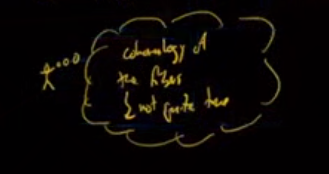
\includegraphics[width=3.64583in,height=\textheight]{figures/image_2020-12-28-18-24-08.png}
\caption{Cohomology of the fibers: but not quite!}
\end{figure}

This is not quite true, and the obstruction is called \textbf{the base
change property}, which we'll see later in the course. What's true in
general is that \(R^i f_* \mathcal{F}\) is the sheafification of the
presheaf \(V\to H^i(f^{-1}(V), \mathcal{F})\), which is not quite the
cohomology of the fibers since sheafification is somewhat brutal.

\begin{proposition}[Derived pushforwards for finite morphisms]

If \(f\) is a finite morphism (e.g.~a closed immersion) then
\(R^{>0} f_* = 0\).

\end{proposition}

\begin{exercise}[Proof, must-do!]

Prove this. The claim is that \(f_*\) is right-exact, which in this case
shows it is exact. Check on stalks. Compute that the stalk of
\(f_* \mathcal{F}\) at
\(\mkern 1.5mu\overline{\mkern-1.5muy\mkern-1.5mu}\mkern 1.5mu\in Y\) is
given by
\begin{align*}
f_* \mathcal{F}_{\mkern 1.5mu\overline{\mkern-1.5muy\mkern-1.5mu}\mkern 1.5mu} = \bigoplus_{\mkern 1.5mu\overline{\mkern-1.5mux\mkern-1.5mu}\mkern 1.5mu\in f^{-1}(\mkern 1.5mu\overline{\mkern-1.5muy\mkern-1.5mu}\mkern 1.5mu)}\mathcal{F}_{\mkern 1.5mu\overline{\mkern-1.5mux\mkern-1.5mu}\mkern 1.5mu}
\end{align*}
for \(f\) a finite morphism (not necessarily unramified).

\end{exercise}

\begin{proposition}[technical]

\(f_*\) preserves injectives.

\end{proposition}

\begin{exercise}[proof]

Prove this! You can do this by showing the following fact from category
theory: this is true for any functor with an exact left adjoint, which
here is \(f^*\) and is exact since filtered colimits and sheafification
are both exact, or alternatively you can check on stalks, since the
stalks of \(f^{-1}\) are the stalks of the original functor.

\end{exercise}

\begin{corollary}[The Leray Spectral Sequence]

Suppose \(X \xrightarrow{f} Y\) and \(Y \xrightarrow{g} Z\) are
morphisms of schemes, then there is a spectral sequence
\begin{align*}  
R^i g_* R^j f_* \mathcal{F} \Rightarrow R^{i+j}(g\circ f)_* \mathcal{F}
.\end{align*}
As a special case, for \(Z = \operatorname{Spec}k\) with
\(k=\mkern 1.5mu\overline{\mkern-1.5muk\mkern-1.5mu}\mkern 1.5mu\), then
\(g_*, f_*\) are taking global sections so we get
\begin{align*}  
H^i(Y, R^j f_* \mathcal{F} ) \Rightarrow H^{i+j}(X, \mathcal{F})
.\end{align*}

\end{corollary}

\begin{proof}[sketch]

There is a general statement (see Tohoku): given two functors between
abelian functors where the first preserves injectives, you get such a
spectral sequence. How to explicitly compute this: we can take an
injective resolution \(\mathcal{F}\to \mathcal{I}^{\,\cdot\,}\) and
compute
\begin{align*}  
R^i f_* \mathcal{F} \mathcal{H}^i(f_* \mathcal{I}^{\,\cdot\,})
.\end{align*}
\(f_* \mathcal{I}\) is a complex of injectives, and we want
\(\mathcal{H}^{i+j}(g_* f_* \mathcal{I}^{\,\cdot\,}) = R^{i+j}(g\circ f)_* \mathcal{F}\),
and the content here is that we don't have to take an additional
injective resolution of \(f_* \mathcal{I}\). Now take the spectral
sequence of the filtered complex \(f_* \mathcal{I}^{\,\cdot\,}\) where
the filtration is by the truncations
\(\tau_{\leq p}f_* \mathcal{I}^{\,\cdot\,}\) where you replace the
\(p\)th term with the kernel of the differential and zero beyond this
point. An example of a differential is given by the following: there are
SESs
\begin{align*}  
0 \to
\tau_{\leq p} f_* \mathcal{I}^{\,\cdot\,}
\to
\tau_{\leq p+1} f_* \mathcal{I}^{\,\cdot\,}
\to
\mathcal{H}^{p+1}(f_* \mathcal{I}^{\,\cdot\,})  = R^{p+1} f_* \mathcal{F}
\to 
0
,\end{align*}
and applying \(RG_*\) yields a map
\begin{align*}  
R^{p+1} f_* \mathcal{F}
\xrightarrow{\delta}
R^{q+1} g_* \tau_{\leq p}f_* \mathcal{I}^{\,\cdot\,}
,\end{align*}
and after some splicing this \(\delta\) will be the differential on
\(E_2\).

\end{proof}

Next time: the Brauer group.

\hypertarget{lecture-11}{%
\section{Lecture 11}\label{lecture-11}}

\hypertarget{pushforwards-continued}{%
\subsection{Pushforwards (Continued)}\label{pushforwards-continued}}

Last time: we saw the Leray spectral sequence, but no examples yet, so
that's what we'll do now. We had
\(X \xrightarrow{f} Y \xrightarrow{g} Z\) to which we associated the
spectral sequence
\(R^i f_* R^jf_*({\,\cdot\,}) \Rightarrow R^{i+j}(g\circ f)_* ({\,\cdot\,})\).
To deduce existence we used that pushforwards preserve injectives, and
we looked at some \(E_2\) differentials.

\begin{example}[?]

Let \(X \xrightarrow{\pi} Z \coloneqq\operatorname{Spec}k\), where
\(k\neq \mkern 1.5mu\overline{\mkern-1.5muk\mkern-1.5mu}\mkern 1.5mu\)
necessarily. The spectral sequence for the functors \(\pi_*, \Gamma\)
yields the Leray spectral sequence
\(H^i(k, R^j \pi_* \mathcal{F}) \Rightarrow H^{i+j}(X_\text{ét}, \mathcal{F})\).
The LHS is the étale cohomology of \(\operatorname{Spec}k\), i.e.~Galois
cohomology. The Galois module corresponding to \(R^j \pi_* \mathcal{F}\)
is \(H^j(X_{k^{s}}, \mathcal{F})\) by taking the
\(\mkern 1.5mu\overline{\mkern-1.5muk\mkern-1.5mu}\mkern 1.5mu\) points
of this functor So the Leray spectral sequence yields
\begin{align*}  
H^i(k, H^j(X_{k^{s}, \text{ét}}, \mathcal{F} )) \Rightarrow H^{i+j}(X_\text{ét}, \mathcal{F})
.\end{align*}

Consider \(k\) a finite field and \(X_{/k}\) a smooth projective
variety. Then the Galois cohomology is given by
\begin{align*}  
H^i(k, V) 
=
\begin{cases}
V^G & i = 0 \hspace{4em}\text{the invariants}\\
V_G & i = 1\hspace{4em}\text{the coinvariants} \\
0 & i>1
\end{cases}
\end{align*}
This follows from computing the cohomology of
\(\widehat{{\mathbb{Z}}}\). Supposing we knew that the cohomological
dimension of a smooth projective variety was \(2n\) over
\(\mkern 1.5mu\overline{\mkern-1.5muk\mkern-1.5mu}\mkern 1.5mu\)
(e.g.~taking \(\mathcal{F} \coloneqq\mathbb{Z}/\ell\mathbb{Z}\) above),
then the cohomological dimension of \(X\) would be \(2n+1\). This
follows from \(E_2\) vanishing for \(i>1\) in this case.

\end{example}

\begin{remark}

A general fact about the Leray spectral sequence for smooth proper
morphisms: let \(X \xrightarrow{\pi} Y\) such a morphism, then there is
a spectral sequence
\begin{align*}  
H^i(Y, R^j \pi_* \underline{{\mathbb{Q}}}) \Rightarrow H^{i+j}(X, {\mathbb{Q}})
.\end{align*}
A fact due to Deligne is that this degenerates at \(E_2\), which is
proved with \(\ell{\hbox{-}}\)adic cohomology (going through Weil II)
using the theory of weights. Note that this is false for smooth proper
morphisms between manifolds! Instead, for varieties, they behave more
like products instead of ``twisted'' things.

\end{remark}

\hypertarget{explicit-characterizations}{%
\subsubsection{Explicit
Characterizations}\label{explicit-characterizations}}

We'll now be explicit about what these pushforwards are, so we'll give
another description of them:

\begin{proposition}[?]

Let \(X \xrightarrow{\pi} Y\), then \(R^i \pi_* \mathcal{F}\) is the
sheaf associated to the presheaf
\(U\to H^i(\pi^{-1}(U)_\text{ét}, \mathcal{F})\).

\end{proposition}

\begin{proof}[?]

Choose an injective resolution
\(\mathcal{F}\to \mathcal{I}{\,\cdot\,}\), then
\(\mathcal{H}^i(\pi_* \mathcal{I}^{\,\cdot\,}) \coloneqq R^i \pi_* \mathcal{F}\).
Let's compute this pushforward in another way: we have

Here the induced map on presheaves is exact although the forgetful
functor may not be. This is because a sequence of presheaves is exact
iff it's exact on every open, but \(\pi_*\) just pulls back opens. This
diagram commutes since what you get in the top-right corner is already a
sheaf, and sheafification is the identity on sheaves. We can thus factor
\(\pi_*\) to obtain
\begin{align*}  
R^i \pi_* \mathcal{F} = \mathcal{H}^i*\pi_* \mathcal{I}^{\,\cdot\,}
&= \mathcal{H}^i(a\circ \pi \circ f (\mathcal{I}^{\,\cdot\,})) \\
&= a\circ \pi_*\qty{\mathcal{H}^i(f(\mathcal{I}^{\,\cdot\,})) }
.\end{align*}
where we've used the fact that \(\pi_*, s\) are exact. Why isn't the
inner term zero, since \(\mathcal{I}^{\,\cdot\,}\) is an exact complex
of sheaves? Epimorphisms are different in the categories of sheaves and
presheaves, so it may not be exact when viewed as a complex of
presheaves. These terms are explicitly the functors
\(U\to H^i(U, \mathcal{F})\), since
\({ \left.{{\mathcal{I}^{\,\cdot\,}}} \right|_{{U}} }\) is an injective
resolution of \(\mathcal{F}\). We can now evaluate this on an open of
\(Y\), so we get
\begin{align*}  
a \qty{ (U \xrightarrow{\text{ét}} Y) \to H^i(\pi^{-1}(U), \mathcal{F}) }
,\end{align*}
which is sheafifying the functor we want.

\hypertarget{explicit-characterizations-1}{%
\subsubsection{Explicit
Characterizations}\label{explicit-characterizations-1}}

\end{proof}

\begin{example}[?]

Suppose \(X\) is an integral scheme and
\(\eta\xhookrightarrow{\iota} X\) is its generic point. Suppose
\(\mathcal{F}\in {\operatorname{Sh}}(\eta_\text{ét})\). How to we
understand \(R^i \iota_* \mathcal{F}\)? We can compute its stalks:
suppose
\(\mkern 1.5mu\overline{\mkern-1.5mux\mkern-1.5mu}\mkern 1.5mu \to X\)
is a geometric point, then
\begin{align*}  
\qty{R^i \iota_* \mathcal{F}}_{\mkern 1.5mu\overline{\mkern-1.5mux\mkern-1.5mu}\mkern 1.5mu} 
&= 
\varinjlim_{(U, \mkern 1.5mu\overline{\mkern-1.5muu\mkern-1.5mu}\mkern 1.5mu)} \qty{R^i \iota_* \mathcal{F}}(U) \\
&=
H^i(U_\eta, { \left.{{\mathcal{F}}} \right|_{{U_\eta}} })
.\end{align*}
where we take limits over \(U\xrightarrow{\text{ét}} X\) and
\(\mkern 1.5mu\overline{\mkern-1.5muu\mkern-1.5mu}\mkern 1.5mu\to U\) is
a geometric point above
\(\mkern 1.5mu\overline{\mkern-1.5mux\mkern-1.5mu}\mkern 1.5mu\).

\begin{exercise}[Important, must-do]

Let
\({\mathcal{O}}_{X, \mkern 1.5mu\overline{\mkern-1.5mux\mkern-1.5mu}\mkern 1.5mu}\)\footnote{The
  \textbf{strictly Henselian ring} of \(X\) at
  \(\mkern 1.5mu\overline{\mkern-1.5mux\mkern-1.5mu}\mkern 1.5mu\).} be
the stalk of \({\mathcal{O}}_X\) at
\(\mkern 1.5mu\overline{\mkern-1.5mux\mkern-1.5mu}\mkern 1.5mu\) and
\(K_{\mkern 1.5mu\overline{\mkern-1.5mux\mkern-1.5mu}\mkern 1.5mu}\)\footnote{The
  \textbf{strictly Henselian field} of \(X\) at
  \(\mkern 1.5mu\overline{\mkern-1.5mux\mkern-1.5mu}\mkern 1.5mu\).} be
its fraction field. Then
\begin{align*}  
\qty{R^i \iota_* \mathcal{F}}_{\mkern 1.5mu\overline{\mkern-1.5mux\mkern-1.5mu}\mkern 1.5mu}
=
H^i(K_{\mkern 1.5mu\overline{\mkern-1.5mux\mkern-1.5mu}\mkern 1.5mu}, { \left.{{\mathcal{F}}} \right|_{{K_{\mkern 1.5mu\overline{\mkern-1.5mux\mkern-1.5mu}\mkern 1.5mu}}} } )
,\end{align*}
where the RHS is either the Galois cohomology of \(k\) or the étale
cohomology of \(\operatorname{Spec}k\).

Idea: these are the étale local rings, and this says you can compute the
stalk of a cohomology sheaf in terms of these strictly Henselian local
rings.

\end{exercise}

\end{example}

\hypertarget{uxe9tale-cohomology-of-curves-reducing-to-galois-cohomology}{%
\subsection{Étale Cohomology of Curves: Reducing to Galois
Cohomology}\label{uxe9tale-cohomology-of-curves-reducing-to-galois-cohomology}}

Goal: we want to understand \(H^{>1}(X, {\mathbb{G}}_m)\) where
\(X_{/k}\) is a curve over \(k = k^{s}\) which is separably closed.
We'll reduce this to questions in Galois cohomology.

\begin{proposition}[?]

Let \(X_{/k}\) (with \(k\) not necessarily algebraically closed) be a
regular (integral) variety and \(\eta\hookrightarrow X\) is the generic
point. Then there is a SES in \({\operatorname{Sh}}(X_\text{ét})\):
\begin{align*}  
0 \to
{\mathbb{G}}_m
\xrightarrow{\operatorname{Res}}
\eta_* {\mathbb{G}}_m 
\xrightarrow{\operatorname{Div}}
\bigoplus_{z\in X, \operatorname{codim}1} \iota_{z_*} \underline{{\mathbb{Z}}}
\to 0
,\end{align*}
where the middle term can be thought of as pushing forward
\({\mathbb{G}}_m\) from the étale site of \(\eta\) or pulling back
\({\mathbb{G}}_m\) to it, which is just \({\mathbb{G}}_m\) again, and
pushing forward again, and the last term is the \textbf{sheaf of
divisors}.

\end{proposition}

\begin{remark}

The first map is either the unit or the counit of the adjunction
\(\eta_* \rightleftharpoons\eta^*\), which is the restriction. The
second map comes from noting that on an étale morphism \(U\to X\), this
is a bunch of rational functions and you can take its divisor. This
gives a number for each codimension 1 point: the order of vanishing. All
but finitely many numbers will be zero, so you get a section to the last
sheaf.

\end{remark}

\begin{proof}[of exactness]

\textbf{1}: \({\mathbb{G}}_m \to \eta_* {\mathbb{G}}_m\) is injective.
This reduces to showing \({\mathbb{G}}_m(U) \to {\mathbb{G}}_m(U_\eta)\)
is injective, where \(U_\eta\) is the fiber over \(\eta\), since this is
\({\mathcal{O}}_U^{\times}\to \bigoplus_{\eta_i} {\mathcal{O}}_{\eta_i}\)
which is a sum over generic points of \(U\). This uses that \(X\) is
reduced.

\textbf{2}: Exactness in the middle. Given
\(f\in \eta_* {\mathbb{G}}_m(U)\) with \(\operatorname{Div}(f) = 0\), we
want to show \(f\) comes from \({\mathbb{G}}_m(U)\). We need to show
\(f, f^{-1}\) are regular, and it's enough to show that \(f\) is
regular. We're using that if we have a finite type ring over a field
\(A\), then by a fact from commutative algebra,
\begin{align*}
A = \bigcap_{\mathfrak{p}\in \operatorname{Spec}^1(A)} A_{\mathfrak{p}}
\end{align*}
which is the intersection of localizations over all height 1 primes.
Being in this intersection is equivalent to having non-negative
divisors, where here we've used that regularity implies normality.

\textbf{3}: Surjectivity at the end. We need to show that every divisor
is étale locally principle, and thus Zariski locally. A global section
to the last sheaf is a Weil divisor, and we want to show each is
principle. This is equivalent to being Cartier, which is true here by
regularity.

\end{proof}

\begin{corollary}[?]

There's a LES:

The blue term is what we'd like to compute, and the other terms are the
cohomology of pushforwards and thus appear in the Leray spectral
sequence.

\end{corollary}

\begin{proposition}[?]

Let \(X_{/k}\) be a curve where \(k=k^{s}\). Then
\begin{align*}  
H^{i>0}(X_\text{ét}, \bigoplus_{\operatorname{codim}z = 1} \iota_{z_*} {\mathbb{Z}}) = 0
.\end{align*}

\end{proposition}

\begin{proof}[?]

It's enough to show that
\(H^{>0}(X_\text{ét}, \iota_{z_*} \underline{{\mathbb{Z}}}) = 0\) using
that cohomology commutes with direct sums. Using the Leray spectral
sequence, we get
\begin{align*}
H^i(X_\text{ét}, R^j_{\iota_{z_*}} \underline{{\mathbb{Z}}})\Rightarrow H^{i+j}(z_\text{ét}, \underline{{\mathbb{Z}}})
\end{align*}
What are the coefficients on the LHS? We proved that pushforwards on
closed immersions are exact, by checking on stalks, so we have

\begin{align*}  
R^j _{\iota_{z_*}} \underline{{\mathbb{Z}}}
=
\begin{cases}
\iota_{z_*} \underline{{\mathbb{Z}}}& j = 0 \\
0 & j > 0
\end{cases}
.\end{align*}

We can also compute
\begin{align*}  
H^s(z_\text{ét}, \underline{{\mathbb{Z}}})
=
\begin{cases}
{\mathbb{Z}}& s = 0 \\
0 & s>0
\end{cases}
.\end{align*}
since the zero term is global sections and \(k\) is separably
(algebraically) closed, and the Galois cohomology vanishes in \(i>0\).
So we get a degenerate spectral sequence with one column, yielding
\begin{align*}  
H^i (X_\text{ét}, \iota_{z_*} \underline{{\mathbb{Z}}}) 
=
H^i(z_{\text{ét}}, {\mathbb{Z}})
=
\begin{cases}
{\mathbb{Z}}& i = 0 \\
0 & i> 0
\end{cases}
.\end{align*}

\end{proof}

\begin{corollary}[?]

If \(X_{/k}\) is a smooth curve over \(k=k^{s}\) then we have an
isomorphism
\begin{align*}  
H^{>1}(X_\text{ét}, {\mathbb{G}}_m) \xrightarrow{\sim}H^{>i}(X_\text{ét}, \eta_* {\mathbb{G}}_m)
.\end{align*}

\end{corollary}

New goal: compute the RHS, which is not quite Galois cohomology but is
pushed forward from a field. Using the Leray spectral sequence, we get
\begin{align*}  
H^i(X_\text{ét}, R^j \eta_* {\mathbb{G}}_m)
\Rightarrow
H^{i+j}(\eta, {\mathbb{G}}_m)
,\end{align*}
where the RHS is Galois cohomology. We're interested in the \(j=0\)
region of the spectral sequence. Let's try to understand the stalks at
geometric points:
\begin{align*}  
\qty{R^j \eta_* {\mathbb{G}}_m}_{\mkern 1.5mu\overline{\mkern-1.5mux\mkern-1.5mu}\mkern 1.5mu}
=
H^j(K_{\mkern 1.5mu\overline{\mkern-1.5mux\mkern-1.5mu}\mkern 1.5mu}, {\mathbb{G}}_m)
,\end{align*}
where the field appearing is the \emph{strict Henselization} from the
earlier discussion. We'll be able to compute this if we have the
following theorem:

\begin{theorem}[?]

Let \(K\) be the function field of a curve or an algebraically closed
field, or
\(K = K_{\mkern 1.5mu\overline{\mkern-1.5mux\mkern-1.5mu}\mkern 1.5mu}\)
is the strict Henselian field of a geometric point of a curve over a
separably (algebraically) closed field. Then
\begin{align*}  
H^{>0}(K, {\mathbb{G}}_m) = 0
.\end{align*}

\end{theorem}

This will suffice since \(R^{>0} \eta_*{\mathbb{G}}_m = 0\), yielding a
spectral sequence where \(E_2 = E_ \infty\):
\begin{align*}  
H^i(X_\text{ét}, \eta_* {\mathbb{G}}_m)
=
H^i(\eta,{\mathbb{G}}_m)
=
0 && \text{if }i>0
.\end{align*}

\textbf{Upshot}: this reduces the computation of the étale cohomology of
a curve to Galois cohomology. Proving this theorem is hard, and will
lead us to Brauer groups.\footnote{Another one of Daniel's favorite
  topics in the course!}

\hypertarget{brauer-groups}{%
\subsection{Brauer Groups}\label{brauer-groups}}

\begin{definition}[Cohomological Brauer Group]

Let \(X\) be a scheme, then the \textbf{cohomological Brauer group} is
defined as
\begin{align*}  
\operatorname{Br}(X) \coloneqq H^2(X_\text{ét}, {\mathbb{G}}_m)_{{\operatorname{tors}}}
.\end{align*}

\end{definition}

In good situations, this group has a good geometric interpretation, so
let's true to understand it this way in terms of
\(\operatorname{PGL}_n{\hbox{-}}\)torsors.

\begin{claim}

There is a natural map
\begin{align*}  
\bigcup_n \left\{{ \text{étale-locally split $\operatorname{PGL}_n{\hbox{-}}$torsors} }\right\}
\to
H^2(X_\text{ét}, {\mathbb{G}}_m)
.\end{align*}

\end{claim}

Idea: there is a SES
\begin{align*}  
1 \to {\mathbb{G}}_m \to \operatorname{GL}_n \to \operatorname{PGL}_n \to 1
&& \in {\operatorname{Sh}}^{{\operatorname{Grp}}}(X_\text{ét})
.\end{align*}
It's not obviously exact on the right, since it's not quite true that a
map into \(\operatorname{PGL}_n\) is an invertible matrix modulo
scaling: this is true locally, but it's the \emph{sheafification} of
this, so why is there a surjection? The key input is that
\(\operatorname{GL}_n\to \operatorname{PGL}_n\) is smooth, and thus has
sections étale-locally. This map is a
\({\mathbb{G}}_m{\hbox{-}}\)torsor, which we know are Zariski-locally
trivially, so this sequence is exact in the Zariski topology and thus
also in the étale topology.

Suppose \(T\) is an étale-locally trivial
\(\operatorname{PGL}_n{\hbox{-}}\)torsor, then the LES essentially has
the following map:
\begin{align*}  
\cdots \to H^2(X_\text{ét}, \operatorname{PGL}_n) \xrightarrow{\delta} H^2(X_\text{ét}, {\mathbb{G}}_m) \to \cdots
.\end{align*}
This doesn't make sense \emph{a priori} since this is not a sequence of
abelian sheaves. Let's true to associate to \(T\) some
\([T]\in H^2(X_\text{ét}, {\mathbb{G}}_m)\). We can first write down
\([T] \in {\check{H}}^1(X_\text{ét}, \operatorname{PGL}_n)\): we get a
\(\operatorname{PGL}_n\) cocycle out a torsor by choosing a trivializing
map \(U\to X\) so that
\({ \left.{{T}} \right|_{{U}} } = { \left.{{\operatorname{PGL}_n}} \right|_{{U}} }\).
This yields a cocycle in \(\operatorname{PGL}_n(U\times_X U)\).

\begin{quote}
To be continued.
\end{quote}

\hypertarget{lecture-12}{%
\section{Lecture 12}\label{lecture-12}}

\hypertarget{brauer-groups-1}{%
\subsection{Brauer Groups}\label{brauer-groups-1}}

Goal: for \(C\) a curve over
\(k=\mkern 1.5mu\overline{\mkern-1.5muk\mkern-1.5mu}\mkern 1.5mu\),
we've computed
\begin{align*} 
H^i(C, {\mathbb{G}}_m) 
= 
\begin{cases}
{\mathcal{O}}_C^{\times}(C) & i=0\\
{\operatorname{Pic}}(C) & i=1 \\
0 & i > 1
\end{cases}
.\end{align*}
Currently \(i>1\) is a mystery, so today we'll look at \(i=2\). Recall
that we've reduced this to the Galois cohomology of the function field
\(H^i(k(C), {\mathbb{G}}_m)\) and of the strict Henselization
\footnote{The stalk of the structure sheaf, \({\mathcal{O}}_{C,x}\).}
\(H^i(K_{\mkern 1.5mu\overline{\mkern-1.5mux\mkern-1.5mu}\mkern 1.5mu}, {\mathbb{G}}_m)\).

Today we'll try to understand the Galois cohomology of a field with
coefficient in
\(\mkern 1.5mu\overline{\mkern-1.5muk\mkern-1.5mu}\mkern 1.5mu^{\times}\),
or \({\mathbb{G}}_m\) thought of as a sheaf on the étale site. We'll
discuss \(i=2\), and a general principle in group cohomology is that if
one understands \(i=1, 2\) then one can often understand all degrees.

In general, \(H^1\) has a geometric interpretation: torsors. \(H^2\) is
much harder: they classify more general objects called \textbf{gerbes}.
A miracle is that \(H^2({\mathbb{G}}_m)\) has real meaning, and is very
closely related to real physical objects (certain torsors). Recall that
we defined the \emph{cohomological Brauer group of \(X\)}
(\cref{def:cohom_brauer_group}) as
\begin{align*}  
\operatorname{Br}^{\operatorname{coh}}\coloneqq\operatorname{Br}'(X) \coloneqq H^i(X_\text{ét}, {\mathbb{G}}_m)_{{\operatorname{tors}}}
.\end{align*}

We also started defining the Brauer group by considering
\begin{align*}  
\bigcup_n \left\{{\text{étale locally trivial } \operatorname{PGL}_n{\hbox{-}}\text{torsors}}\right\}
\xrightarrow{\delta}
H^2(X_\text{ét}, {\mathbb{G}}_m)
,\end{align*}
and defining \(\operatorname{Br}(X) \coloneqq\operatorname{im}f\) as a
set, which is a reasonably concrete geometric object. This map came from
a LES in cohomology, coming from a SES of sheaves, not all of which were
abelian. The definition of \(\delta\) was the boundary map of
\begin{align*}  
\bigcup_n H^1(X_\text{ét}, \operatorname{PGL}_n)
\xrightarrow{\delta}
H^2(X_\text{ét}, {\mathbb{G}}_m)
\label{eq:12_union_1}
\end{align*}
arising from the SES of sheaves of groups on \(X_\text{ét}\),
\begin{align*}  
1 
\to {\mathbb{G}}_m 
\xrightarrow{} 
\operatorname{GL}_m
\xrightarrow{}
\operatorname{PGL}_n \to 1
.\end{align*}
We argued last time that this was exact in the Zariski topology since
the RHS map was a \({\mathbb{G}}_m{\hbox{-}}\) torsor and thus Zariski
locally trivial. What does \(\delta\) mean? \footnote{Best reference:
  Giraud, ``Cohomologie non Abelienne''.}

\begin{remark}

Making the LES here is a little subtle. You get a long exact sequence of
\emph{sets} here which terminates at the \(H^2\) we're interested in,
although one usually doesn't get a map of the form \(H^1(C) \to H^2(B)\)
for a SES \(A \xrightarrow{}B \xrightarrow{}C\), you need that \(A\) is
abelian (or in the center).

\end{remark}

We'll now try to make \(\delta\) explicit in terms of Čech cohomology,
which is the only way we have to make sense of the LHS set in
\cref{eq:12_union_1}. We defined it to be the set of étale locally
trivial \(\operatorname{PGL}_n{\hbox{-}}\) torsors, which has a
description in terms of \({\check{H}}^1\) : the boundary map doesn't
usually make sense for a nonabelian group, but it does in very low
degrees such as \(i=1\). So we need to implement the snake lemma. Start
with \([T]\in H^i(X_\text{ét}, \operatorname{PGL}_n)\) where \(T\) is a
\(\operatorname{PGL}_n{\hbox{-}}\) torsor split by \(U\xrightarrow{}X\).
On \(U\times_X U\), descent data is given by a section
\(\Gamma(U\times_X U, \operatorname{PGL}_n)\) as a sheaf. This is
because descent data is an isomorphism on this double intersection and
an automorphism of \(\operatorname{PGL}_n\) is the same as a section to
\(\operatorname{PGL}_n\). This descent data satisfies the cocycle
condition. How do we apply the boundary map to an element in the Čech
complex? After refining \(U\) we can lift this descent data to a section
\(s\in \Gamma\qty{U\times_{X}U,GL_{n}}\). Note that
\(H^{2}\qty{{\mathbb{G}}_{m}}\) is represented by a section to
\({\mathbb{G}}_{m}\) of \(U\times_{X}U\times_{X}U\). We started with
something satisfying the cocycle condition but lifted in an arbitrary
way, so it may not still satisfy the cocycle condition. We can write
\begin{align*}  
\pi_{23}^{*}\pi_{12}^{*}s \qty{\pi_{13}s}^{-1}
\in \Gamma\qty{U\times_{X}U\times_{X}U, {\mathbb{G}}_{m}}
.\end{align*}

A priori it's just a section to \(\operatorname{GL}_{n}\) but we know
that this goes to 1 in \(\operatorname{PGL}_{n}\), meaning it must comes
from \({\mathbb{G}}_{m}\). The LHS is a 2-cocycle representing an
element of \(H^{2}\qty{X_{\text{ét}}, {\mathbb{G}}_{m}}\).

\begin{exercise}[?]

Check that \(d\) of this element is zero.

\end{exercise}

\begin{slogan}

\(\delta\qty{[T]}\) is the obstruction to lifting a
\(\operatorname{PGL}_{n}{\hbox{-}}\)torsor \(T\) to a
\(\operatorname{GL}_{n}{\hbox{-}}\)torsor. If this class vanishes, a
lift exists.

\end{slogan}

\begin{remark}

This is what you might expect: the image of something coming from a
boundary map is the obstruction to coming from the previous map. This
class is called the \textbf{Brauer class of \(T\)}.

\end{remark}

We've just mapped from a set to a group, so we don't know that the image
is a group yet, and we don't yet know that the image is in
\(\operatorname{Br}^{\operatorname{coh}}\) since we don't know if the
image is torsion.

\hypertarget{geometric-interpretations-of-operatornamepgl_nhbox-torsors-brauer-classes}{%
\subsubsection{\texorpdfstring{Geometric Interpretations of
\(\operatorname{PGL}_{n}{\hbox{-}}\)Torsors Brauer
Classes}{Geometric Interpretations of \textbackslash operatorname\{PGL\}\_\{n\}\{\textbackslash hbox\{-\}\}Torsors Brauer Classes}}\label{geometric-interpretations-of-operatornamepgl_nhbox-torsors-brauer-classes}}

There is a general principle: suppose
\(T\in{\operatorname{Sh}}^{{\operatorname{Set}}}\qty{X_{\text{ét}}}\)
and \(G = \underline{{\operatorname{Aut}}}\qty{T}\) as a sheaf, whose
sections are given on an open \(U\) by pulling back \(T\) to \(U\) and
compute its automorphisms, where for example \(T\) is a scheme. There is
a natural bijection

\begin{align*}
\left\{{\substack{\text{ Locally split } \\ G{\hbox{-}}\text{torsors}}}\right\}
&\rightleftharpoons
\left\{{\substack{\text{ forms of  } T}}\right\}
.\end{align*}
An example of this has come up before: namely that
\(\operatorname{GL}_{n}{\hbox{-}}\)torsors corresponded to vector
bundles. This is recovered by taking \(T\) to be the trivial vector
bundle and \(G=\operatorname{GL}_{n}\) Here a \textbf{form} is defined
to be a sheaf on \(X_{\text{ét}}\) locally isomorphic to \(T\). The map
here is given by sending a form \(F\) to
\(\underline{\mathrm{Isom}}\qty{F, T}\). This is locally split since
\(F\) is locally trivial, i.e.~locally isomorphic to \(T\), and so
base-changing to some cover where \(F\) will make this torsor split. The
reverse map is sending \(\tau \to \qty{\tau\times T}/G\), taking the
sheaf quotient, which gets rid of \(\tau\) and making the fibers
isomorphic to \(T\) instead.

\begin{example}[?]

\(\operatorname{GL}_{n}{\hbox{-}}\)torsors correspond to vector bundles.
Note that this isn't an equivalence of categories: there are maps of
vector bundles which don't come from maps of torsors, e.g.~any map that
is not an isomorphism. Here the left/right arrows mean that there is a
bijection between \emph{sets}, up to isomorphism on each side.

\end{example}

\begin{example}[?]

Let \(G=\operatorname{PGL}_{n}\), then what are objects with
automorphism group
\({\operatorname{Aut}}\qty{G} = \operatorname{PGL}_{n}\)? An example
that works here is
\({\operatorname{Aut}}_{x}\qty{{\mathbb{P}}_{x}} = \operatorname{PGL}_{n}\).

\end{example}

\begin{exercise}[?]

You may have seen this stated over an algebraically closed based field,
but (nontrivially) this holds over a general base. Prove this.

\emph{(Hint: you may need to use the theorem on formal functions or
formal GAGA.)}

\end{exercise}

\begin{corollary}[?]

There is a natural bijection
\begin{align*}
\left\{{\substack{\operatorname{PGL}_{n}{\hbox{-}}\text{torsors}}}\right\}
&\rightleftharpoons
\left\{{\substack{\text{Forms of } {\mathbb{P}}^{n-1}}}\right\}
\end{align*}
These are referred to as \textbf{Severi-Brauer \(X{\hbox{-}}\)Schemes}
\footnote{If \(x = \operatorname{Spec}k\) is a point, then these are
  referred to as \textbf{Severi-Brauer Varieties}.} .

\end{corollary}

\begin{example}[?]

The algebra \(A\coloneqq\operatorname{Mat}_{n\times n}\) has
\({\operatorname{Aut}}(A) = \operatorname{PGL}_{n}\), which is usually
referred to as the \emph{Noether-Skolem} theorem. Thus there is a
bijection
\begin{align*}
\left\{{\substack{\operatorname{PGL}_n{\hbox{-}}\text{torsors}}}\right\}
&\rightleftharpoons
\left\{{\substack{\text{Forms of } \operatorname{Mat}_{n\times n} = \operatorname{End}_{{\mathcal{O}}_{x}} ({\mathcal{O}}_{x}^{n})}}\right\}
\end{align*}
The RHS are referred to as \textbf{Azumaya algebras}, and over a field
these are central simple algebras. There is a fact (which we may see)
that such algebras over a field are always division algebras.

\end{example}

\begin{question}

How can we combine these to send forms of \({\mathbb{P}}^{n-1}\)
directly to an Azumaya algebra?

\end{question}

\begin{remark}

Key takeaway: the Brauer group (which we'll soon prove is a group) has
concrete representative. These are the forms of \({\mathbb{P}}^{n-1}\),
which you can think of as étale locally trivial \({\mathbb{P}}^{n-1}\)
bundles, or forms of a matrix algebra, i.e.~coherent sheaves of algebras
which étale locally endomorphisms of the trivial bundle.

\end{remark}

\hypertarget{twisted-sheaves}{%
\subsection{Twisted Sheaves}\label{twisted-sheaves}}

People usually think about Brauer groups as one of these two objects.
We'll discuss a third way. When we defined the boundary map, we took
descent data from \(\operatorname{PGL}_n\), i.e.~elements of this group
on double intersections, and we lifted those to
\(\operatorname{GL}_{n}\).

\begin{definition}[Twisted Sheaves]

Let \(U \to X\) be an étale cover and suppose
\(\alpha \in \Gamma(U \times_{X} U \times_{X} U, {\mathbb{G}}_{m})\)
represents \([\alpha] \in H^{s}i(X_{\text{ét}}, {\mathbb{G}}_{m})\).
Then an \textbf{\(\alpha{\hbox{-}}\)twisted sheaf} is a quasicoherent
sheaf on \(U\), an isomorphism
\(\varphi:\pi_{1}^{*} \mathcal{F} \xrightarrow{\sim}\pi_{2}^{*} \mathcal{F}\)
(which looks like descent data) which satisfies the cocycle condition up
to \(\alpha\), i.e.~
\begin{align*}  
\pi_{23}^{*} \phi \circ \pi_{12}^{*}\phi = \alpha \pi_{13}^{*}\phi
.\end{align*}

\end{definition}

\begin{remark}

Note that if \(\alpha\) were the constant function 1, this would be the
descent data for a quasicoherent sheaf, so we're twisting what it means
to be a sheaf. This is exactly what we did when defining a
\(\operatorname{PGL}_{n}{\hbox{-}}\)torsor, where we lifted to get
isomorphisms between the \(\operatorname{GL}_{n}\) sheaves on the double
overlaps. These failed to satisfy the cocycle condition, and the Brauer
class measured this failure. So in defining \(\delta\), our intermediate
step was a twisted sheaf.

\end{remark}

So we'll define the category \({\mathrm{QCoh}}(X, \alpha)\) whose
objects are \(\alpha{\hbox{-}}\)twisted sheaves and whose morphisms are
morphisms of sheaves on \(U\) commuting with \(\varphi\).

\begin{example}[?]

\({\mathrm{QCoh}}(X, 1)\) is canonically isomorphic to
\({\mathrm{QCoh}}(X)\), which is the very famous theorem of \emph{étale
descent}.

\end{example}

\hypertarget{categorical-properties}{%
\subsubsection{Categorical Properties}\label{categorical-properties}}

\begin{proposition}[?]

Let \(\alpha, \alpha'\) be two cocycles for \({\mathbb{G}}_{m}\). Then

\begin{enumerate}
\def\labelenumi{\arabic{enumi}.}
\item
  \([\alpha]\in\operatorname{Br}(X)\) (so its in the image the boundary
  map from \(\operatorname{PGL}_{n}\)) iff there exist a twisted vector
  bundle.\footnote{Note that we've proved this already since
    \(\operatorname{Br}= \operatorname{im}\delta\), but part of our
    construction of \(\delta\) involved constructing an
    \(\alpha{\hbox{-}}\)twisted sheaf out of a
    \(\operatorname{PGL}_{n}{\hbox{-}}\)torsor.}
\item
  \({\mathrm{QCoh}}(X,\alpha)\) is an abelian category (easy) and has
  enough injectives (hard) is \(X\) is ``nice''.
\item
  There is a functor
  \begin{align*}  
  \otimes: {\mathrm{QCoh}}(X, \alpha) \times{\mathrm{QCoh}}(X, \alpha') \xrightarrow{} {\mathrm{QCoh}}(X, \alpha \alpha')
  ,\end{align*}
  where is \(\alpha,\alpha'\) are defined on different covers than one
  passes to a common refinement, and a functor\footnote{This and the
    tensor functor come from homming (resp. tensoring) the sheaves
    together and using the pseudo descent data.}
  \begin{align*}  
  \hom: {\mathrm{QCoh}}(X, \alpha) \times{\mathrm{QCoh}}(X, \alpha') \xrightarrow{} 
  {\mathrm{QCoh}}(X, \alpha' \alpha^{-1})
  .\end{align*}
\item
  There are functors
\end{enumerate}

\begin{align*}  
\operatorname{Sym}^{n}, \Lambda^{n} \xrightarrow{} {\mathrm{QCoh}}(X, \alpha) \xrightarrow{} {\mathrm{QCoh}}(X, n \alpha)
.\end{align*}

\begin{enumerate}
\def\labelenumi{\arabic{enumi}.}
\setcounter{enumi}{4}
\tightlist
\item
  \({\mathrm{QCoh}}(X, q) \xrightarrow{\sim}{\mathrm{QCoh}}(X)\).
\end{enumerate}

\end{proposition}

\begin{proof}[Sketch/Discussion]

\envlist

For (1), if \(\alpha\in \operatorname{Br}(X)\), then there is
\(\operatorname{PGL}_{n}{\hbox{-}}\)torsor whose boundary is \(\alpha\),
and our construction of \(\delta\) yielded an
\(\alpha{\hbox{-}}\)twisted vector bundle. Given such a bundle, one can
obtain a Brauer class by constructing a twisted form a
\({\mathbb{P}}^{n}\): take the projectivization. Then the quasi descent
data becomes actual descent data since the failure was precisely in
scalars, which you're now modding out by.

For (3), just work out what happens to \(\alpha, \alpha'\) when
tensoring or homming. Similarly, all of the rest except for \textbf{(2)}
follow from definitions.

\end{proof}

\begin{exercise}[?]

Try to prove (3) and (4).

\end{exercise}

\hypertarget{the-brauer-group-is-a-group}{%
\subsubsection{The Brauer Group is a
Group}\label{the-brauer-group-is-a-group}}

\begin{corollary}[?]

\(\operatorname{Br}(X)\) is a group.

\end{corollary}

\begin{proof}[?]

Let \(\mathcal{E}, \mathcal{E}'\) be \(\alpha,\alpha'{\hbox{-}}\)twisted
vector bundles respectively, we want to show that there exists an
\(\alpha\alpha'{\hbox{-}}\)twisted vector bundle. We can take
\(\mathcal{E}\otimes\mathcal{E}'\), and then just note that having a
twisted vector bundle is the same as having a Brauer class. For
inverses, suppose \(\alpha\) is a Brauer class and \(\mathcal{E}\) is a
twisted vector bundle. To get an \(\alpha^{-1}{\hbox{-}}\)twisted vector
bundle, one can just take the dual \(\mathcal{E}^\vee\).

\end{proof}

\hypertarget{results-on-twisted-bundles}{%
\subsection{Results On Twisted
Bundles}\label{results-on-twisted-bundles}}

\begin{proposition}[?]

Suppose that \(\alpha\) is a 2-cocycle for \({\mathbb{G}}_{m}\), then
\([\alpha]\) is trivial iff there exists an \(\alpha{\hbox{-}}\)twisted
line bundle.

\end{proposition}

\begin{lemma}[?]

If \([\alpha] = [\alpha']\), then
\({\mathrm{QCoh}}(X,\alpha) \simeq {\mathrm{QCoh}}(X, \alpha')\).

\end{lemma}

Note that this is not a canonical equivalence.

\begin{exercise}[?]

Prove this lemma.

\end{exercise}

\begin{proof}[of proposition, $\implies$]

If \(\alpha\) is trivial, then \([\alpha] = [1]\) in which case
\({\mathrm{QCoh}}(X,\alpha) \simeq {\mathrm{QCoh}}(X)\) are equivalent
categories and \({\mathcal{O}}_{X}\) is an honest line bundle.

\end{proof}

\begin{proof}[$\impliedby$]

Suppose you have an \(\alpha{\hbox{-}}\)twisted line bundle. Then
writing down a line bundle is done by taking a cover, taking the trivial
bundle on each open, and then the double intersections have gluing data
in the form of \(s\in \Gamma({\mathbb{G}}_{m})\). To prove \(\alpha\) is
a trivial Brauer class, note that the descent data (gluing data) is the
same as a section \(\beta\in \Gamma(U \times_{X} U, {\mathbb{G}}_{m})\).
Then the Čech differential \(\check{\delta}\) satisfies
\(\check{\delta}(\beta)=\alpha\), and thus by definition
\(\alpha = 0 \in H^{2}({\mathbb{G}}_{m})\).

\end{proof}

\begin{corollary}[?]

Suppose \(\mathcal{E}\) is an \(\alpha{\hbox{-}}\)twisted vector bundle
of rank \(n\). Then \([\alpha]\in H^{2}(X_{\text{ét}}, {\mathbb{G}}_m)\)
is \(n{\hbox{-}}\)torsion.

\end{corollary}

\begin{proof}[?]

We've just proved this for \(n=1\), so for the general case, note that
we can consider \(\Lambda^{n}\mathcal{E}\) is a
\(\alpha^{n}{\hbox{-}}\)twisted line bundle. Then by the previous
proposition, \([\alpha^{n}] - [\alpha]^{n}\) is trivial.

\end{proof}

\begin{corollary}[?]

\begin{align*}  
\operatorname{Br}(X) \subseteq \operatorname{Br}'(X) = H^{2}(X_{\text{ét}}, {\mathbb{G}}_{m})_{{\operatorname{tors}}}
.\end{align*}

\end{corollary}

\hypertarget{examples-of-brauer-classes}{%
\subsubsection{Examples of Brauer
Classes}\label{examples-of-brauer-classes}}

\begin{example}[?]

. \(X\coloneqq\left\{{ x^{2}+y^{2}+z^{2} = 0}\right\}\) over
\({\mathbb{R}}\) is a smooth conic with no rational points. We now via
stereographic projection that a smooth projective conic with a rational
point would be isomorphic to \({\mathbb{P}}^{1}\), so this becomes
isomorphic to \({\mathbb{P}}^{1}\) after base-changing to
\({\mathbb{C}}\) where it does have a rational point. So
\(X_{/{\mathbb{C}}} \cong {\mathbb{P}}^{1}\), which implies that \(X\)
is a twisted form of \({\mathbb{P}}^{1}_{{\mathbb{R}}}\). In fact,
\(\delta\qty{[X]}\) generates
\(\operatorname{Br}({\mathbb{R}}) = {\mathbb{Z}}/2{\mathbb{Z}}\).

\end{example}

\begin{example}[?]

\begin{enumerate}
\def\labelenumi{\arabic{enumi}.}
\setcounter{enumi}{1}
\tightlist
\item
  Hamilton's Quaternions are a division algebra and hence an Azumaya
  algebra representing the same element.
\end{enumerate}

\end{example}

\begin{remark}

Given an \(\alpha{\hbox{-}}\)twisted sheaf \(\mathcal{E}\), taking the
projectivization yields a Severi-Brauer. Since \(\mathcal{E}\) was a
vector bundle with descent data twisted by a scalar and projectivizing
kills scalars, this yields honest descent data. But descent data is not
effective for schemes. So to say that this is actually a variety instead
of a sheaf representing this descent, an extra argument is needed:
projective space is anti-canonically polarized. Descent data for a
polarized variety -- a variety plus an ample line bundle -- then descent
is effective, and projective space has a canonical polarization given by
the dual of the canonical sheaf.

Taking \(\operatorname{End}(\mathcal{E})\) yields an Azumaya algebra
since taking \(\operatorname{End}\) here kills the twisting cocycle and
yields an honest sheaf of algebras. It's locally isomorphic to a matrix
algebra since passing to any cover where \(\mathcal{E}\) is trivialized
yields a matrix algebra. Moreover, there is a way to go from Azumaya
algebras to Severi-Brauers, by taking moduli of certain ideals, so we
have a diagram

\end{remark}

\begin{example}[3]

An example from class field theory:
\(\operatorname{Br}({\mathbb{Q}}_{p}) = {\mathbb{Q}}/{\mathbb{Z}}\).

\end{example}

\begin{remark}

Over a field, any 2-torsion Brauer class is represented by a quaternion
algebra: using the usual formula where e.g.~\(i^{2} = -1\), you change
\(-1\) to some other numbers. In particular, the coset
\([{1\over 2}] \in {\mathbb{Q}}/{\mathbb{Z}}\) is represented by an
algebra resembling the usual quaternions.

\end{remark}

\begin{example}[?]

There is a map

\begin{align*}  
0 \xrightarrow{} \operatorname{Br}({\mathbb{Q}}) \xrightarrow{} \bigoplus_{r\in P_{{\mathbb{Q}}}} \operatorname{Br}({\mathbb{Q}}_{r})
\xrightarrow{\epsilon} {\mathbb{Q}}/{\mathbb{Z}}\xrightarrow{} 0 
,\end{align*}
where \(P\) is the set of places of \({\mathbb{Q}}\) including
\(\infty\) (i.e.~\({\mathbb{R}}\)) and the summands are the completions
of \({\mathbb{Q}}\) at each place.

\end{example}

\begin{exercise}[Fun!]

Use the Severi-Brauer interpretation to show that if
\(\alpha\in \operatorname{Br}({\mathbb{Q}})\) then
\({ \left.{{\alpha}} \right|_{{{\mathbb{Q}}_{\nu}}} } = 0\) for all
\(\nu\).

\end{exercise}

How to interpret multiplication: let
\(\mathcal{A}_{1}, \mathcal{A}_{2}\) be Azumaya algebras representing
\(\alpha_{1}, \alpha_{2}\), then
\(\mathcal{A}_{1} \otimes\mathcal{A}_{2}\) is an Azumaya algebra
representing \(\alpha_{1} \cdot \alpha_{2}\). This follows because being
an Azumaya algebra is a local property, so one can just pass to a cover
where this reduces to a fact that matrix algebras are closed under
tensor products.

Let \(\mathcal{P}_1 \coloneqq{\mathbb{P}}(\mathcal{E})\) and
\(\mathcal{P}_2 \coloneqq{\mathbb{P}}(\mathcal{E}')\) are Severi-Brauers
representing \(\alpha_1, \alpha_2\) respectively. Then
\({\mathbb{P}}(\mathcal{E} \otimes\mathcal{E}')\) represents
\(\alpha_1 \alpha_2\). This is because Severi-Brauers come with a
natural embedding into projective space given by the canonical line
bundle, and this yields a geometric way to write down this space.

\begin{question}

It's not easy to write down equations for Severi-Brauers. We can do this
for curves (conics), but surfaces are difficult and we don't know how to
do much for threefolds.

\end{question}

\begin{question}

(The Period-Index question) Given \(\alpha\in\operatorname{Br}(X)\),
what is the minimum rank or the \(\gcd\) of the ranks of an
\(\alpha{\hbox{-}}\)twisted vector bundle? We can do this for 2-torsion
over a field, but this is generally a hard question. In general, if you
have an \(\alpha{\hbox{-}}\)twisted bundle of rank \(n\) then it's
\(n{\hbox{-}}\)torsion, but the converse is known by examples not to be
true. Asking for explicit (and small) representatives of these objects
is generally a hard question.

\end{question}

Next time: use this theory to understand \(H^i(k, {\mathbb{G}}_m)\) for
\(k\) a field. We'll try to prove the following:

\begin{theorem}[?]

\envlist

\begin{enumerate}
\def\labelenumi{\arabic{enumi}.}
\item
  If \(K(C)\) is the function field of a curve over
  \(k = \mkern 1.5mu\overline{\mkern-1.5muk\mkern-1.5mu}\mkern 1.5mu\),
  then \(H^2(K(C), {\mathbb{G}}_m) = 0\) and thus
  \(\operatorname{Br}(K) = 0\).
\item
  If
  \(K_{\mkern 1.5mu\overline{\mkern-1.5muk\mkern-1.5mu}\mkern 1.5mu}\)
  is strictly Henselian, then
  \(H^2(K_{\mkern 1.5mu\overline{\mkern-1.5mux\mkern-1.5mu}\mkern 1.5mu}, {\mathbb{G}}_m) = 0\).
\end{enumerate}

\end{theorem}

This will be the key ingredient in computing the étale cohomology of
curves.

\hypertarget{lecture-13-todo}{%
\section{Lecture 13 (todo)}\label{lecture-13-todo}}

\hypertarget{lecture-14-todo}{%
\section{Lecture 14 (todo)}\label{lecture-14-todo}}

\hypertarget{lecture-15-todo}{%
\section{Lecture 15 (todo)}\label{lecture-15-todo}}

\hypertarget{lecture-16-todo}{%
\section{Lecture 16 (todo)}\label{lecture-16-todo}}

\hypertarget{lecture-17-todo}{%
\section{Lecture 17 (todo)}\label{lecture-17-todo}}

\hypertarget{lecture-18-todo}{%
\section{Lecture 18 (todo)}\label{lecture-18-todo}}

\hypertarget{lecture-19-todo}{%
\section{Lecture 19 (todo)}\label{lecture-19-todo}}

\hypertarget{lecture-20-todo}{%
\section{Lecture 20 (todo)}\label{lecture-20-todo}}

\hypertarget{lecture-21-todo}{%
\section{Lecture 21 (todo)}\label{lecture-21-todo}}

\hypertarget{lecture-22-todo}{%
\section{Lecture 22 (todo)}\label{lecture-22-todo}}

\hypertarget{lecture-23-todo}{%
\section{Lecture 23 (todo)}\label{lecture-23-todo}}

\hypertarget{lecture-24-todo}{%
\section{Lecture 24 (todo)}\label{lecture-24-todo}}

\hypertarget{lecture-25-todo}{%
\section{Lecture 25 (todo)}\label{lecture-25-todo}}

\hypertarget{lecture-26-todo}{%
\section{Lecture 26 (todo)}\label{lecture-26-todo}}

\hypertarget{lecture-27-todo}{%
\section{Lecture 27 (todo)}\label{lecture-27-todo}}

\hypertarget{lecture-28-todo}{%
\section{Lecture 28 (todo)}\label{lecture-28-todo}}

\hypertarget{lecture-29-todo}{%
\section{Lecture 29 (todo)}\label{lecture-29-todo}}

\hypertarget{lecture-30-todo}{%
\section{Lecture 30 (todo)}\label{lecture-30-todo}}

\hypertarget{lecture-1-1}{%
\section{Lecture 1}\label{lecture-1-1}}

\hypertarget{references-1}{%
\subsection{References}\label{references-1}}

\begin{itemize}
\tightlist
\item
  \url{https://www.daniellitt.com/tale-cohomology}
\item
  \autocite{milneLEC}, \autocite{milne_2017},
  \autocite{freitag_kiehl_2013}, \autocite{katz}
\end{itemize}

\hypertarget{intro-1}{%
\subsection{Intro}\label{intro-1}}

Prerequisites:

\begin{itemize}
\tightlist
\item
  Homological Algebra

  \begin{itemize}
  \tightlist
  \item
    Abelian Categories
  \item
    Derived Functors
  \item
    Spectral Sequences (just exposure!)
  \end{itemize}
\item
  Sheaf theory and sheaf cohomology
\item
  Schemes (Hartshorne II and III)
\end{itemize}

Outline/Goals:

\begin{itemize}
\tightlist
\item
  Basics of etale cohomology

  \begin{itemize}
  \tightlist
  \item
    Etale morphism
  \item
    Grothendieck topologies
  \item
    The etale topology
  \item
    Etale cohomology and the basis theorems
  \item
    Etale cohomology of curves
  \item
    Comparison theorems to singular cohomology
  \item
    Focused on the case where coefficients are a constructible sheaf.
  \end{itemize}
\item
  Prove the Weil Conjectures (more than one proof)

  \begin{itemize}
  \tightlist
  \item
    Proving the Riemann Hypothesis for varieties over finite fields
  \end{itemize}

  \begin{quote}
  One of the greatest pieces of 20th century mathematics!
  \end{quote}
\item
  Topics

  \begin{itemize}
  \tightlist
  \item
    Weil 2 (Strengthening of RH, used in practice)
  \item
    Formality of algebraic varieties (topological features unique to
    varieties)
  \item
    Other things (monodromy, refer to Katz' AWS notes)
  \end{itemize}
\end{itemize}

\hypertarget{what-is-etale-cohomology-1}{%
\subsection{What is Etale
Cohomology?}\label{what-is-etale-cohomology-1}}

Suppose \(X/{\mathbb{C}}\) is a quasiprojective variety: a finite type
separated integral \({\mathbb{C}}{\hbox{-}}\)scheme. If you take the
complex points, it naturally has the structure of a complex analytic
space \(X({\mathbb{C}})^{\text{an}}\): you can give it the Euclidean
topology, which is much finer than the Zariski topology. For a nice
topological space, we can associate the singular cohomology
\(H^i(X({\mathbb{C}})^{\text{an}}, {\mathbb{Z}})\), which satisfies
several nice properties:

\begin{itemize}
\tightlist
\item
  Finitely generated \({\mathbb{Z}}{\hbox{-}}\)modules
\item
  Extra Hodge structure when tensored up to \({\mathbb{C}}\) (same as
  \({\mathbb{C}}\) coefficients)
\item
  Cycle classes (i.e.~associate to a subvariety a class in cohomology)
\end{itemize}

Goal of etale cohomology: do something similar for much more general
``nice'' schemes. Note that some of these properties are special to
complex varieties. (E.g. finitely generated: not true for a random
topological space.)

We'll associate \(X\) a ``nice scheme''
\(\rightsquigarrow H^i(X_{\text{et}}, {\mathbb{Z}}/\ell^n{\mathbb{Z}})\).
Take the inverse limit over all \(n\) to obtain the
\(\ell{\hbox{-}}\)adic cohomology
\(H^i(X_{\text{et}}, {\mathbb{Z}}_\ell)\). You can tensor with
\({\mathbb{Q}}\) to get something with \({\mathbb{Q}}_\ell\)
coefficients. And as in singular cohomology, you can a ``twisted
coefficient system''.

\begin{example}[?]

What are some nice schemes?

\begin{itemize}
\tightlist
\item
  \(X = \operatorname{Spec}{\mathcal{O}}_k\), the ring of integers over
  a number field.
\item
  \(X\) a variety over an algebraically closed field

  \begin{itemize}
  \tightlist
  \item
    Typical, most analogous to taking a variety over \({\mathbb{C}}\).
  \end{itemize}
\item
  \(X\) a variety over a non-algebraically closed field
\end{itemize}

\end{example}

Some comparisons between the last two cases:

\begin{itemize}
\tightlist
\item
  For \({\mathbb{C}}{\hbox{-}}\) variety, \(H^i_{\text{sing}}\) will
  vanish above \(i=2d\).
\item
  Over a finite field, \(H^i\) will vanish for \(i>2d+1\) but generally
  not vanish for \(i=2d+1\).
\end{itemize}

In good situations, these are finitely generated
\({\mathbb{Z}}/\ell^n{\mathbb{Z}}{\hbox{-}}\)modules, have
Mayer-Vietoris and excision sequences, spectral sequences, etc. Related
invariants: for a scheme with a geometric\footnote{A \textbf{geometric
  point} is a map from \(\operatorname{Spec}X\) to an algebraically
  closed field.} point:
\((X, \mkern 1.5mu\overline{\mkern-1.5mux\mkern-1.5mu}\mkern 1.5mu) \rightsquigarrow \pi_1^{\text{étale}}(X, \mkern 1.5mu\overline{\mkern-1.5mux\mkern-1.5mu}\mkern 1.5mu)\),
which is a profinite topological group.

\begin{remark}

More invariants beyond the scope of this course:

\begin{itemize}
\tightlist
\item
  Higher homotopy groups
\item
  Homotopy type (equivalence class of spaces)
\end{itemize}

So we want homotopy-theoretic invariants for varieties.

\end{remark}

\begin{remark}

This cohomology theory is necessarily weird! The following theorem
explains why. The slogan: there is no cohomology theory with
\({\mathbb{Q}}\) coefficients.

\end{remark}

\begin{theorem}[Serre]

There does not exists a cohomology theory for schemes over
\(\mkern 1.5mu\overline{\mkern-1.5mu{\mathbb{F}}\mkern-1.5mu}\mkern 1.5mu_q\)
with the following properties:

\begin{enumerate}
\def\labelenumi{\arabic{enumi}.}
\tightlist
\item
  Functorial
\item
  Satisfies the Kunneth formula
\item
  For \(E\) an elliptic curve, \(H^1(E) = {\mathbb{Q}}^2\).
\end{enumerate}

\end{theorem}

\begin{proof}

Take \(E\) to be a supersingular elliptic curve. Then
\(\operatorname{End}(E) \otimes{\mathbb{Q}}\) is a quaternion algebra,
and use the fact that there are no algebra morphisms
\(R\to \operatorname{Mat}_{2\times 2}({\mathbb{Q}})\).

\end{proof}

\begin{exercise}

Functoriality and Kunneth implies that
\(\operatorname{End}(E)\curvearrowright E\) yields an action on
\(H^1(E)\), which is precisely an algebra morphism
\(\operatorname{End}(E) \to \operatorname{Mat}_{2\times 2}({\mathbb{Q}})\),
a contradiction.

The content here: the sum of two endomorphisms act via their sum on
\(H^1\).

\end{exercise}

\begin{exercise}

Prove the same thing for \({\mathbb{Q}}_p\) coefficients, where \(p\)
divides the characteristic of the ground field. Proof the same, just
need to know what quaternion algebras show up.

\end{exercise}

This forces using some funky type of coefficients.

\hypertarget{what-are-the-weil-conjectures-1}{%
\subsection{What are the Weil
Conjectures?}\label{what-are-the-weil-conjectures-1}}

Suppose \(X/{\mathbb{F}}_q\) is a variety, then
\begin{align*}  
\zeta_X(t) = \exp\qty{\sum_{n>0} { {{\left\lvert {X({\mathbb{F}}_{q^n})} \right\rvert} \over n} t^n } }
.\end{align*}

\begin{remark}

\envlist

\begin{itemize}
\item
  \({\frac{\partial }{\partial t}\,} \log \zeta_X(t)\) is an ordinary
  generating function for the number of rational points.
\item
  Slogan: locations of zeros and poles of a meromorphic function control
  the growth rate of the coefficients of the Taylor series of the
  logarithmic derivative.
\end{itemize}

\end{remark}

\begin{exercise}

Make this slogan precise for rational functions, i.e.~ratios of two
polynomials.

\end{exercise}

\begin{theorem}[The Weil Conjectures]

\envlist

\begin{enumerate}
\def\labelenumi{\arabic{enumi}.}
\item
  \(\zeta_x(t)\) is a rational function.
\item
  (Functional equation) For \(X\) smooth and proper
  \begin{align*}  
  \zeta_X(q^{-n} t^{-1}) = \pm q^{nE \over 2} t^E \zeta_X(t)
  .\end{align*}
\item
  (RH) All roots and poles of \(\zeta_X(t)\) have absolute value
  \(q^{i\over 2}\) with \(i\in {\mathbb{Z}}\), and these are equal to
  the \(i\)th Betti numbers if \(X\) lifts to characteristic
  zero.\footnote{Note that we'll generalize Betti numbers so this makes
    sense in general.}
\end{enumerate}

\end{theorem}

\begin{remark}

These are all theorems! The proofs:

\begin{enumerate}
\def\labelenumi{\arabic{enumi}.}
\item
  Dwork, using \(p{\hbox{-}}\)adic methods. Proof here will follow from
  the fact that \(H^i_{\text{étale} }\) are finite-dimensional. Related
  to the \textbf{Lefschetz Trace Formula}, and is how Grothendieck
  thought about it.
\item
  Grothendieck, follows from some version of Poincaré duality.
\item
  (and 4) Deligne.
\end{enumerate}

\end{remark}

\hypertarget{euler-product-1}{%
\subsubsection{Euler Product}\label{euler-product-1}}

Let \({\left\lvert {X} \right\rvert}\) denote the closed points of
\(X\), then there is an Euler product:
\begin{align*}  
\zeta_X(q^{-n} t^{-1}) = \pm q^{nE \over 2} t^E \zeta_X(t)
&= \prod_{x\in {\left\lvert {X} \right\rvert}} \exp\qty{t^{\deg (x)} + {t^{2\deg (x)} \over 2} + \cdots} \\
&= \prod_{x\in {\left\lvert {X} \right\rvert}} \exp\qty{-\log(1-t^{\deg(x)})} \\
&= \prod_{x\in {\left\lvert {X} \right\rvert}} {1 \over 1 - t^{\deg(x)}}
.\end{align*}

\begin{exercise}

Check the first equality. If you have a point of \(\deg(x) = n\), how
many \({\mathbb{F}}_{q^n}\) points does this contribute? I.e., how many
maps are there
\(\operatorname{Spec}({\mathbb{F}}_{q^n}) \to \operatorname{Spec}({\mathbb{F}}_{q^n})\)
over \({\mathbb{F}}_q\)?

There are exactly \(n\): it's
\(\operatorname{Gal}({\mathbb{F}}_{q^n} / {\mathbb{F}}_q)\). But then
division by \(n\) drops this contribution to one.

\end{exercise}

We can keep going by expanding and multiplying out the product:
\begin{align*}  
\prod_{x\in {\left\lvert {X} \right\rvert}} {1 \over 1 - t^{\deg(x)}}
&= \prod_{x\in {\left\lvert {X} \right\rvert}} (1 + t^{\deg(x)} + t^{2 \deg(x)}) \\
&= \sum_{n\geq 0} \qty{\text{\# of Galois-stable subset of $X(\mkern 1.5mu\overline{\mkern-1.5mu{\mathbb{F}}\mkern-1.5mu}\mkern 1.5mu_{q^n})$ of size $n$}}t^n
.\end{align*}

Why? If you have a degree \(x\) point, it contributes a stable subset of
size \(x\): namely the \({\mathbb{F}}_{q^n}\) points of
\({\mathbb{F}}_{q^n}\). Taking Galois orbits like that correspond to
multiplying this product. But these are the points of some algebraic
variety:
\begin{align*}  
\cdots 
= \sum_{n\geq 0} {\left\lvert {\operatorname{Sym}^n(X)({\mathbb{F}}_q)} \right\rvert} t^n
,\end{align*}
where \(\operatorname{Sym}^n(X) \mathrel{\vcenter{:}}= X^n/\Sigma_n\),
the action of the symmetric group. Why is that? A
\(\mkern 1.5mu\overline{\mkern-1.5mu{\mathbb{F}}\mkern-1.5mu}\mkern 1.5mu_q\)
point of \(\operatorname{Sym}^n(X)\) is an unordered
\(n{\hbox{-}}\)tuple of
\(\mkern 1.5mu\overline{\mkern-1.5mu{\mathbb{F}}\mkern-1.5mu}\mkern 1.5mu_q\)
points without an ordering, and asking them to be Galois stable is the
same as saying that they are an \({\mathbb{F}}_q\) point.

\begin{theorem}[First Weil Conjecture for Curves]

For \(X\) a smooth proper curve over \({\mathbb{F}}_q\), \(\zeta_X(t)\)
is rational.

\end{theorem}

\begin{proof}

\begin{claim}

There is a set map
\begin{align*}  
\operatorname{Sym}^n X &\to {\operatorname{Pic}}^n X \\
D &\mapsto {\mathcal{O}}(D)
,\end{align*}
where here the divisor is an \(n{\hbox{-}}\)tuple of points.

\end{claim}

What are the fibers over a line bundle \({\mathcal{O}}(D)\)? A linear
system, i.e.~the projectivization of global sections
\({\mathbb{P}}\Gamma(X, {\mathcal{O}}(D))\). What is the expected
dimension? To compute the dimension of the space of line bundles on a
curve, use Riemann-Roch:
\begin{align*}  
\dim {\mathbb{P}}\Gamma(X, {\mathcal{O}}(D)) = \deg(D) + 1 - g + \dim H^1(X, {\mathcal{O}}(D)) - 1
.\end{align*}
where the last \(-1\) comes from the fact that this is a projective
space.

\begin{claim}

If \(\deg(D) = 2g-2\), then \(H^1(X, {\mathcal{O}}(D)) = 0\).

\end{claim}

This is because it's dual to \(H^0(X, {\mathcal{O}}(K-D))^\vee\), but
this has negative degree and a line bundle of negative degree can never
have sections.\footnote{You should check to make sure you know why this
  is true!} Thus the fibers are isomorphic to \({\mathbb{P}}^{n-g}\) for
\(n>2g-2\). Now make a reduction\footnote{Exercise: justify why the
  reduction is valid.} and without loss of generality, assume
\(X({\mathbb{F}}_q) \neq \emptyset\). In this case,
\({\operatorname{Pic}}^n(X) \cong {\operatorname{Pic}}^{n+1}(X)\) for
all \(n\), since you can take \({\mathcal{O}}(P)\) for \(P\) a point, a
degree 1 line bundle, and tensor with it. It's an isomorphism because
you can tensor with the dual bundle to go back. Thus for all \(n>2g-2\),
\begin{align*}  
{\left\lvert {\operatorname{Sym}^n(X)({\mathbb{F}}_q)} \right\rvert} 
= {\left\lvert {{\mathbb{P}}^{n-g}({\mathbb{F}}_q)} \right\rvert} \cdot {\left\lvert {{\operatorname{Pic}}^n(X)({\mathbb{F}}_q)} \right\rvert}
= {\left\lvert {{\mathbb{P}}^{n-g}({\mathbb{F}}_q)} \right\rvert} \cdot {\left\lvert {{\operatorname{Pic}}^0(X)({\mathbb{F}}_q)} \right\rvert}
.\end{align*}

Thus \(\zeta_X(t)\) is a polynomial plus
\(\sum_{n>2g-2} {\left\lvert {{\operatorname{Pic}}^n(X)({\mathbb{F}}_q)} \right\rvert}\qty{1+q+q^2+\cdots+q^{n-g}}t^n\).

\begin{exercise}

Show that this is a rational function using the formula for a geometric
series.

\end{exercise}

\end{proof}

\begin{theorem}[Functional Equation]

The functional equation in the case of curves:
\begin{align*}  
\zeta_X(q^{-1} t^{-1} ) = \pm q^{2-2g \over 2} t^{2-2g} \zeta_X(t)
.\end{align*}

\end{theorem}

\begin{exercise}[Important]

Where it comes from in terms of \(\operatorname{Sym}^n\): Serre duality.

\end{exercise}

We'll show the RH later.

\begin{theorem}[Dwork]

Suppose \(X/{\mathbb{F}}_q\) is any variety, then \(\zeta_X(t)\) is
rational function.

\end{theorem}

This was roughly known to Weil, hinted at in original paper

\begin{proof}[Grothendieck]

Idea: take Frobenius (intentionally vague, arithmetic vs geometric vs
\ldots) \(F:X\to X\), then \(X({\mathbb{F}}_q)\) are the fixed points of
\(F\) acting on
\(X_{\mkern 1.5mu\overline{\mkern-1.5mu{\mathbb{F}}\mkern-1.5mu}\mkern 1.5mu_q}\),
and the \({\mathbb{F}}_{q^n}\) points are the fixed points of \(F^n\).
Uses the Lefschetz fixed point formula, which will say for
\(\ell\neq \operatorname{ch}({\mathbb{F}}_q)\),\footnote{Here \(H^i_c\)
  is compactly supported cohomology, we'll define this later in the
  course.}

\begin{align*}  
{\left\lvert {X({\mathbb{F}}_{q^n})} \right\rvert} = \sum_{i=0}^{2\dim(X)} (-1)^i \operatorname{Tr}(F^n) H^i_c(X_{{\mathbb{F}}_q}, {\mathbb{Q}}_\ell)
.\end{align*}

\begin{lemma}

\begin{align*}  
\exp\qty{\sum {\operatorname{Tr}(F^n) \over n}t^n  }\quad\text{is rational}
.\end{align*}

\end{lemma}

This lemma implies the result, because if you plug the trace formula
into the zeta function, you'll get an alternating product
\(f \cdots {1\over g} \cdot h \cdot {1\over j} \cdots\) of functions of
the form in the lemma, which is still rational.

\end{proof}

\begin{proof}[Of Lemma]

It suffices to treat the case \(\dim(V) = 1\), because otherwise you can
just write this as a sum of powers of eigenvalues. Then you have a
scalar matrix, so you obtain
\begin{align*}  
\exp\qty{ \sum {\alpha^n \over n} t^n} = \exp\qty{ -\log(1 - \alpha t)} = {1 \over 1-\alpha t}
,\end{align*}
which is rational.

\end{proof}

This proves rationality, contingent on

\begin{enumerate}
\def\labelenumi{\arabic{enumi}.}
\tightlist
\item
  The Lefschetz fixed point formula
\item
  The finite dimensionality of etale cohomology
\end{enumerate}

\begin{exercise}

Try to figure out how Poincaré duality should give the functional
equation.

\emph{(Hint: try the lemma on a vector space where \(F\) scales a
bilinear form.)}

\end{exercise}

\begin{theorem}[Serre, Kahler Analog]

Suppose \(X/{\mathbb{C}}\) is a smooth projective variety and
\([H] \in H^2(X({\mathbb{C}}), {\mathbb{C}})\) is a hyperplane class
(corresponds to intersection of generic hyperplane or the first Chern
class of an ample line bundle). Suppose \(F:X\to X\) is an endomorphism
such that \(f^*[H] = q[H]\) for some \(q\in {\mathbb{Z}}_{\geq 1}\).

Define
\begin{align*}  
L(F^n) \mathrel{\vcenter{:}}=
\sum_{i=0}^{2\dim(X)} (-1)^i \operatorname{Tr}\qty{ F^n {~\mathrel{\Big|}~}H^i(X_{{\mathbb{F}}_q}, {\mathbb{Q}}_\ell)}
.\end{align*}
and
\begin{align*}  
\zeta_{X, F}(t) \mathrel{\vcenter{:}}=
\exp{ \sum_{n=1}^\infty {L(F^n) \over n}t^n  }
.\end{align*}

Then \(\zeta_{X, F}(t)\) satisfies the RH: the zeros and poles are of
absolute value \(q^{i\over 2}\). Equivalently, the eigenvalues
\(\lambda\) of \(F^n\) actings on \(H^i(X, {\mathbb{C}})\) all satisfy
\({\left\lvert {\lambda} \right\rvert} = q^{i\over 2}\).

\end{theorem}

Next time, to review

\begin{itemize}
\tightlist
\item
  Étale morphisms
\item
  Definition of a site
\end{itemize}


\printbibliography[title=Bibliography]


\end{document}
